

\chapter{Transforming polytopes to standard representations}
\label{ch:transformin_polytopes}

As described in \Cref{ch:phisical_ability_metrics}, polytope algebra offers efficient means of representing and manipulating the physical abilities of humans and robots. However, using polytopes in practical applications requires transforming them to standard representations, for example into a set of vertices or a set of inequality constraints, corresponding to their faces. The algorithms used to transform the polytopes to these representations, known as \textit{vertex enumeration} and \textit{facet enumeration} methods, have been extensively studied in the literature \cite{fukuda2004frequently}. However, their applicability often depends on specific polytope formulations and their efficiency is influenced by the complexity of the polytope itself (e.g., the number of vertices and faces).

In the previous chapter, \Cref{ch:collab_metrics_overview} introduced a generic polytope formulation unifying all the common polytope representations of human and robot physical abilities. However, this formulation is not directly suitable for the standard polytope transformation strategies. Therefore, in this chapter, \Cref{ch:generic_view} proposes a structured view on the different families of polytope formulations derived from the unified formulation, namely the intersection and the projection formulations, as well as their special cases. 

\Cref{ch:polytope_algorithms} then provides an overview of different polytope transformation strategies in the literature, for the introduced families of polytope formulations. The section starts with the overview of generic strategies for converting between standard (vertex and half-plane) representation, followed by an overview of specialised methods for different families of introduced polytope formulations. In addition to providing an overview of the applicable methods, the section discusses the efficiency of the proposed methods and their limitations. Moreover, \Cref{ch:polytope_algorithms} discusses the use of different polytope approximation strategy for improving the transformation efficiency for high-dimensional polytopes that are intractable with standard methods. Finally, \Cref{ch:overview_algo_synthesis} brings a condensed view of the proposed overview in a form of \Cref{tab:algorithms table}.

The final two section of this chapter introduce two theoretic and algorithmic contributions of this work regarding the efficient transformation of polytopes. \Cref{sec:algorithm_vea} introduces an efficient vertex enumeration algorithm for a specific polytope formulation called the intersection formulation with interval input set, introduced in \Cref{ch:inter_formulaiton}. The algorithm exploits the hyperrectangle geometry of the input set which significantly reduces the computational complexity of the algorithm and lowers execution time. The algorithm's performance is compared against the state-of-the-art methods on the use case of the robot's wrench capacity polytope, described in \Cref{ch:poly_force}. 
% The proposed method exhibits a significantly lower complexity and shorter execution time (under 3 milliseconds for standard robotic manipulators, when calculating the vertices of robot’s force capacity polytope). This opens possibilities for the use of this metric in real-time applications. 

\Cref{ch:algorihtm_ichm} introduces a new polytope approximation algorithm developed directly for the unified polytope formulation, introduced in the previous chapter. Therefore, this polytope transformation strategy is suitable for all common polytope based physical ability characterisation introduced in the previous chapter. However, it is particularly well suited for high-dimensional problems, where the standard exact methods often have intractable execution times. Such high dimensional problems are common when it comes to characterising human's physical abilities based on musculoskeleral models. The performance of this algorithm is tested on the challenging use case of the human's wrench capacity polytope, and compared to the state-of-the-art methods. 
% The proposed algorithm shows lower execution time, while being able to maintain a user defined bound on the approximation error. In the case of the human's wrench capacity polytope the algorithm is capable of finding its vertices and faces under half a second for musculoskeletal models with up to 100 muscles (0.2$s$ for 50 muscles), opening doors for using this metric in real-time applications.


% \todos{rewrite}

% \todos{
% \begin{itemize}
%     \item in order to use polytope metrics we need to transform them to suitable representations
%     \item based on their formulation and on the representation necessary different algorithms can be used
%     \item this chapter describes the two most common polytope representation in chapter 1
%     \item then it brings the classification of the common polytope based metrics with respect to their formulation
%     \item followed by an overview of possible transformation strategies with respect to their formulation and the representation needed 
%     \item finally a discussion of how to use the standard transformations to calculate operation over multiple polytopes is given 
% \end{itemize}
% }

\section{Common polytope representations}
\label{ch:representations_practical_apps}


When it comes to polytopes $\mathcal{P}_x$ characterising the convex sets of variables $\bm{x}\in\mathbb{R}^m$, the most commonly used representations in literature are the so-called vertex or $\repr{V}$ and half-plane or $\repr{H}$-representation \cite{henk2017basic, fukuda2004frequently}. 

The vertex or $\repr{V}$-representation consists in specifying a list of polytope's vertices $\bm{x}_{vi}\in\mathbb{R}^m$, such that the polytope is defined as their Convex-Hull $\conv{\cdot}$
\begin{equation}
\mathcal{P}_x = \conv{\bm{x}_{v1},~\bm{x}_{v2},~ \ldots , ~\bm{x}_{vN_v} }
\end{equation} 
where $N_v$ is the number of vertices. \Cref{fig:hv_rep} (left)  shows a graphical interpretation of the vertex representation on the example of planar ($m\!=\!2$) polytope. 


The half-plane or $\repr{H}$-representation, on the other hand, is defined as the intersection of the half-planes forming the faces of the polytope
\begin{equation}
  \mathcal{P}_x = \{\bm{x} \in \mathbb{R}^m~ |~ H\bm{x} \leq \bm{d} \}
\end{equation} 
where the matrix $H \in \mathbb{R}^{N_f\times m }$ is composed of $N_f$ normal vectors $\bm{n}_i\in\mathbb
{R}^m$ of the half-planes corresponding to the $N_f$ faces of the polytope, while vector $\bm{d}\in \mathbb{R}^{N_f}$ contains their displacement $d_i$ from the origin. \Cref{fig:hv_rep} (right) shows a graphical interpretation of the half-plane representation on the example of planar ($m\!=\!2$) polytope. 

\begin{figure}[!t]
    \centering
    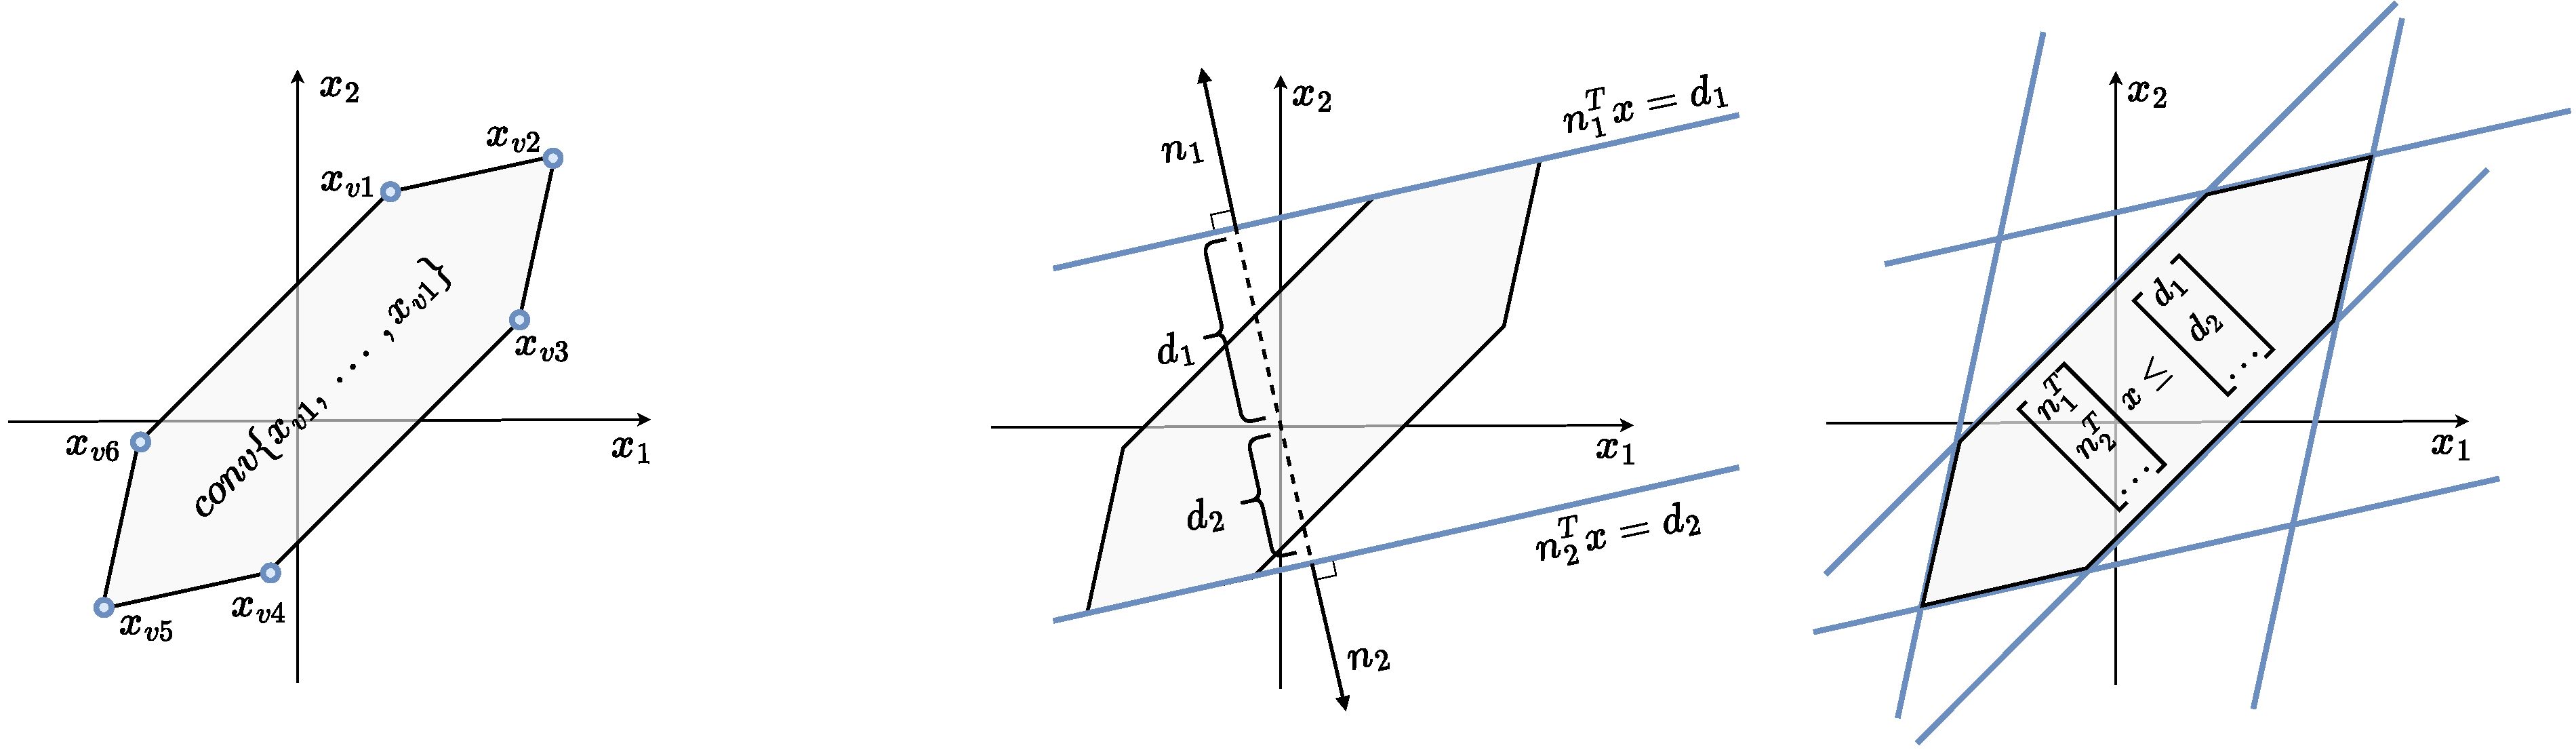
\includegraphics[width=\linewidth]{Chapters/imgs/h_v_rep.pdf}
    \caption{Figure illustrating the vertex ($\repr{V}$) and  half-plane ($\repr{H}$) representations of a polytope on a simple planar example. Image on the left shows the $\repr{V}$-representation as a Convex-Hull of the specified vertices. Images on the right show the $\repr{H}$-representation as an intersection of the half-planes (lines in 2D) representing the faces of the polytope $\mathcal{P}_x$.}
    \label{fig:hv_rep}
\end{figure}

Several alternative polytope representations were proposed recently, such as the $\repr{Z}$-representation \cite{kochdumper2019representation} where the polytopes are represented as polynomial zonotopes, and the $\repr{M}$-representation \cite{sigl2023mrepresentation} which is a more compact special case of the $\repr{Z}$-representation. These representations offer an improved efficiency of conducting polytope algebra operations, with respect to the traditional $\repr{H}$ and $\repr{V}$-representations. However, despite these advancements, their practical applications are still quite limited, primarily due to the challenging computational complexity involved in transforming polytopes into these alternative representations. 

Representing polytopes in these standard forms enables using different efficient tools from computational geometry and polytope algebra to perform operations over polytopes and provides tools for exploiting them in practical applications. However, in many cases polytope formulations do not correspond neither to the $\repr{V}$ nor $\repr{H}$-representation. As a result, many algorithms are developed in the literature transforming different polytope formulations into one of the two standard forms. The algorithms transforming the polytopes to the $\repr{V}$-representation are often called \textit{vertex enumeration} algorithms and to the $\repr{H}$-representation of are called \textit{facet enumeration} algorithms \cite{bremner_fukuda_marzetta_1998}. The appropriate choice of suitable polytope transformation algorithm, and its complexity, depends on various factors such as the polytope formulation, the desired polytope representation ($\repr{V}$ or $\repr{H}$), and potentially the time constraints for algorithm execution (online or offline). 

Therefore, \Cref{ch:generic_view} brings a structured overview of different polytopes, especially the ones occurring when characterising different physical abilities of humans and robots, and classifies them with respect to their formulation. \Cref{ch:polytope_algorithms} then exploits this classification to provide an overview of their applicable polytope transformation strategies and briefly discusses their efficiency.

\section{Generic view on physical ability polytope formulations}
\label{ch:generic_view}

This section aims to present a generic perspective on different families of polytope formulations commonly found when characterising the physical abilities of humans and robots. These polytopes are categorised based on their formulation to facilitate the choice of applicable algorithms.

From a generic standpoint, physical abilities represented in the shape of polytopes $\mathcal{P}_x$ can be seen as feasible sets of output (task space) variables $\bm{x} \in \mathbb{R}^m$, produced by applying a linear transformation on the input (actuation space) variables $\bm{y} \in \mathbb{R}^n$, bounded within (actuator limits) $\bm{y}\in\mathcal{P}_y$. As described in the previous chapter (\Cref{ch:collab_metrics_overview}), the polytope formulations for characterising physical abilities can be expressed in a unified generic form 
\begin{equation}
    \mathcal{P}_x = \{\bm{x}\in\mathbb{R}^m ~|~ A\bm{x}=B\bm{y} + \bm{b}, ~ \bm{y}\in\mathcal{P}_y\}
    \label{eq:generic_polyt_view_revisit}
\end{equation}
where matrices $B\in\mathbb{R}^{k\times n}$ and $A\in\mathbb{R}^{k\times m}$ present the linear transformation of the $n$ dimensional input to $m$ dimensional output space, through the $k$ dimensional intermediate space, while $\bm{b}\in\mathbb{R}^k$ is a bias vector. Furthermore, in the context of this work, the dimension of output space $m$ is considered to be lower or equal to the intermediate space dimension $k\!\geq\! m$ , which is in term lower or equal to the input space dimension $n\!\geq\! k\!\geq\! m$. In practice, this condition implies that the human or the robot model considered have at least the same number of degrees of freedom (DOF) as the dimension of the output space $m$. 

This compact and implicit formulation represents a unified view of different physical ability polytope formulations. However, depending on the structure of the matrices $A$ and $B$, as well as on the form of the input set $\mathcal{P}_y$, different algorithms are required to transform this formulation to its standard representations ($\repr{H}$ and $\repr{V}$). 

One important factor for determining the complexity of the polytope transformation, and the choice of the suitable algorithm, is the shape of the input set, corresponding to the limits of the input variable $\bm{y}\in\mathbb{R}^n$ limits. There are two most common forms that can be considered: interval form $\mathcal{I}_y$ and polytope form $\mathcal{P}_y$. 

The interval shaped $\mathcal{I}_y$ input set is specified in a form of min-max intervals
\begin{equation}
    \mathcal{I}_y = \{\bm{y}\in \mathbb{R}^n |~~ \bm{y}_{min} \leq \bm{y}\leq \bm{y}_{max} \}
    \label{eq:hypercube_lim}
\end{equation}
In a geometric sense, these individual intervals of the input variable $\bm{y}$ can be visualised as an $n$-dimensional hyperrectangle, also known as a hyperbox or an orthotope. Each axis $i$ of the hyperrectangle corresponds to an interval $y_i\in[y_{i,\text{min}},y_{i,\text{max}}]$.

More generally, rather than an interval $\mathcal{I}_y$, the input set can be defined as any convex polytope (ex. set of linear constraints in its $\repr{H}$-representation).
\begin{equation}
    \mathcal{P}_y = \{\bm{y}\in \mathbb{R}^n|~~ H_y\bm{y}\leq \bm{d}_y \}
\end{equation}

As polytopes $\mathcal{P}_x$ are then defined as linear transformations $A\bm{x}\!=\!B\bm{y}\! +\! \bm{b}$ of the input set (intervals $\mathcal{I}_y$ or polytope $\mathcal{P}_y$ shaped) from the input space to the output space, the structure of the linear transformation (matrices $A$ and $B$) has a direct impact on the complexity of the formulation, as well as on the choice of the algorithm.
Therefore, in this work, the distinction between two generic families of polytope formulations is proposed, derived from the unified formulation (\ref{eq:generic_polyt_view_revisit}): the projection formulation, where matrix $A$ is identity matrix $A=I_{m\times m}$, and the intersection formulation, where 
$B=I_{n\times n}$.

\subsection{Projection formulation}
\label{ch:proj_formulaiton}

\begin{figure}[!h]
    \centering
    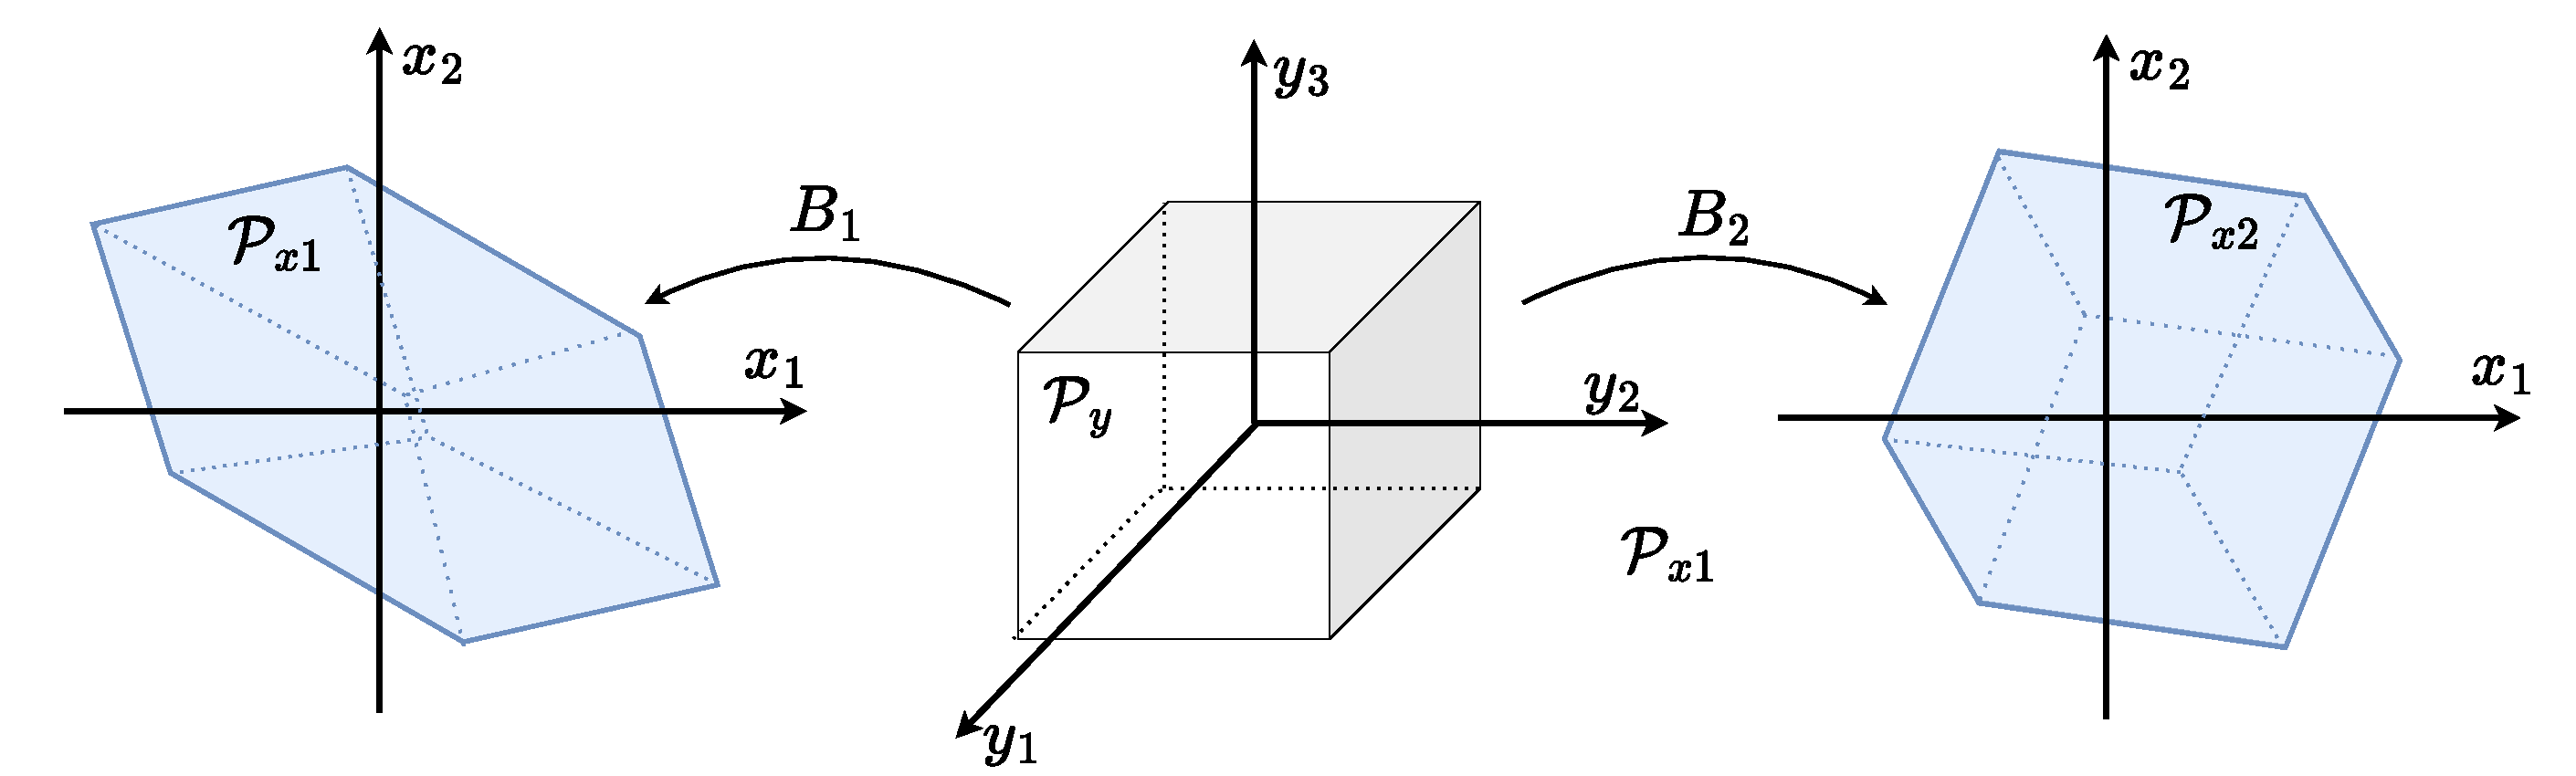
\includegraphics[width=0.8\linewidth]{Chapters/imgs/projection_double.pdf}
    \caption{An example ($m=2$, $n=3$) of constructing two different projection formulation polytopes, from the same input set $\mathcal{P}_y$. Polytopes $\mathcal{P}_{x1}$ and $\mathcal{P}_{x2}$ represent linear affine transformations of the input set $\mathcal{P}_y$ using two different transformation matrices $B_1$ and $B_2$.}
    \label{fig:proj_zono}
\end{figure}

The projection formulation is defined through a linear affine transformation of the $n$ dimensional input space $\bm{y}\in\mathbb{R}^n$ to the $m$ dimensional output space $\bm{x}\in\mathbb{R}^m$ using the projection matrix $B\in \mathbb{R}^{m\times n}$
\begin{equation}
    \mathcal{P}_x=\{\bm{x}\in \mathbb{R}^m ~|~ \bm{x} = B\bm{y} + \bm{b}_x,~\bm{y} \in\mathcal{P}_y \}
    \label{eq:proj_poly}
\end{equation}
where $\bm{b}_x\in\mathbb{R}^m$ is a constant bias vector, defined in the output space. The name \textit{projection} formulation comes from the fact that the polytope $\mathcal{P}_x$, in this formulation, is a projection of the $n$ dimensional input set $\mathcal{P}_y$ to the $m$ dimensional output space $\mathbb{R}^m$ \cite{Burger1996projection}.

A graphical representation of the projection formulation (\ref{eq:proj_poly}) is shown on \Cref{fig:image_projection_two}, where two different output polytopes $\mathcal{P}_x$ are constructed applying different affine transformation matrices $B$ on the same input set $\mathcal{P}_y$.


\subsubsection*{Zonotope formulation} If the input space has the interval shape $\mathcal{I}_y$, the final polytope $\mathcal{P}_x$, defined by the equation (\ref{eq:proj_poly}), has a zonotope form. In that case the polytope $\mathcal{P}_x$ can be represented as a Minkowski sum of $n$ line segments $\mathcal{L}_i$, each one corresponding to one axis range $[y_{i,min}, y_{i,max}]$ of the input set $\mathcal{I}_y$ projected to the output space using the matrix $B$.  \cite{McMullen1971onzonotopes}
\begin{equation}
    \mathcal{P}_x = \mathcal{L}_1 \oplus~ \cdots ~\oplus \mathcal{L}_n
\end{equation}
where the $i$-th line segment $\mathcal{L}_i$ can be expressed through $i$-th line vector $\bm{b}_i$ of the matrix $B$
\begin{equation}
    \mathcal{L}_i = \{\bm{x}\in\mathbb{R}^m ~|~ \bm{x} = \bm{b}_iy_i + \bm{b}_x,~~ y_i\in [y_{i,min}, y_{i,max}] \}
\end{equation}
\begin{wrapfigure}{r}{0.5\linewidth}
\vspace{-0.5cm}
% \begin{framed}
    \centering
    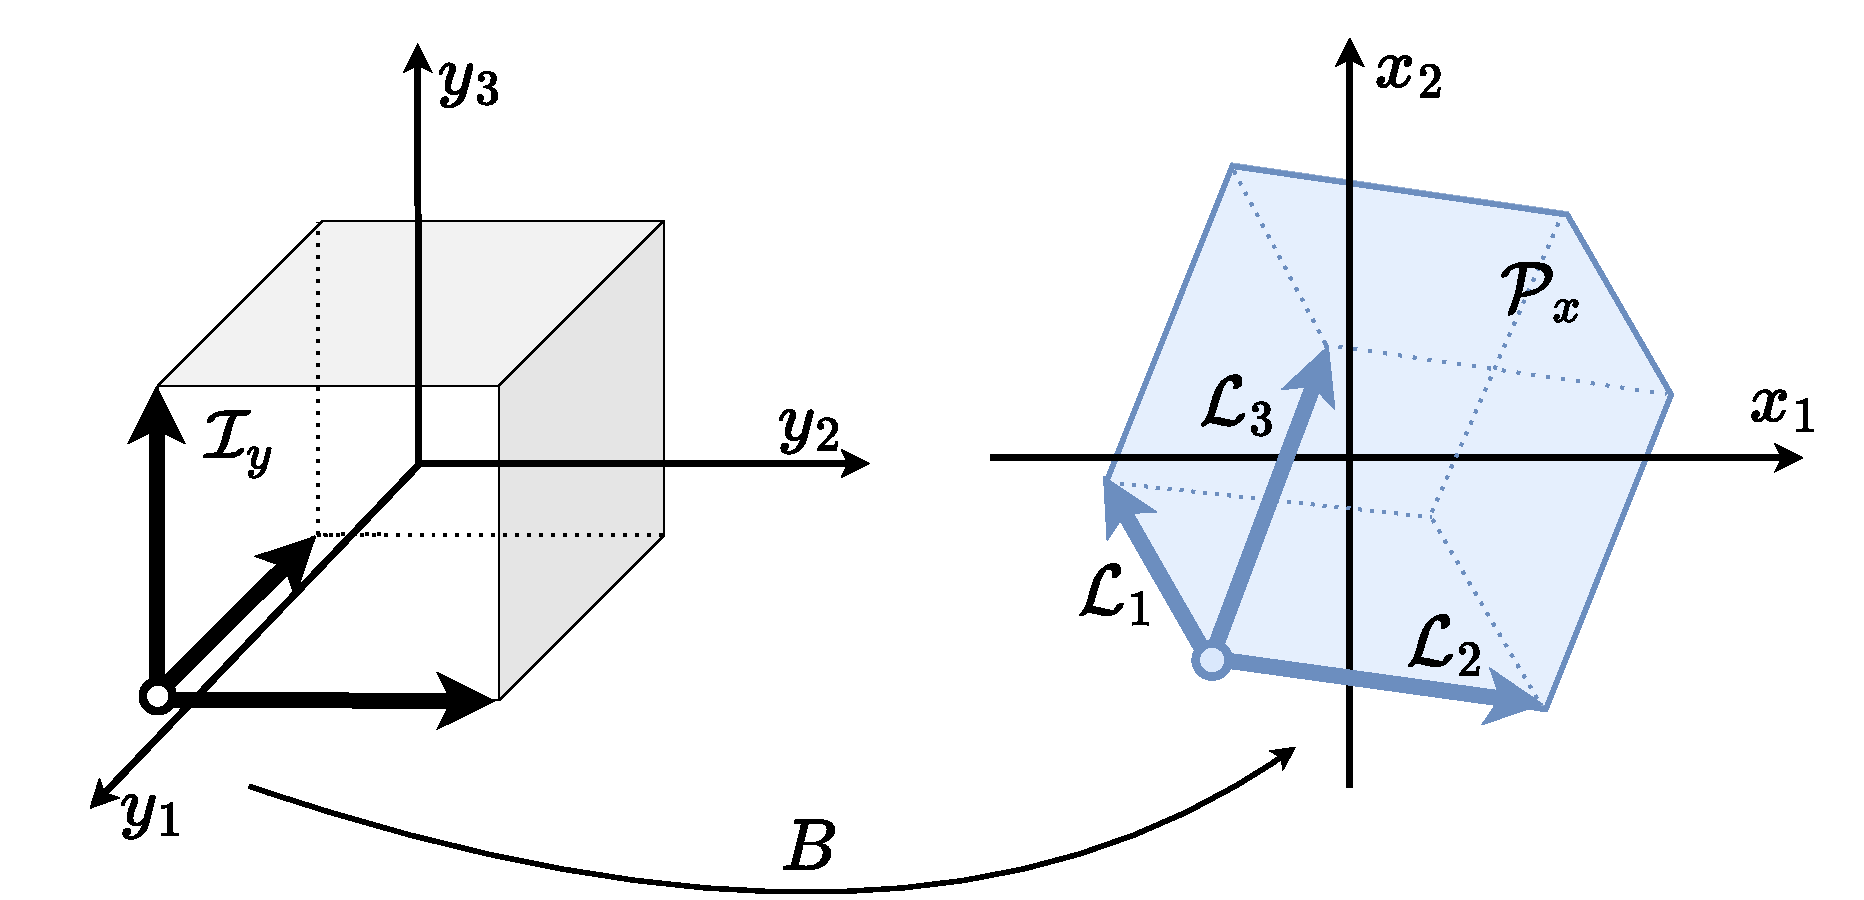
\includegraphics[width=\linewidth]{Chapters/imgs/zonotope_only.pdf}
    \caption{A graphical example ($m=2$, $n=3$) of constructing the zonotope shaped polytope $\mathcal{P}_x$ from the interval input set $\mathcal{I}_y$.}
    \label{fig:image_projection_two}
% \end{framed}
\end{wrapfigure}
These line segments are often called \textit{components} or \textit{generators} of the zonotope $\mathcal{P}_x$ \cite{shephard1974zonotopes}.

More generally, for any zonotope shaped input set $\mathcal{P}_y$, expressed as a Minkowski sum of the generators $\mathcal{L}_{yi}$
\begin{equation}
    \mathcal{P}_y = \mathcal{L}_{y1}  ~\oplus \mathcal{L}_{y2}~\oplus~ \cdots
\end{equation}
polytope $\mathcal{P}_x$ is a zonotope as well. The generators $\mathcal{L}_i$ of the polytope $\mathcal{P}_x$ correspond to the generators $\mathcal{L}_{yi}$ of the input set $\mathcal{P}_y$, projected to the output space using the equation (\ref{eq:proj_poly}). Therefore, polytope $\mathcal{P}_x$ has the same number of generators $\mathcal{L}_i$ as the zonotope $\mathcal{P}_y$, which can be expressed as
\begin{equation}
    \mathcal{L}_i = \{\bm{x}\in\mathbb{R}^m ~|~ \bm{x} = B\bm{y} + \bm{b}_x,~~ \bm{y}\in  \mathcal{L}_{yi}\}
\end{equation}

Zonotopes are highly structured and central symmetric shapes, hence transforming them to appropriate representations ($\repr{H}$ and $\repr{V}$) is in many cases more efficient than for generic polytopes.


\subsection{Intersection formulation}
\label{ch:inter_formulaiton}

\begin{figure}[!h]
    \centering
    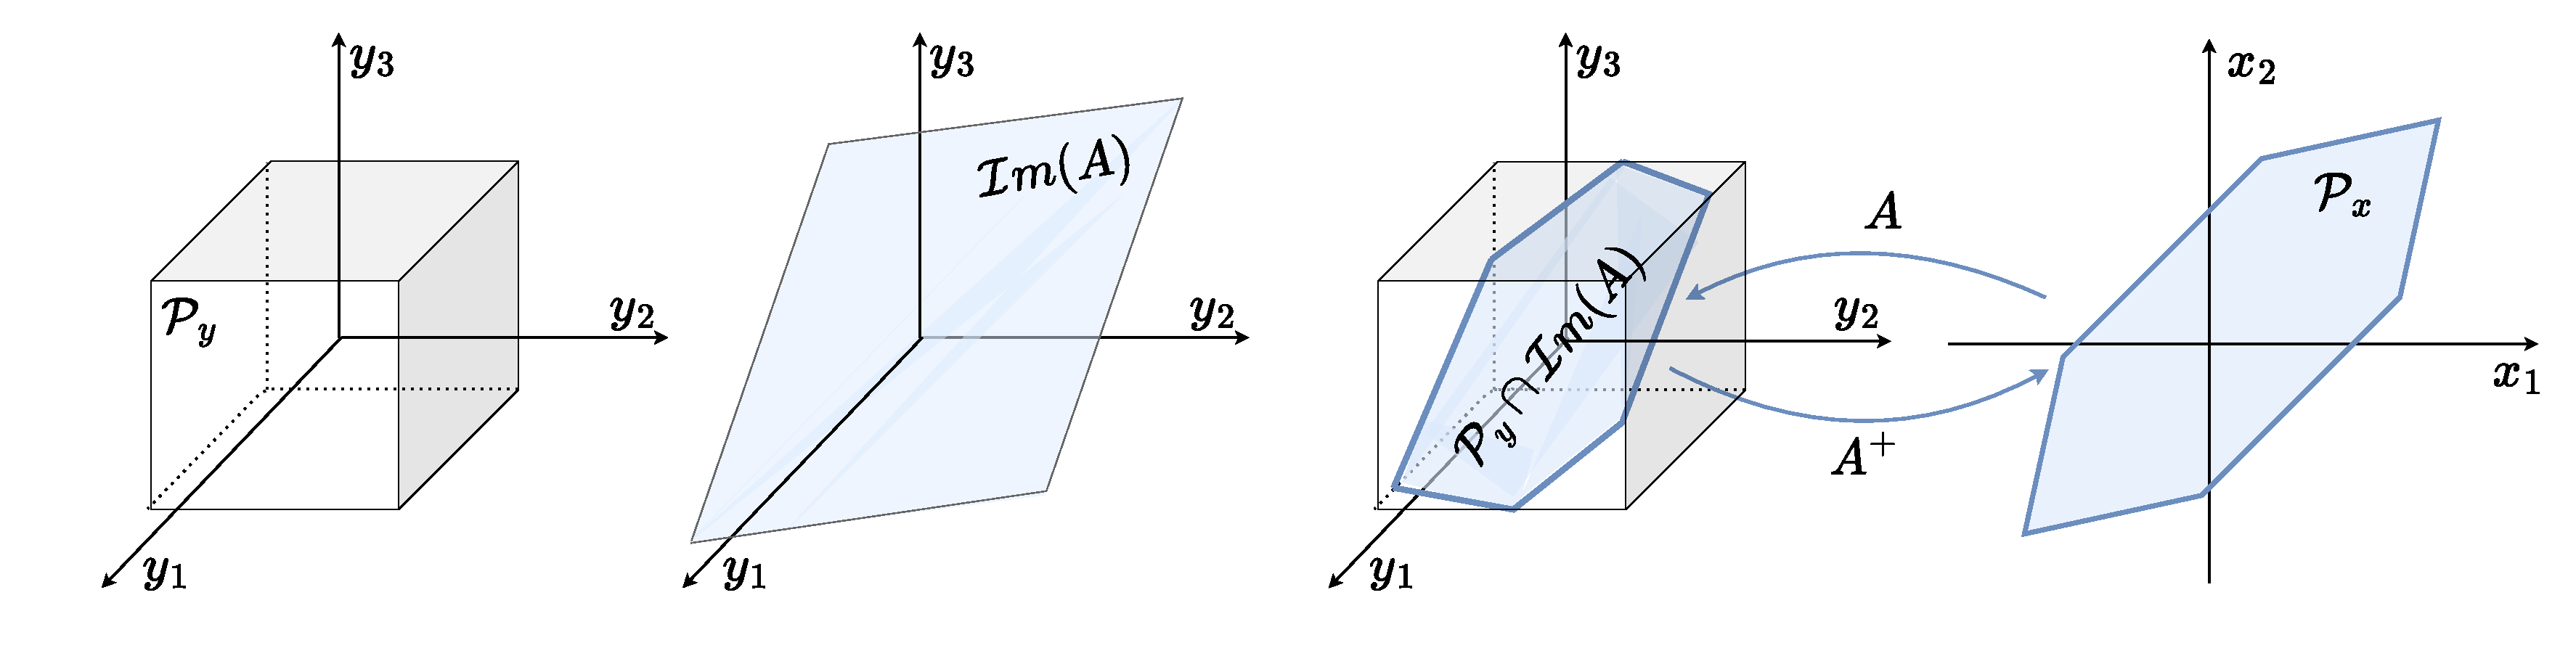
\includegraphics[width=\linewidth]{Chapters/imgs/image_intersection_poly_all.pdf}
    \caption{An example ($m=2$, $n=3$) of constructing a intersection formulation polytope $\mathcal{P}_x$ from the input set $\mathcal{P}_y$. First the image $\img{A}$ of the matrix $A$ is intersected with the input set $\mathcal{P}_y$, then this intersection is projected to the output space using the pseudo-inverse $A^+$. }
    \label{fig:inter_image_poly}
\end{figure}
The intersection formulation, on the other hand, is expressed by a matrix equation $A\bm{x}=\bm{y}$. It can be interpreted as a linear transformation in the opposite direction \cite{LARSON2013}, from the $m$ dimensional input space $\bm{x}\in\mathbb{R}^m$ to the $n$ dimensional output space $\bm{y}\in\mathbb{R}^n$, using the projection matrix $A\in \mathbb{R}^{n\times m }$
\begin{equation}
    \mathcal{P}_x=\{\bm{x} \in \mathbb{R}^m|~ A\bm{x} = \bm{y}+ \bm{b}_y,~ \bm{y} \in \mathcal{P}_y\}
    \label{eq:inter_poly}
\end{equation}
where $\bm{b}_y \in \mathbb{R}^n$ is a constant bias vector, defined in the input space. The name \textit{intersection} formulation comes from the fact that the polytope $\mathcal{P}_x$ is no longer just a projection of the input set $\mathcal{P}_y$ to the $m$ dimensional output space, but rather a projection of its intersection with the image $\img{A}$ of matrix $A$. 
A graphical representation of the intersection formulation (\ref{eq:inter_poly}) is shown on \Cref{fig:inter_image_poly}, where the intersection $\mathcal{P}_y\cap \img{A}$ and the final polytope $\mathcal{P}_x$ are denoted in blue.

The main difficulty of the intersection formulation (\ref{eq:inter_poly}) is that it is defined as an inverse projection, from the $m$ dimensional output space to the $n$ dimensional input space \cite{LARSON2013}. In order to inverse this relationship, an equivalent projection formulation polytope can be constructed by characterising the intersection $\mathcal{P}_y\cap \img{A}$. 

\subsubsection*{Equivalent projection formulation}\label{par:equivalent_proj} In order to express the intersection formulation in the projection form, it is necessary to inverse the relationship $\bm{y}=A\bm{x}$, considering $\bm{b}_y=\bm{0}$. If the input and output space have the same dimension $n=m$, $A$ is invertible and the inverse relationship can be easily obtained as $\bm{x} = A^{-1}\bm{y}$. 

\begin{wrapfigure}{r}{0.45\linewidth}
\vspace{-0.5cm}
% \begin{framed}
    \centering
    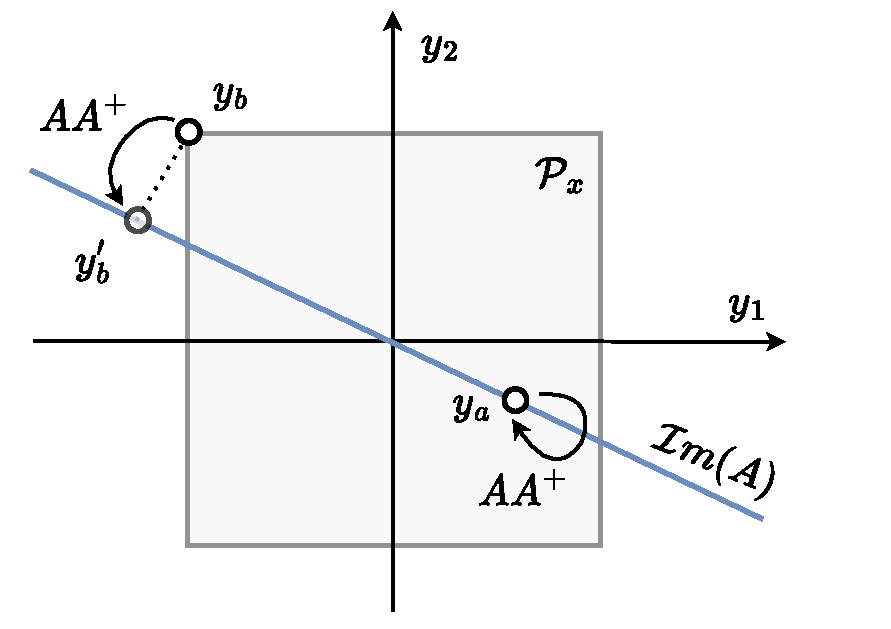
\includegraphics[width=\linewidth]{Chapters/imgs/img_pseudo_prob.pdf}
    \caption{An example ($n=2$,$m=1$) of applying the image projector $AA^+$ in the input space, the input set $\mathcal{P}_y$ is shown in grey and the image $\img{A}$ in blue. As the input vector $\bm{y}_a$ belongs to the image $\img{A}$ its multiplication with $AA^+$ results in the same vector. $\bm{y}_b$  does not belong to the image and $AA^+$ results in $\bm{y}_b'$, its orthogonal projection onto the image $\img{A}$ is outside the input set $\mathcal{P}_y$.}
    \label{fig:image_psueodinverse_ilustration}
% \end{framed}
\end{wrapfigure}

However, in the more general case, the input space is higher dimensional $n>m$, making  matrix $A$ not invertible. In such cases the inverse relationship can be obtained using the left pseudo-inverse of matrix $A$
\begin{equation}
    \bm{x} = (A^TA)^{-1}A^T\bm{y} = A^+\bm{y}
    \label{eq:pseudoinverse_equation}
\end{equation}

Due to the fact that, in the general case, the operation $\bm{x}\!=\!A^+\bm{y}$ is not bijective, the input vector $\bm{y}'\!=\!A\bm{x}$ corresponding to the output vector $\bm{x}\!=\!A^+\bm{y}$ does not correspond to the original input vector $\bm{y}$ 
\begin{equation}
\bm{y}' = A\bm{x} = A(A^+\bm{y})\neq\bm{y}
\end{equation}
making it possible that the input vector ${\bm{y}'\!=\!AA^+\bm{y}}$ no longer respects the input set $\mathcal{P}_y$
\begin{equation}
    \bm{y}'=AA^+\bm{y}\notin\mathcal{P}_y
\end{equation}

The matrix $AA^+$ represents an orthogonal projector matrix to the \textit{image space} $\img{A}$ of the matrix $A$ \cite[Chapter 5.5.4]{golub1996matrix}. Therefore, for any input vector $\bm{y}$ belonging to the image $\img{A}$, the multiplication by $AA^+$ results in itself \cite[Chapeter 1.3.1]{wang2018generalized}
\begin{equation}
    \bm{y} = AA^+\bm{y}, \qquad \forall \bm{y}\in\img{A}
    \label{eq:image_projector}
\end{equation}
However, for any input vector $\bm{y}$ not belonging to the image $\img{A}$, multiplying it with the matrix $AA^+$ will result in its orthogonal projection to the image $\img{A}$. As shown in the graphical example on \Cref{fig:image_psueodinverse_ilustration}, even though the original $\bm{y}$ respects the input set $\mathcal{P}_y$, its orthogonal projection onto the image $AA^+\bm{y}$ does not is some cases.

Therefore, having ensured that all the inputs $\bm{y}$ belong to the image $\img{A}$, the pseudo-inverse $A^+$ provides a unique inverse solution to the equation $\bm{y} = A\bm{x}$. Then, the new input set, respecting the limitations $\bm{y}\in\mathcal{P}_y$ and ensuring the unique inverse solution, can be found as the intersection
\begin{equation}
   \bm{y} \in \img{A} \cap \mathcal{P}_y
    \label{eq:intersection_ai}
\end{equation}
By exploiting the new input set and using the pseudo-inverse $A^+$, the equivalent formulation of the the initial intersection polytope $\mathcal{P}_x$ can be expressed as
\begin{equation}
\mathcal{P}_x=\{\bm{x}\in\mathbb{R}^m~|~ \bm{x} = A^+\bm{y} + A^+\bm{b}_y,~ \bm{y} \in \img{A}\cap\mathcal{P}_y\} \label{eq:proj_inter}
\end{equation}

Using the formulation (\ref{eq:proj_inter}), in practice, often requires characterising the image $\bm{y}\in\img{A}$ in a set form as well. As shown in expression (\ref{eq:image_projector}), all the vectors $\bm{y}$ belonging to the image $\img{A}$, when multiplied with the image projector $AA^+$ result in themselves ($\bm{y} - AA^+\bm{y} = \bm{0}$). This relationship can be exploited to formulate a compact set form of the image $\img{A}$ 
\begin{equation}
   \img{A} = \{ \bm{y}\in\mathbb{R}^n ~|~(I_{n\times n} - AA^+)\bm{y} = \bm{0}, \quad \bm{y}\in\mathbb{R}^n \}
   \label{eq:image_poly}
\end{equation}

\Cref{fig:inter_image_poly} provides a graphical representation of the mapping (\ref{eq:proj_inter}), showing the intersection $\img{A}\cap\mathcal{P}_y$ and the final polytope $\mathcal{P}_x$, being its projection to the output space $\bm{x}\in \mathbb{R}^m$. 

The intersection formulation is generally more computationally complex to work with than the projection formulation, as it often requires characterising the intersection $\img{A}\cap\mathcal{P}_y$. The graphical comparison of the construction of both intersection and projection polytopes from the same input set is shown on \Cref{fig:inter_proj}.


\begin{figure}
    \centering
    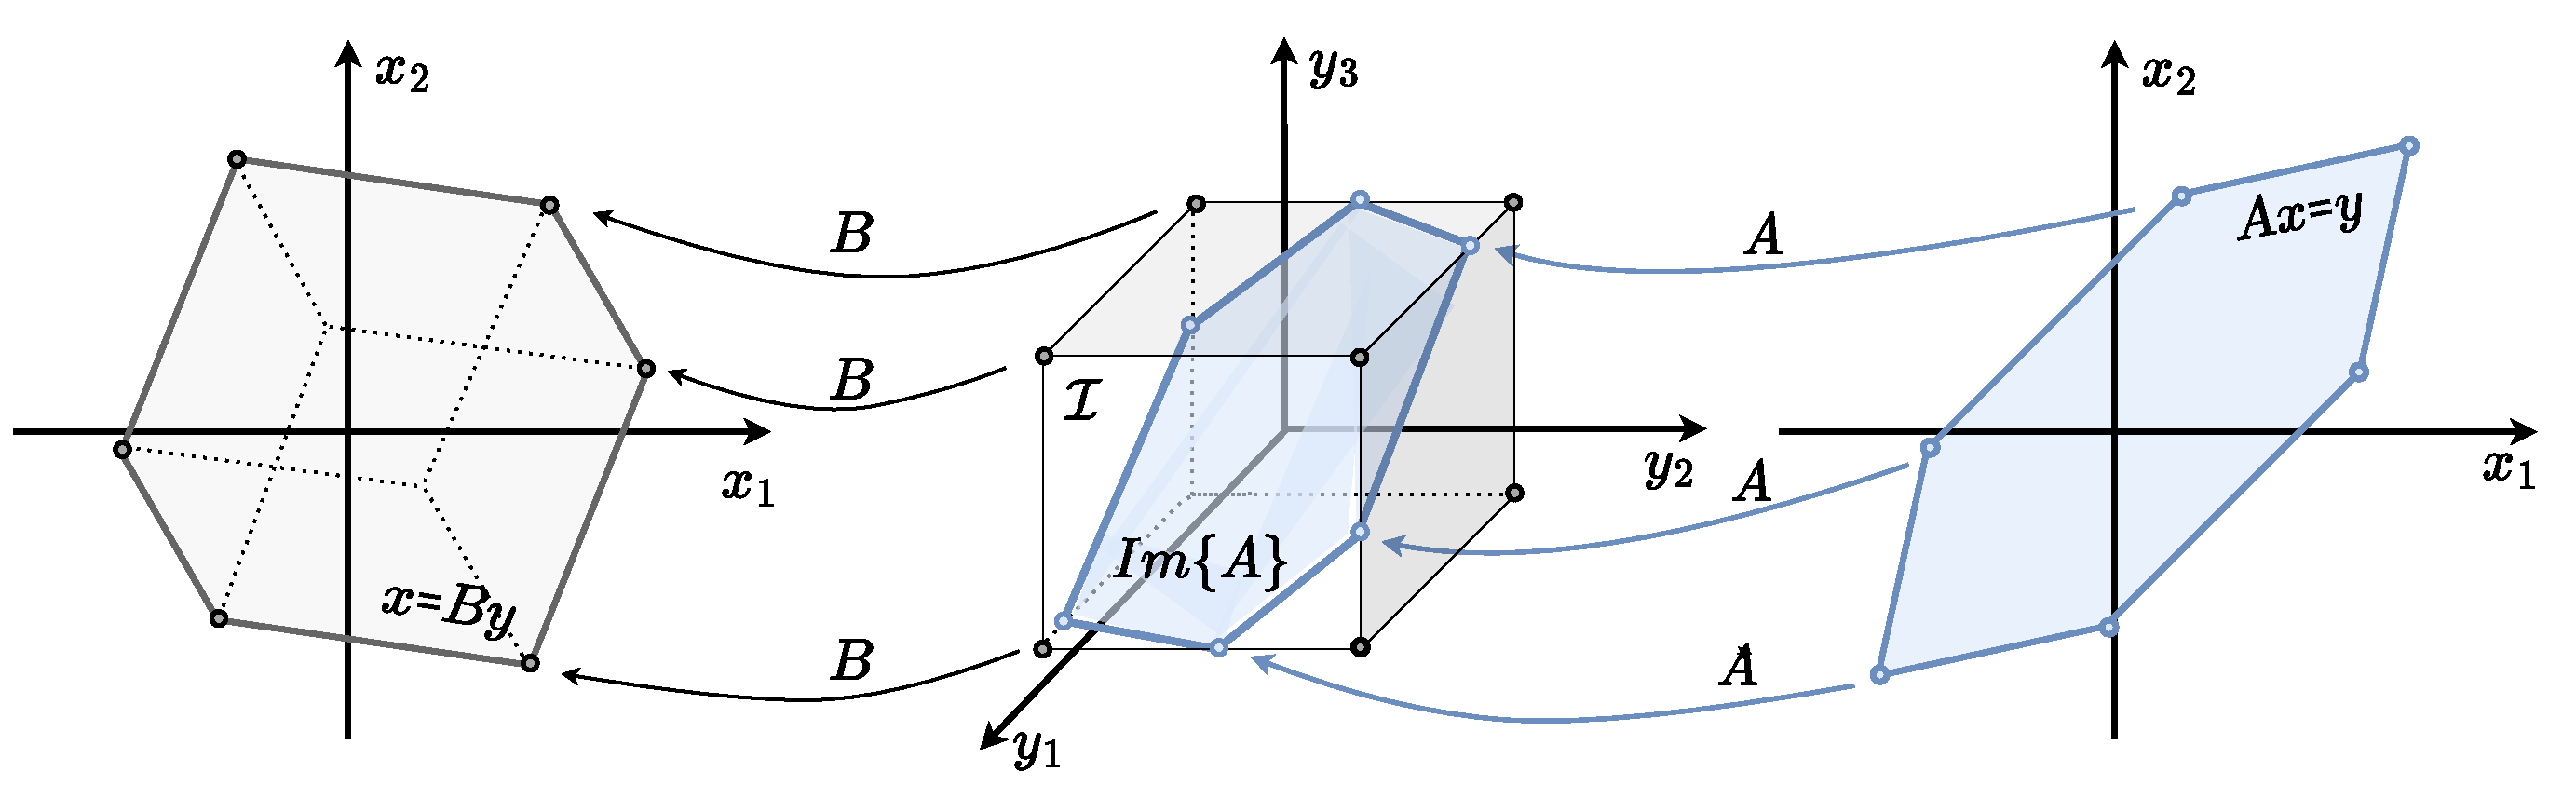
\includegraphics[width=\linewidth]{Chapters/imgs/intersection_projection.pdf}
    \caption{A comparative view of the projection (left) and intersection (right) polytope formulation using the same input space (middle). In the projection formulation, the whole input space $\mathcal{P}_y$ is projected using the matrix $B$ to the output space to obtain the polytope $\mathcal{P}_x$ (grey left). In the intersection formulation, first the intersection of the input space $\mathcal{P}_y$ with the image of the matrix $A$ is found (blue middle) $\img{A} \cap \mathcal{P}_y$, then this intersection can be projected to the output space using the pseudo-inverse $A^+$ of the matrix $A$ to obtain the polytope $\mathcal{P}_x$ (blue right).}
    \label{fig:inter_proj}
\end{figure}

\subsection{Combined cases}
\label{ch:combined_forms}
Physical ability polytopes described in \Cref{ch:human_metrics} contain two special cases consisting in the combination of intersection and projection polytope formulations: \textit{intersection-projection} and \textit{projection-intersection} formulation.

\subsubsection{Intersection-projection formulation}
\label{ch:inter_proj_form}

The unified generic polytope formulation given by the equation (\ref{eq:generic_polyt_view_revisit}) can be seen as a special case of the polytope formulation that contains both intersection and projection formulation
\begin{equation}
    \mathcal{P}_x \in \{\bm{x}\in \mathbb{R}^m~|~\underbrace{A \bm{x}= \bm{z}+ \bm{b}_z}_{\text{intersection}},~ \underbrace{ \bm{z}=B \bm{y}}_{\text{projection}} ,~ \bm{y} \in \mathcal{P}_y\} 
    \label{eq:inter_proj_poly}
\end{equation}
where $\bm{x}\in\mathbb{R}^m$ is the output vector, $\bm{y} \in \mathbb{R}^n$ is an input vector and $\bm{z}\in\mathbb{R}^k$ is an intermediate space vector, where $n\!\geq\!k\!\geq\!m$. Matrix $B\in \mathbb{R}^{k \times n}$ is a projector matrix from $n$ dimensional input space to the $k$ dimensional intermediate space, matrix $A\in \mathbb{R}^{k\times m}$ is a projector matrix from $m$ dimensional output space to the $k$ dimensional intermediate space and $\bm{b}_z\in\mathbb{R}^k$ is the bias vector, defined in the intermediate space.

In this work, this polytope formulation is named \textit{intersection-projection} as it is a special case of a intersection formulation (\ref{eq:inter_poly}) with polytope shaped input set which has the projection formulation. The final polytope $\mathcal{P}_x$ can be expressed as
\begin{equation}
    \mathcal{P}_x \in \{\bm{x}\in \mathbb{R}^m~|~A \bm{x} = \bm{z} + \bm{b}_z,~ \bm{z} \in \mathcal{P}_z\} 
\end{equation}
where its input set polytope $\mathcal{P}_z$ is defined using the projection formulation
\begin{equation}
    \mathcal{P}_z \in \{\bm{z}\in \mathbb{R}^k~|~z = B\bm{y},~ \bm{y} \in \mathcal{P}_y\} 
\end{equation}

\begin{figure}[!t]
    \centering
    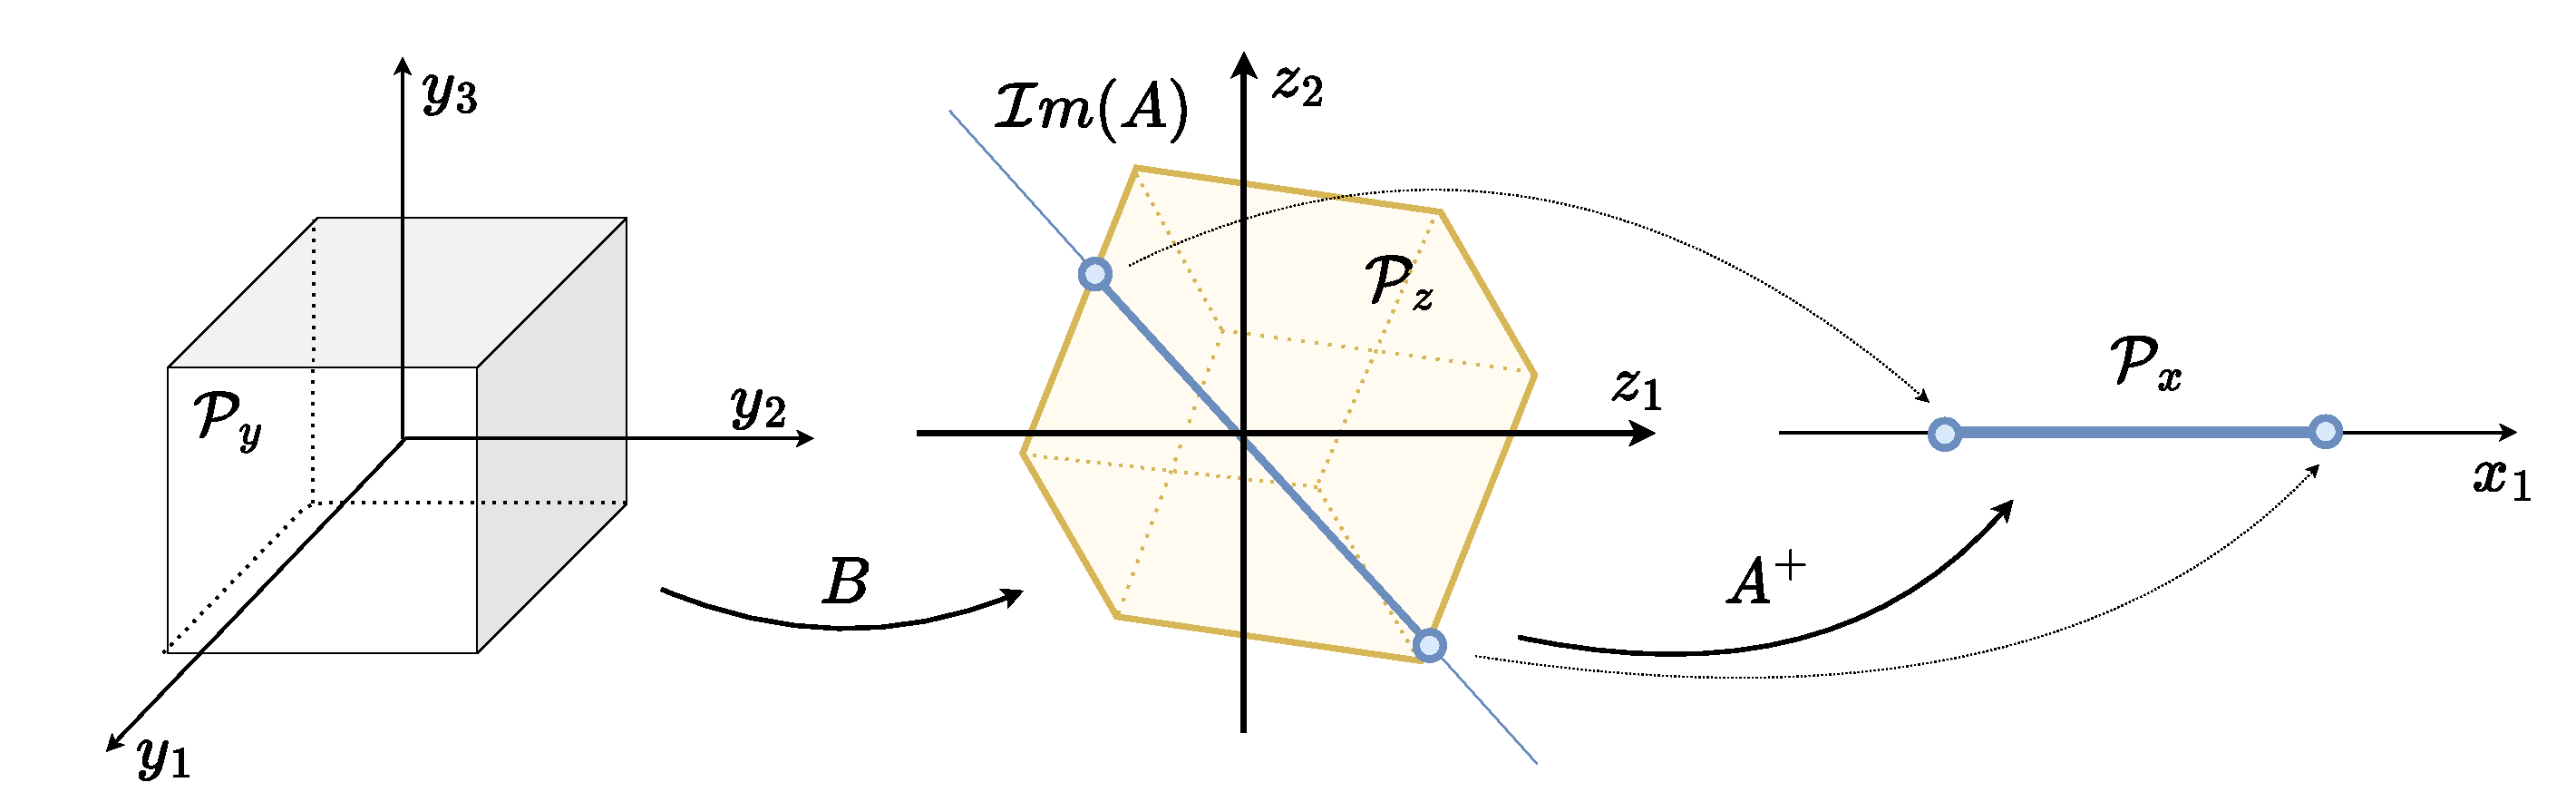
\includegraphics[width=\linewidth]{Chapters/imgs/spec_int_proj.pdf}
    \caption{An example ($n=3$, $k=2$, $m=1$) of a construction of the intersection-projection polytope $\mathcal{P}_x$ from the input set $\mathcal{P}_y$. Geometrically, first the input set $\mathcal{P}_y$ is projected to the intermediate space $\mathbb{R}^k$ to obtain the projection polytope $\mathcal{P}_z$ (yellow). Then this polytope is intersected with the image $\img{A}$ of matrix $A$ (blue middle). Finally the intersection $\mathcal{P}_z\cap\img{A}$ is projected to the output space with the pseudo-inverse $A^+$ to obtain the final 1D polytope $\mathcal{P}_x$ (blue right).}
    \label{fig:inter_proj_spec}
\end{figure}
This formulation can also be transformed to an equivalent projection formulation, as described for the intersection formulation is \Cref{par:equivalent_proj}, resulting in a polytope 
\begin{equation}
\mathcal{P}_x=\{\bm{x} \in \mathbb{R}^m |~ \bm{x} = A^+\bm{z} - A^+\bm{b}_z,~ \bm{z}+\bm{b}_z \in \img{A}\cap\mathcal{P}_z\} 
\end{equation}

However, this polytope formulation is much more computationally complex than both intersection and projection formulation, as it requires first computing the projection polytope $\mathcal{P}_z$ and then finding the intersection $\img{A}\cap\mathcal{P}_z$ in order to find the polytope $\mathcal{P}_x$. A graphical example of constructing the intersection-projection formulation polytope is shown on \Cref{fig:inter_proj_spec}.


\begin{remark}
    This formulation corresponds to the formulations of the wrench and stiffness capacity polytopes for human musculoskeletal models, described in \Cref{ch:force_poly_human} and \Cref{ch:human_stiffness_poly}.
\end{remark}


\subsubsection{Projection-intersection formulation}
\label{ch:proj_inter_form}

\begin{figure}
    \centering
    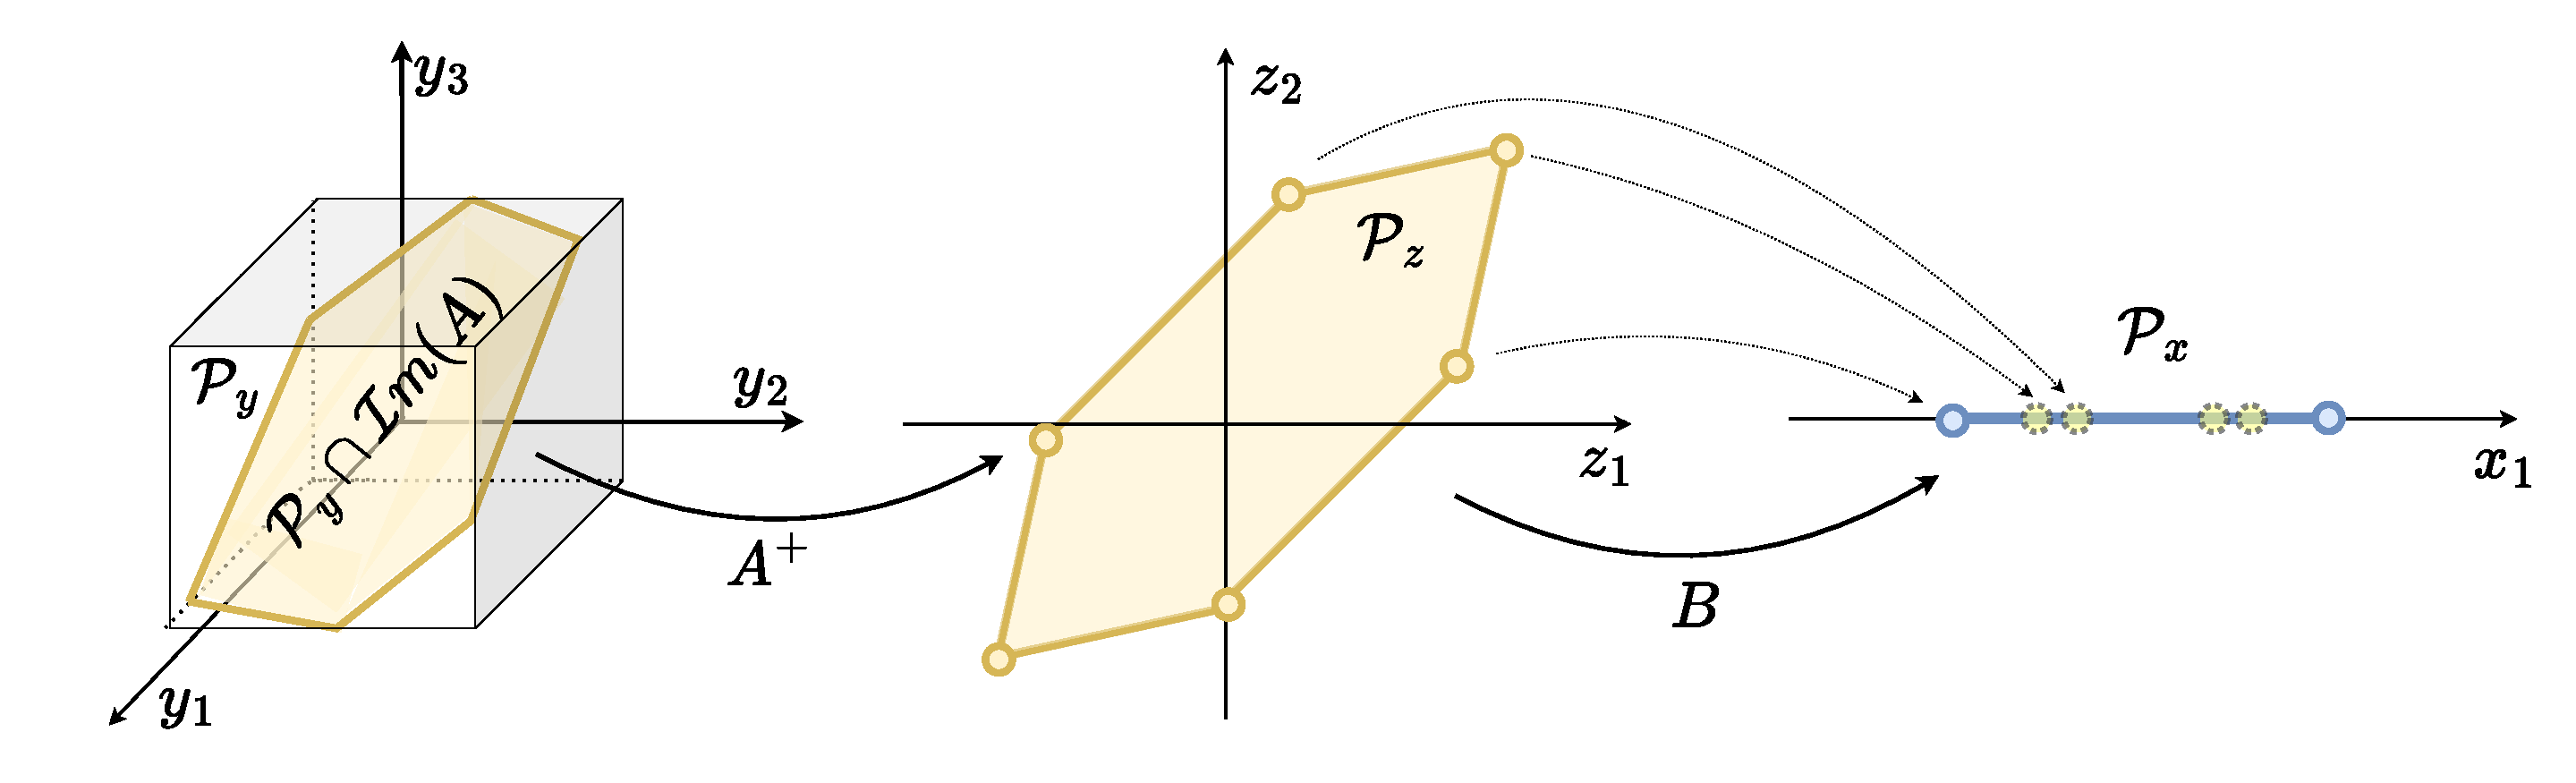
\includegraphics[width=\linewidth]{Chapters/imgs/spec_proj_int.pdf}
    \caption{An example ($n=3$, $k=2$, $m=1$) of a construction of the projection-intersection polytope $\mathcal{P}_x$ from the input set $\mathcal{P}_y$. 
    Geometrically, first the input set $\mathcal{P}_y$ is intersected with the image $\img{A}$ of the matrix $A$ (yellow left). The intersection $\mathcal{P}_y\cap\img{A}$ is then projected to the intermediate space using the pseudo-inverse $A^+$ to obtain the polytope $\mathcal{P}_z$ (yellow middle). Finally, an affine transformation $B$ is applied to the polytope $\mathcal{P}_z$ to transforming it to the final polytope 1D ($m=1$) $\mathcal{P}_x$ (blue right).}
    \label{fig:proj_inter_spec}
\end{figure}
A different special case of polytope formulation combining both projection and intersection formulation can be expressed as 
\begin{equation}
    \mathcal{P}_x \in \{\bm{x}\in \mathbb{R}^m~|~ \underbrace{\bm{x} = B \bm{z} + \bm{b}_x}_{\text{projection}},~ \underbrace{A\bm{z}=\bm{y}}_{\text{intersection}},~ \bm{y} \in \mathcal{P}_y\} 
    \label{eq:proj_inter_poly}
\end{equation}
where $\bm{x}\in\mathbb{R}^m$ is the output vector, $\bm{y} \in \mathbb{R}^n$ is an input vector and $\bm{z}\in\mathbb{R}^k$ is an intermediate space vector, where $n\!\geq\!k\!\geq\!m$. Matrix $A\in \mathbb{R}^{n\times k}$ is a projector matrix from $n$ dimensional input space to the $k$ dimensional intermediate space, matrix $B\in \mathbb{R}^{m\times k}$ is a projector matrix from $k$ dimensional intermediate space to the $m$ dimensional output space and $\bm{b}_x\in\mathbb{R}^m$ is the bias vector, defined in the output space.

In this work, this polytope formulation is named \textit{projection-intersection} as it is a special case of a projection formulation (\ref{eq:proj_poly}) with polytope shaped input set which has the intersection formulation. The final polytope $\mathcal{P}_x$ can be expressed as
\begin{equation}
    \mathcal{P}_x \in \{\bm{x}\in \mathbb{R}^m~|~ \bm{x} = B\bm{z} + \bm{b}_x,~ \bm{z} \in \mathcal{P}_z\} 
\end{equation}
where its input set polytope $\mathcal{P}_z$ is defined using the intersection formulation
\begin{equation}
    \mathcal{P}_z \in \{\bm{z}\in \mathbb{R}^n~|~Az = \bm{y},~ \bm{y} \in \mathcal{P}_y\} 
\end{equation}

This formulation can also be transformed to an equivalent projection formulation, using the same procedure described in \Cref{par:equivalent_proj}, resulting in a polytope 
\begin{equation}
\mathcal{P}_x=\{\bm{x} \in \mathbb{R}^m |~ \bm{x} = BA^+\bm{y} + \bm{b}_x,~ \bm{y}\in \img{A}\cap\mathcal{P}_y\} 
\end{equation}

This polytope formulation is again much more computationally complex than both intersection and projection formulation, as it requires first computing the intersection $\bm{y} \in \img{A}\cap\mathcal{P}_y$, followed by the projection $BA^{+}\bm{y}$. A graphical example of constructing the projection-intersection formulation polytope is shown on \Cref{fig:proj_inter_spec}.

\begin{remark}
    This generic formulation corresponds to the formulation of the velocity capacity polytope for human musculoskeletal models, described in the \Cref{ch:human_vel_poly}.
\end{remark}


\subsection{Synthesis of polytope formulations}
\label{ch:which_metric_which_formulation}

\Cref{ch:generic_view} proposes a structured view on different families of polytope formulations, with the aim to group the polytope formulations that can be used with the same polytope transformation algorithms. The discussed families are based on the generic polytope formulation (\ref{eq:generic_polyt_view_revisit}), 
\begin{equation}
    \mathcal{P}_x = \{\bm{x}\in\mathbb{R}^m ~|~ A\bm{x}=B\bm{y} + \bm{b}, ~ \bm{y}\in\mathcal{P}_y\}
    \label{eq:generic_polyt_view_revisit4}
\end{equation}
which, as described in \Cref{ch:phisical_ability_metrics} (synthesis \Cref{ch:collab_metrics_overview}), unifies all the common polytope representations for characterising physical abilities of robots and humans. 

There are two main families of polytope formulations discussed in this section: projection and intersection polytope formulation. 

The projection formulation (\ref{eq:proj_hyp}) corresponds to the specific case of the formulation  (\ref{eq:generic_polyt_view_revisit4}) where the matrix $A$ is an identity matrix $I_{m\times m}$.
The projection formulation is defined as the linear affine transformation of the input set $\mathcal{P}_y$ into the output space through the matrix $B$, forming the polytope $\mathcal{P}_x$. 

The intersection formulation (\ref{eq:inter_poly}) corresponds to the specific case of the formulation 
(\ref{eq:generic_polyt_view_revisit4}) where matrix $B$ is an identity matrix $I_{n\times n}$. As described in \Cref{ch:inter_formulaiton}, the polytopes $\mathcal{P}_x$ expressed in this formulation can be seen geometrically as a linear projection of the intersection of the input set $\mathcal{P}_y$ and the image space $\img{A}$ of the matrix $A$, to the output space. 

Furthermore, two special cases of these formulations are discussed in \Cref{ch:combined_forms} intersection-projection formulation, corresponding to the intersection polytope where the input set $\mathcal{P}_y$ has the projection formulation, and projection-intersection formulation, corresponding to the projection polytope where the input set $\mathcal{P}_y$ has the intersection formulation. 

\Cref{tab:generic_formulations} shows, in a condensed manner, how the introduced polytope forms correspond to the generic formulation (\ref{eq:generic_polyt_view_revisit4}).

% \begin{table}
% \centering
% \begin{tabular}{|l|c|c|}
% \hline
% Formulation & Equation & Formulation $\mathcal{P}_x$\\
% \hline
% Projection  & \ref{eq:proj_poly}& $\{\bm{x}\in\mathbb{R}^m~|~\bm{x}=B\bm{y} + \bm{b}_x, ~\bm{y}\in\mathcal{P}_y\}$\\
% Intersection  & \ref{eq:inter_poly}& $  \{\bm{x}\in\mathbb{R}^m~|~A\bm{x}=\bm{y} + \bm{b}_y, ~\bm{y}\in\mathcal{P}_y\}$\\
% \hline
%  \multicolumn{3}{c}{Special cases} \\
% \hline
% Intersection-Projection  & \ref{eq:inter_proj_poly}& $ \{\bm{x}\in\mathbb{R}^m~|~A\bm{x}=B\bm{y} + \bm{b}_z, ~\bm{y}\in\mathcal{P}_y\}$\\
% Projection-intersection & \ref{eq:proj_inter_poly}& $ \{\bm{x}\in\mathbb{R}^m~|~\bm{x}=B\bm{z} + \bm{b}_x, ~ A\bm{z}=\bm{y}, ~\bm{y}\in\mathcal{P}_y\}$\\
% \hline
% \end{tabular}
% \caption{Comparison of Polytope-based Physical Ability Metrics}
% \label{tab:formulation_input_comparison}
% \end{table}

\begin{table}[!h]
\centering
\begin{tabular}{|l|c|c|c|c|c|c|c|c|c|}
\hline
Formulation & Eqn. & $\bm{x}$ & $A$ & $B$ & $\bm{y}$ & Input set $\mathcal{P}_y$ & $\bm{b}$ \\
\hline
Projection & \ref{eq:proj_poly} & $\bm{x}\in\mathbb{R}^m$ & $I_{m\times m}$& $B$ & $\bm{y}\in\mathbb{R}^n$ & $\mathcal{P}_y$ & $\bm{b}_x\in\mathbb{R}^m$ \\
Intersection & \ref{eq:inter_poly} & $\bm{x}\in\mathbb{R}^m$ & $A$& $I_{n\times n}$ & $\bm{y}\in\mathbb{R}^n$ & $\mathcal{P}_y$ & $\bm{b}_y\in\mathbb{R}^n$ \\
\hline
\multicolumn{10}{c}{Combined cases} \\
\hline
Intersection-projection & \ref{eq:inter_proj_poly} & $\bm{x}\in\mathbb{R}^m$ & $A$& $B$ & $\bm{y}\in\mathbb{R}^n$ & $\mathcal{P}_y$ & $\bm{b}_z\in\mathbb{R}^k$ \\
Projection-intersection & \ref{eq:proj_inter_poly} & $\bm{x}\in\mathbb{R}^m$ & $I_{m\times m}$& $B$ & $\bm{z}\in\mathbb{R}^k$ & $\mathcal{P}_z$ & $\bm{b}_x\in\mathbb{R}^m$ \\
\hline
\end{tabular}
\caption{Ths table brings the correspondence in the introduced polytope formulations and the generic formulation (\ref{eq:generic_polyt_view_revisit4}). }
\label{tab:generic_formulations}
\end{table}

The following sections leverage the proposed view on different polytope formulations and provide an overview of standard algorithms for transforming these families of polytope formulations to standard polytope representations ($\repr{H}$ and $\repr{V}$). 

% \begin{table}
% \centering
% \begin{tabular}{|l|c|c|c|c|c|}
% \hline
% Polytope Metric & Equation & $\bm{x}$ & Formulation &  $\bm{y}$ & Input set $\mathcal{I}$ \\
% \hline
%  \multicolumn{6}{c}{Robotic manipulators} \\
% \hline
% Velocity  & \ref{eq:poly_vel_rob}& $\dot{\bm{x}}$ & projection & $\dot{\bm{q}}$&$\dot{\bm{q}} \in [\dot{\bm{q}}_{min},\dot{\bm{q}}_{max}]$ \\
% Kinematic Acceleration  & \ref{eq:poly_accel_kin} & $\ddot{\bm{x}}$  & projection & $\ddot{\bm{q}}$&$\ddot{\bm{q}}\in\ddot{\bm{q}}_{min},\ddot{\bm{q}}_{max}]$   \\
% Kinematic Jerk  &\ref{eq:poly_jerk_kin} & $\dddot{\bm{x}}$ &  projection &$\dddot{\bm{q}}$&$\dddot{\bm{q}}\in[\dddot{\bm{q}}_{min},\dddot{\bm{q}}_{max}]$ \\
% Precision  & \ref{eq:poly_precision_rob} & $\delta\dot{\bm{x}}$ & projection & $\delta{\bm{q}}$&$\delta{\bm{q}}\in[\delta{\bm{q}}_{min},\delta{\bm{q}}_{max}]$ \\
% Force/Wrench &  \ref{eq:poly_force_rob} & $\bm{f}$ & intersection & $\bm{\tau}$&$\bm{\tau}\in [\bm{\tau}_{min},\bm{\tau}_{max}]$ \\
% Acceleration  & \ref{eq:pol_accleration_rob} & $\ddot{\bm{x}}$ & projection & $\bm{\tau}$&$\bm{\tau}\in[\bm{\tau}_{min},\bm{\tau}_{max}]$ \\
% Stiffness feasibility  &  \ref{eq:pol_sfr_rob}& $\Delta\bm{x}$ & intersection &$\bm{\tau}$&$\bm{\tau}\in[\bm{\tau}_{min},\bm{\tau}_{max}]$\\
% \hline
%  \multicolumn{6}{c}{Human musculoskeletal models} \\
% \hline
% Velocity &\ref{eq:velocity_polytope_human_ver_poly_lim}  & $\dot{\bm{x}}$ & projection & $\dot{\bm{q}}$&$\dot{\bm{q}}\in\mathcal{P}_{\dot{\bm{q}}}$ \\
% % Force/Wrench & $\bm{f}$ & $J^T$ & $N$ & $[\bm{F}_{min},\bm{F}_{max}]$ & $\bm{F}$ & $\bm{\tau}_b$ \\
% Force/Wrench & \ref{eq:human_force_poly_ver_poly_lim} &  $\bm{f}$ & intersection & $\bm{\tau}$&$\bm{\tau}\in\mathcal{P}_{\bm{\tau}}$ \\
% Acceleration  & \ref{eq:poly_acceleration_hum} & $\ddot{\bm{x}}$ &projection & $\bm{F}$&$\bm{F}\in[\bm{F}_{min},\bm{F}_{max}]$  \\
% % Stiffness feasibility  &$\Delta\bm{x}$ & $J^T$ & $N$ & $[\bm{F}_{min},\bm{F}_{max}]$ & $\bm{F}$ & $\bm{\tau}_b$ \\
% Stiffness feasibility & \ref{eq:stiffness_human_all}  &$\Delta\bm{x}$  & intersection & $\bm{\tau}$&$\bm{\tau}\in\mathcal{P}_{\bm{\tau}}$ \\
% \hline
% \end{tabular}
% \caption{Comparison of Polytope-based Physical Ability Metrics}
% \label{tab:formulation_input_comparison}
% \end{table}


\section{An overview of polytope transformation strategies} 
\label{ch:polytope_algorithms}

Transforming polytopes to their standard representations ($\repr{V}$ and $\repr{H}$) is a well studied problem in literature. Over the years, many efficient algorithms  \cite{bremner_fukuda_marzetta_1998,fukuda_dd,avis_pivoting_nodate} have been proposed for vertex enumeration, finding the $\repr{V}$-representation, and facet enumeration, finding the $\repr{H}$-representation. 

However, the algorithms are often developed for a specific polytope formulation, where their efficiency might vary considerably with the size of the problem (dimension of input and output spaces) \cite{avis_comparative_2015} and the complexity of the evaluated polytope (number of faces and vertices) \cite{Dyer1983}. Therefore, the choice of the appropriate polytope transformation algorithm depends on to the polytope formulation, the representation required by the application, as well as the required time-efficiency.

This section brings a non-exhaustive overview of standard algorithms for transforming different polytope formulations (intersection and projection) with different input set shapes (interval $\mathcal{I}_y$ and polytope $\mathcal{P}_y$) into different standard representations ($\repr{V}$ and $\repr{H}$). Additionally, \Cref{ch:approximation_algos} discusses different polytope approximation strategies in the context of improving the efficiency of the vertex and half-plane evaluation. Finally, \Cref{ch:overview_algo_synthesis} brings a condensed view of the proposed overview in a form of \Cref{tab:algorithms table}.

\subsection{Standard polytope representation conversion algorithms}
\label{ch:standard_represtantion_conversion}

Converting polytope representations from half-plane ($\repr{H}$) to vertex ($\repr{V}$) and \textit{vice-versa} is a well studied problem in literature. Many different algorithms have been developed capable of performing the transformations in both directions, with various degrees of efficiency. 

There are two main families of approaches developed in the literature: \gls{ina} and \gls{gta} \cite[Chapter 8.]{fukuda2016lecture} \cite{avis1997how}.

\glsxtrfull{ina} construct the $\repr{V}$-representation of polytopes by iteratively intersecting the half-planes defined by the $\repr{H}$-representation, while keeping only the intersection points that correspond to the vertices of the polytope. These methods construct the $\repr{H}$-representation in an iterative manner as well, by constructing the half-plane equations from the vertices and keeping only the ones corresponding to the faces of the polytope. Examples of incremental algorithms are the \gls{ddm} \cite{MotzkinR1953dd,fukuda_dd} or the Beneath and beyond method \cite{Seidel_1981}.

\glsxtrfull{gta} are based on representing the polytope in a form of a graph of its vertices connected by its edges. This graph is then traversed in different fashions in order to obtain all the vertices ($\repr{V}$-representation) and faces ($\repr{H}$-representation) of the polytope. Examples of such methods are the \gls{pim} by \citet{bremner_fukuda_marzetta_1998}, the Gift-wrapping algorithm by Seidel \cite{Seidel1987outputsensitive} of the Reverse search algorithm by Avis and Fukuda \cite{avis_pivoting_nodate}

A comprehensive review of different conversion algorithm was proposed by \citet{avis1997how}, comparing the efficiency of different families of algorithms on different standard polytope benchmarks, as well as their available implementations. In general, the \gls{gta} methods are more efficient for higher dimensional problems, while \gls{ina} methods are more efficient for lower dimensional problems, for dimensions up to 12 \cite[Chapter 8.3]{fukuda2016lecture}.

These methods are standard building blocks for using polytopes in practical applications as well as for computing different operations over polytopes, such as intersections, Convex-Hulls and Minkowski sums (described in \Cref{ch:operations_over_poly_stategies}). However, the polytope formulations families described in the previous section are not expressed neither as $\repr{H}$ nor $\repr{V}$-representation. Therefore, these formulations require either additional steps in order to be used with standard \gls{ina} or \gls{gta} algorithms, or in some cases, dedicated algorithms that are specific to their formulations. 


\subsection{Strategies for the intersection formulation}
\label{ch:intersection_algos}

This section brings an overview of approaches used for transformation of polytopes with the intersection formulation, described in \Cref{ch:inter_formulaiton}, into their respective $\repr{V}$ and $\repr{H}$-representation. 

The polytopes with the intersection formulation can be expressed as
\begin{equation}
    \mathcal{P}_x=\{\bm{x}\in\mathbb{R}^m |~ A\bm{x} = \bm{y} + \bm{b}_y,~\bm{y} \in \mathcal{P}_y  \}
    \label{eq:inter_poly_revist}
\end{equation}
where $\bm{y}\in\mathbb{R}^n$, $\bm{b}_y\in\mathbb{R}^n$ are the $n$ dimensional input vector and input bias, $\bm{x}\in\mathbb{R}^m$ is the $m$ dimensional output vector, $A\in\mathbb{R}^{n\times n}$ is a transformation matrix from output to the input space and $\mathcal{P}_y$ is the input set.

\label{ch:inter_poly_chapter}
\begin{figure}[!t]
    \centering
    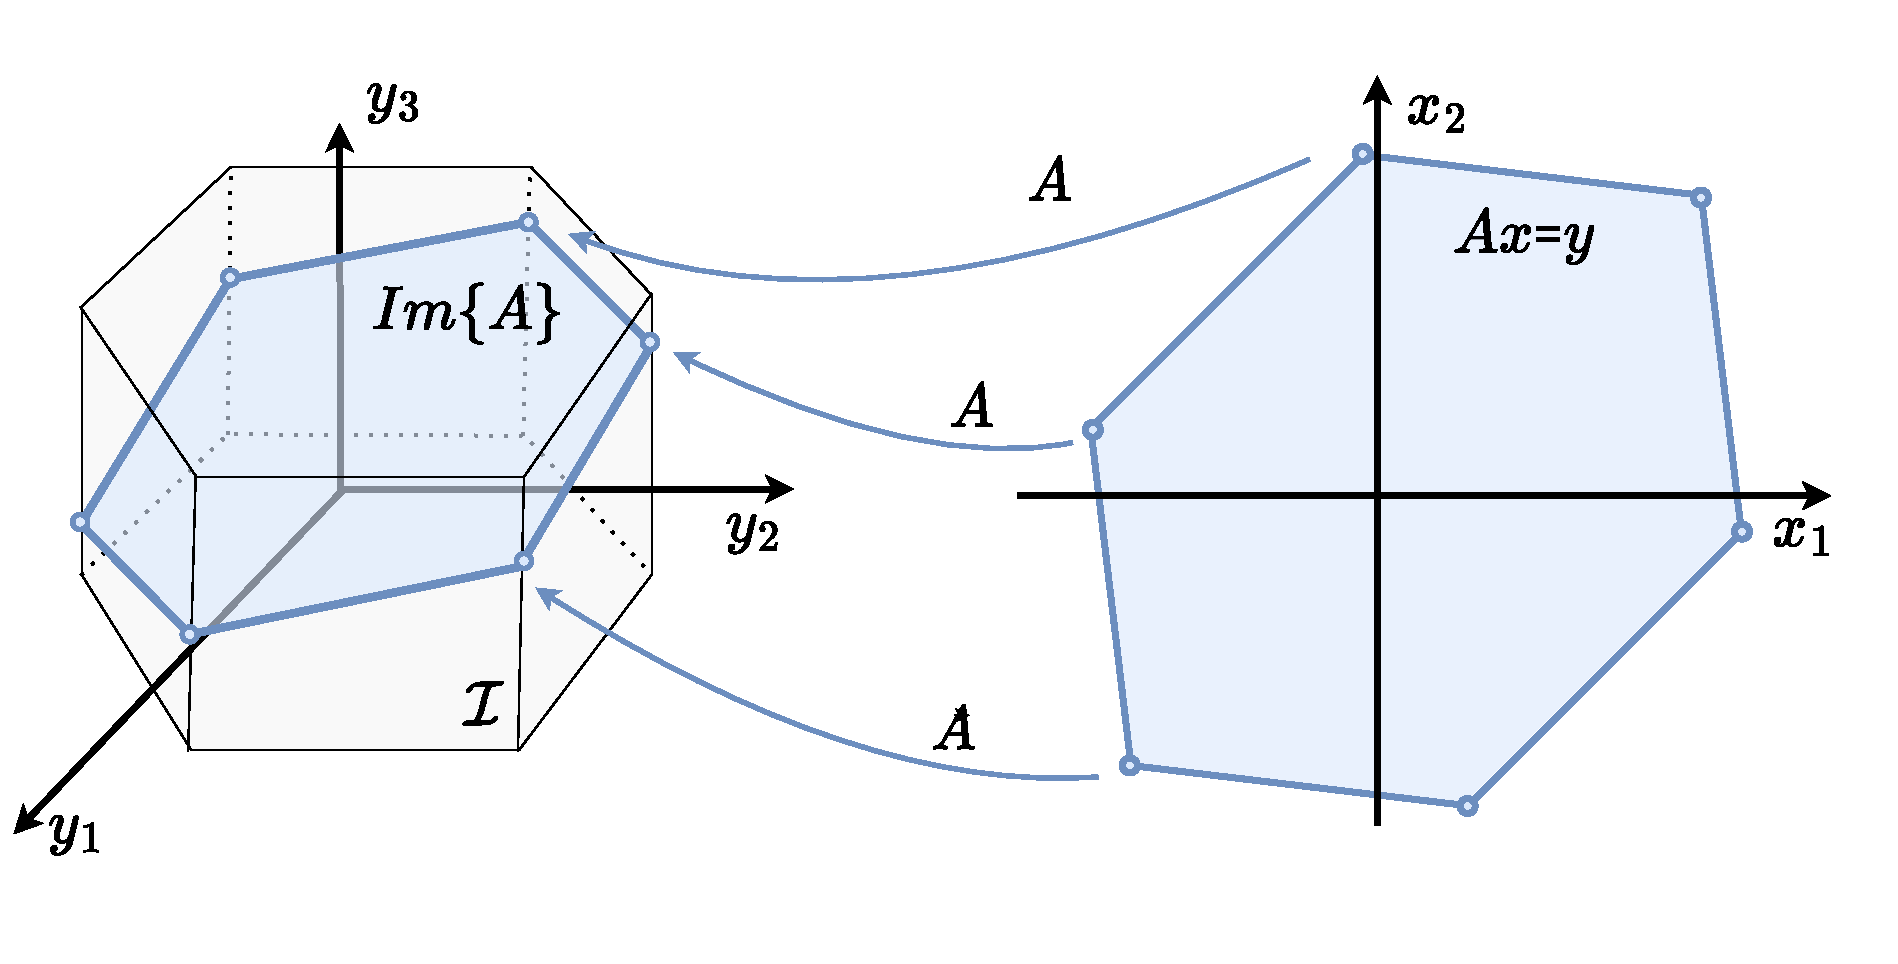
\includegraphics[width=0.8\linewidth]{Chapters/imgs/inter_poly.pdf}
    \caption{An example of constructing an intersection formulation polytope with an $m=2$ dimensional output space and an $n=3$ dimensional input space. The input set $\mathcal{P}_y$ has a polytope form, and its intersection with the image of the matrix $A$ is shown in blue (left). The final polytope $\mathcal{P}_x$ is shown in blue as well (right).}
    \label{fig:inter_poly}
\end{figure}

The geometrical representation of the polytope $\mathcal{P}_x$ defined by (\ref{eq:inter_poly_revist}) is shown on \Cref{fig:inter_poly}, for the example of $n=3$ dimensional input set $\mathcal{P}_y$ and $m=2$ dimensional polytope $\mathcal{P}_x$. 
The resulting polytope $\mathcal{P}_x$ is an affine projection of the intersection of the input polytope $\mathcal{P}_y$ and the image $\img{A}$ of the matrix $A$ into the lower dimensional output space. As shown on \Cref{fig:inter_poly}, the vertices and faces of the polytope $\mathcal{P}_x$ do not correspond to the projection of the vertices and faces of the input polytope $\mathcal{P}_y$. 
Rather, as discussed in \Cref{par:equivalent_proj}, the polytope $\mathcal{P}_x$ is generated by projecting the intersection $\img{A}\cap\mathcal{P}_y$, of the polytope $\mathcal{P}_y$ and the image $\img{A}$ of the matrix $A$, to the output space. 
Therefore, there is a unique mapping between the vertices and faces of the intersection $\img{A}\cap\mathcal{P}_y$, and the vertices and the faces of the polytope $\mathcal{P}_x$, given through the pseudo-inverse inverse \cite{wang2018generalized} of the matrix $A$. 

Algorithms for finding the $\repr{V}$ and $\repr{H}$-representation vary in complexity, depending on the structure of the input set $\mathcal{P}_y$.

\subsubsection{Finding the $\repr{H}$-representation} 
\label{ch:inter_h_rep}
If the input set $\mathcal{P}_y$ is expressed in its $\repr{H}$-representation
\begin{equation}
    \mathcal{P}_y = \{ \bm{y}\in \mathbb{R}^n ~|~H_y\bm{y} \leq \bm{d}_y\}
    \label{eq:step1_inter_h}
\end{equation}
then finding the $\repr{H}$-representation of the polytope $\mathcal{P}_x$ is straightforward, by replacing the vector $\bm{y}$ with $A\bm{x} - \bm{b}_y$ in the equation above
\begin{equation}
    \mathcal{P}_x=\{\bm{x}\in  \mathbb{R}^m~|~ H_yA\bm{x} \leq \bm{d}_y -H_y\bm{b}_y \}
    \label{eq:inter_poly_h_rep}
\end{equation}
Even though this $\repr{H}$-representation (\ref{eq:inter_poly_h_rep}) of the polytope $\mathcal{P}_x$ follows directly from its definition and can be easily expressed, it might not be minimal. This means that even though the equation (\ref{eq:inter_poly_h_rep}) is correct and fully describes the polytope $\mathcal{P}_x$, there might be some redundant half-planes. Many algorithms have been developed over the years for removing the redundant half-planes equations \cite{Paulraj2006}, and their computational complexity is generally equivalent to solving a series of \gls{lp} problems \cite{Telgen1983},\cite[Chapter 7.2]{fukuda2016lecture}. Therefore, depending on the application and the computational complexity of the polytope description necessary, such techniques can be used to reduce the equation (\ref{eq:inter_poly_h_rep}) to the minimal set of linear constraints.

However, if the polytope $\mathcal{P}_y$ is not expressed in $\repr{H}$-representation, in most cases the most efficient strategy is to first transform it to its $\repr{H}$-representation and the apply the manipulation described above. For example if the polytope $\mathcal{P}_y$ is expressed by its $\repr{V}$-representation, 
\begin{equation}
    \mathcal{P}_y = \conv{ \bm{y}_{v1}, ~ \bm{y}_{v2},~ \ldots}
\end{equation}
where $\bm{y}_{vi} \in \mathbb{R}^n$ are the vertices of $\mathcal{P}_y$.  These vertices can be transformed to the $\repr{H}$-representation using the techniques described in \Cref{ch:standard_represtantion_conversion}, which can then be used with the above described approach (\ref{eq:inter_poly_h_rep}) to obtain the $\repr{H}$-representation of the polytope $\mathcal{P}_x$.

Therefore, when it comes to finding the $\repr{H}$-representation of the polytope $\mathcal{P}_x$, the main complexity comes form determining the $\repr{H}$-representation of the input set $\mathcal{P}_y$. The input set $\mathcal{P}_y$, in general case, can have any formulation, not necessarily corresponding neither to the $\repr{V}$ nor to the $\repr{H}$-representation.

Therefore, in the remainder of this section three special cases of the input set formulations are discussed: intersection and projection formulation of the input set $\mathcal{P}_y$, as well as the interval form $\mathcal{I}_y$.

\subsubsection*{Special case: intersection formulation} 
\label{ch:inter_h_special_inter}
If the input set $\mathcal{P}_y$ has the intersection formulation itself
\begin{equation}
    \mathcal{P}_y=\{\bm{y}\in  \mathbb{R}^n~|~ C\bm{y}=\bm{z} + \bm{b}_z, ~ \bm{z} \in \mathcal{P}_z \}
\end{equation}
where $\bm{z}\in\mathcal{R}^k$ is a new its $k$ dimensional input vector, bounded within the set $\mathcal{P}_z$, $\bm{b}_z\in\mathbb{R}^k$ is the bias vector and the matrix $C\in \mathbb{R}^{k\times n}$ is a projector form the $n$ dimensional space to the $k$ dimensional space, where $k\geq n$.

Then the two intersection formulations can be combined into the new polytope $\mathcal{P}_x$, by replacing $\bm{y}$ with $A\bm{x}- \bm{b}_y$
\begin{equation}
    \mathcal{P}_x=\{\bm{x}\in  \mathbb{R}^m~|~ \underbrace{CA}_{A'}\bm{x}=\bm{z} + \underbrace{\bm{b}_z + C\bm{b}_y}_{\bm{b}_z'}, ~ \bm{z} \in \mathcal{P}_z \}
\end{equation}
This new combined polytope has the intersection formulation as well, where the polytope $\mathcal{P}_z$ becomes its input set. Therefore, all the approaches described \Cref{ch:inter_h_rep} are valid for this polytope respectively.

\subsubsection*{Special case: projection formulation} 
The case where the input set $\mathcal{P}_y$ has the projection formulation corresponds to the combined special case called intersection-projection formulation, described in \Cref{ch:inter_proj_form}. 

The most straightforward approach to finding the $\repr{H}$-representation of the polytope $\mathcal{P}_x$ consists in first finding the $\repr{H}$-representation of the input set $\mathcal{P}_y$. Then the above described method  (\ref{eq:step1_inter_h}-\ref{eq:inter_poly_h_rep}) can be used to find the final $\repr{H}$-representation of the polytope $\mathcal{P}_x$.

The common strategies for finding the $\repr{H}$-representation of polytopes with the projection formulation are described in \Cref{ch:projection_algos}.

\subsubsection*{Special case: Interval form $\mathcal{I}_y$}  
\label{par:intersection_interval_algos_h}
\begin{figure}
    \centering
    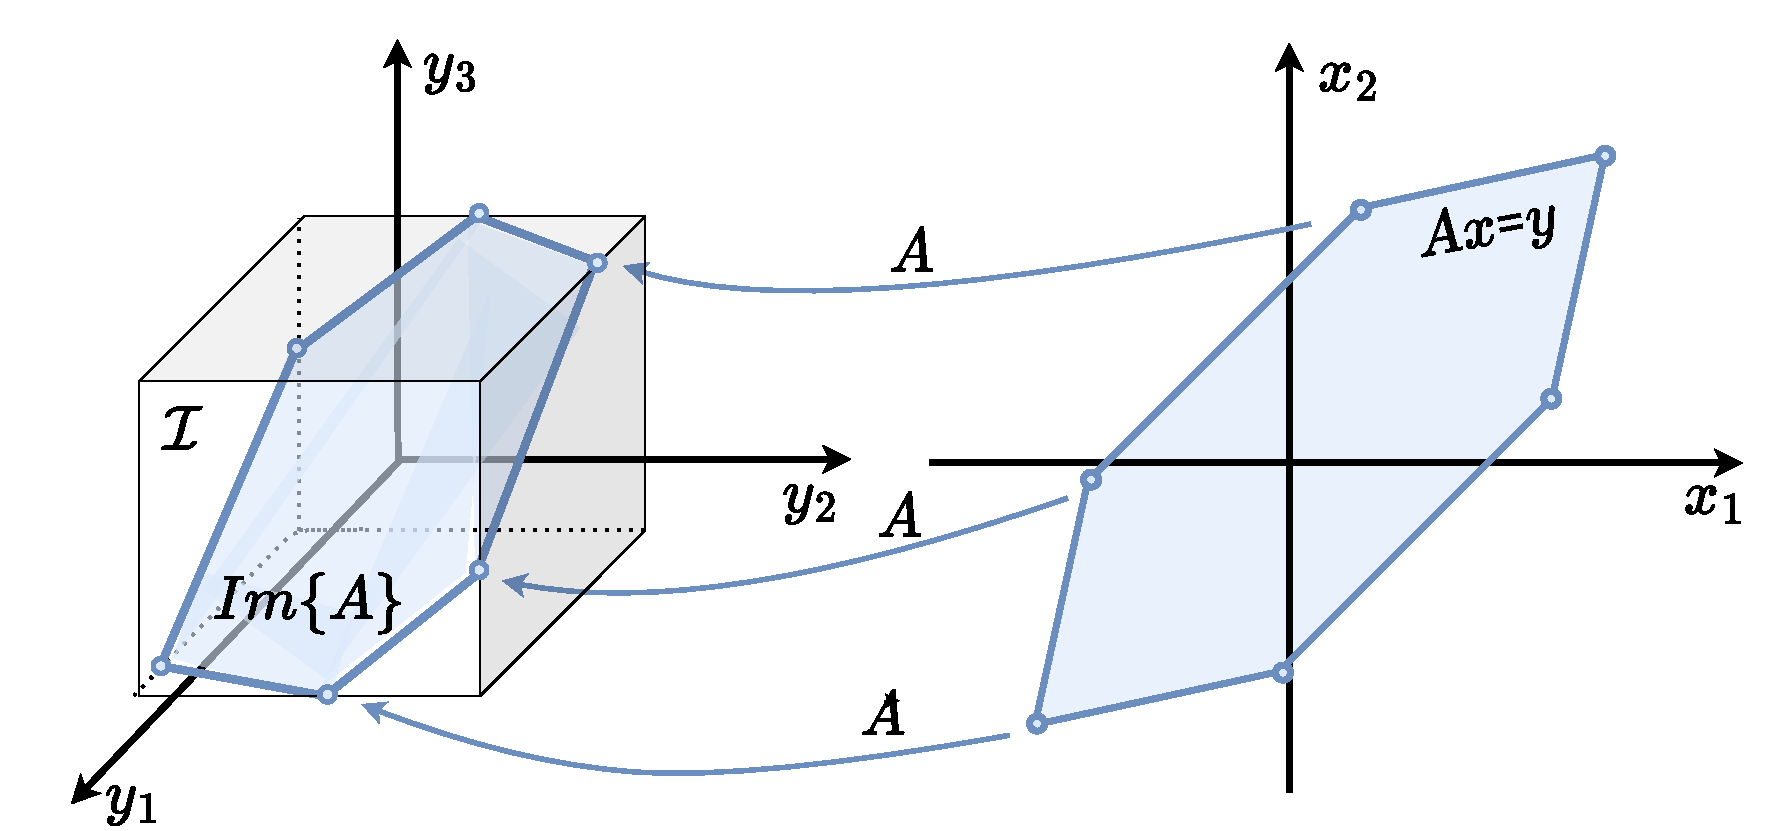
\includegraphics[width=0.8\linewidth]{Chapters/imgs/intersection.pdf}
    \caption{An example of the constructing an intersection formulation polytope with $m=2$ dimensional output space and $n=3$ dimensional input space. The intersection $\img{A} \cap \mathcal{I}_y$ of the hyperrectangle shaped input space $\mathcal{I}_y$ with the image of the matrix $A$ is shown in blue (left). This intersection can be projected to the output space using the inverse of the matrix $A$ to obtain the polytope $\mathcal{P}_x$ (blue right).}
    \label{fig:inter}
\end{figure}

The intersection polytope formulation (\ref{eq:inter_poly_revist}) with the interval limits 
\begin{equation}
    \mathcal{I}_y = \{ \bm{y}\in\mathbb{R}^n ~|~ \bm{y}\in[\bm{y}_{min},\bm{y}_{max}]\}
\end{equation}
is a spacial case of the intersection polytope formulation where the input space limits are defined as independent min-max ranges 
\begin{equation}
    \mathcal{P}_x=\{\bm{x}\in\mathbb{R}^m~ |~ A\bm{x} = \bm{y} + \bm{b}_y,~\bm{y}_{min} \leq  \bm{y} \leq \bm{y}_{max}  \}
    \label{eq:inter_hyp}
\end{equation}
\Cref{fig:inter} graphically represents the construction the polytope $\mathcal{P}_x$ from the input set $\mathcal{I}_y$.

When the input set has the interval form $\mathcal{I}_y$ the $\repr{H}$-representation of the polytope $\mathcal{P}_x$ can be found directly by substituting $\bm{y}$ with $A\bm{x}-\bm{b}_y$ in the interval equation $\bm{y}\in[\bm{y}_{min},\bm{y}_{max}]$ and rewriting it in the matrix from
\begin{equation}
   \underbrace{\begin{bmatrix}
        A\\
        -A
    \end{bmatrix}}_{H_x}\bm{x} \leq \underbrace{\begin{bmatrix}
         \bm{y}_{max} + \bm{b}_y\\
        -\bm{y}_{min} + \bm{b}_y 
    \end{bmatrix} }_{\bm{d}_x}
\end{equation}
where matrix $H_x\in\mathbb{R}^{2n \times m}$ and the vector $\bm{d}_x\in\mathbb{R}^{2n}$ can be used to express the $\repr{H}$-representation of the polytope $\mathcal{P}_x$
\begin{equation}
    \mathcal{P}_x=\{\bm{x}\in\mathbb{R}^m |~ H_x\bm{x} \leq \bm{d}_x \}
    \label{eq:inter_h_rep}
\end{equation}
However, as discussed at the beginning of \Cref{ch:inter_h_rep}, additional steps might be necessary to remove the redundant half-plane equations within the matrix $H_x$ and the vector $\bm{d}_x$.


\subsubsection{Finding the $\repr{V}$-representation} 
\label{ch:inter_v_rep}
Finding the $\repr{V}$-representation of polytopes with the intersection formulation, is a much more complex operation with respect to finding the $\repr{H}$-representation. 

In general, finding the $\repr{V}$-representation of the polytope $\mathcal{P}_x$, is performed by first finding its $\repr{H}$-representation, as described in the previous section (\Cref{ch:inter_h_rep}). Then, depending on the size of the problem, different standard representation conversion algorithms, described in \Cref{ch:standard_represtantion_conversion}, can be used to obtain its $\repr{V}$-representation.

However, as the special case of the intersection formulation, where the input set has interval shape $\mathcal{I}_y$, is particularly present in the robotics literature, several efficient algorithms have been proposed for finding its $\repr{V}$-representation directly.



\subsubsection*{Special case: Interval form $\mathcal{I}_y$}
\label{par:intersection_interval_algos_v}

When the input set has interval shape $\mathcal{I}_y$, the compact form of this polytope  $\mathcal{P}_x$ with the intersection formulation can be expressed as
\begin{equation}
    \mathcal{P}_x=\{\bm{x}\in\mathbb{R}^m ~ |~ A\bm{x} = \bm{y} + \bm{b}_y,~ \bm{y} \in [\bm{y}_{min},~  \bm{y}_{max}]  \}
    \label{eq:inter_hyp_revisit}
\end{equation}

Several efficient algorithms were developed for finding all the vertices of polytopes with this formulation. These algorithms, exploit the geometry of the problem and provide better efficiency than the standard conversion INA or GTA based methods.

An efficient algorithm for vertex enumeration of the intersection type polytope is proposed by \citet{gouttefarde_versatile_2015}. The algorithm assumes that the output space dimension is always $m=2$, in which case, the polytope $\mathcal{P}_x$ becomes a 2D polygon. The algorithm then exploits the 2D geometry of the problem and efficiently navigates the boundaries of the polygon in search for extremities. However, this algorithm does not scale well to higher dimensional problems.

A different algorithm, finding the $\repr{V}$-representation of the intersection polytope $\mathcal{P}_x$ with interval limits $\mathcal{I}_y$, is proposed by \citet{chiacchio_evaluation_1996}. The algorithm leverages the hyperrectangle geometry of the interval input set $\mathcal{I}_y$ and performs an efficient exhaustive search through its faces. This algorithm has been improved by \citet{sasaki2011vertex}, significantly reducing the computational complexity by exploiting the geometry of the intersection of the hyperrectangle (interval) $\mathcal{I}_y$ and the image of matrix $\img{A}$. Moreover, this improved algorithm is based on the equivalent projection formulation of the intersection polytope, described in the \Cref{par:equivalent_proj}.
\begin{equation}
\mathcal{P}_x=\{\bm{x}\in\mathbb{R}^m ~|~ \bm{x} = A^+\bm{y} + A^+\bm{b}_y,~ \bm{y} \in \img{A}\cap[\bm{y}_{min},\bm{y}_{max}]\}
\label{eq:inter_hyp_inter}
\end{equation}

Both of these algorithms, \citet{chiacchio_evaluation_1996} and \citet{sasaki2011vertex}, are based on the efficient exhaustive search of the hyperrectangle $\mathcal{I}_y$ faces. However, the number of faces of the hyperrectangle grows exponentially with the input space dimension
$$
N_{n,k}= 2^{n-k}\binom{n}{k}
$$
where $n$ is the dimension of the input space, $N_{n,k}$ is the number of the $k$ dimensional hyperrectangle faces. Therefore,  as the dimension of the input space $n$ grows, the computational efficiency of these algorithms decreases exponentially.

\subsection{Strategies for the projection formulation}
\label{ch:projection_algos}

This section brings a short overview of methods used for the transformation of polytopes with projection formulation, described in \Cref{ch:proj_formulaiton}, into their respective $\repr{V}$ and $\repr{H}$-representation.

\label{ch:proj_poly_chapter}
\begin{figure}
    \centering
    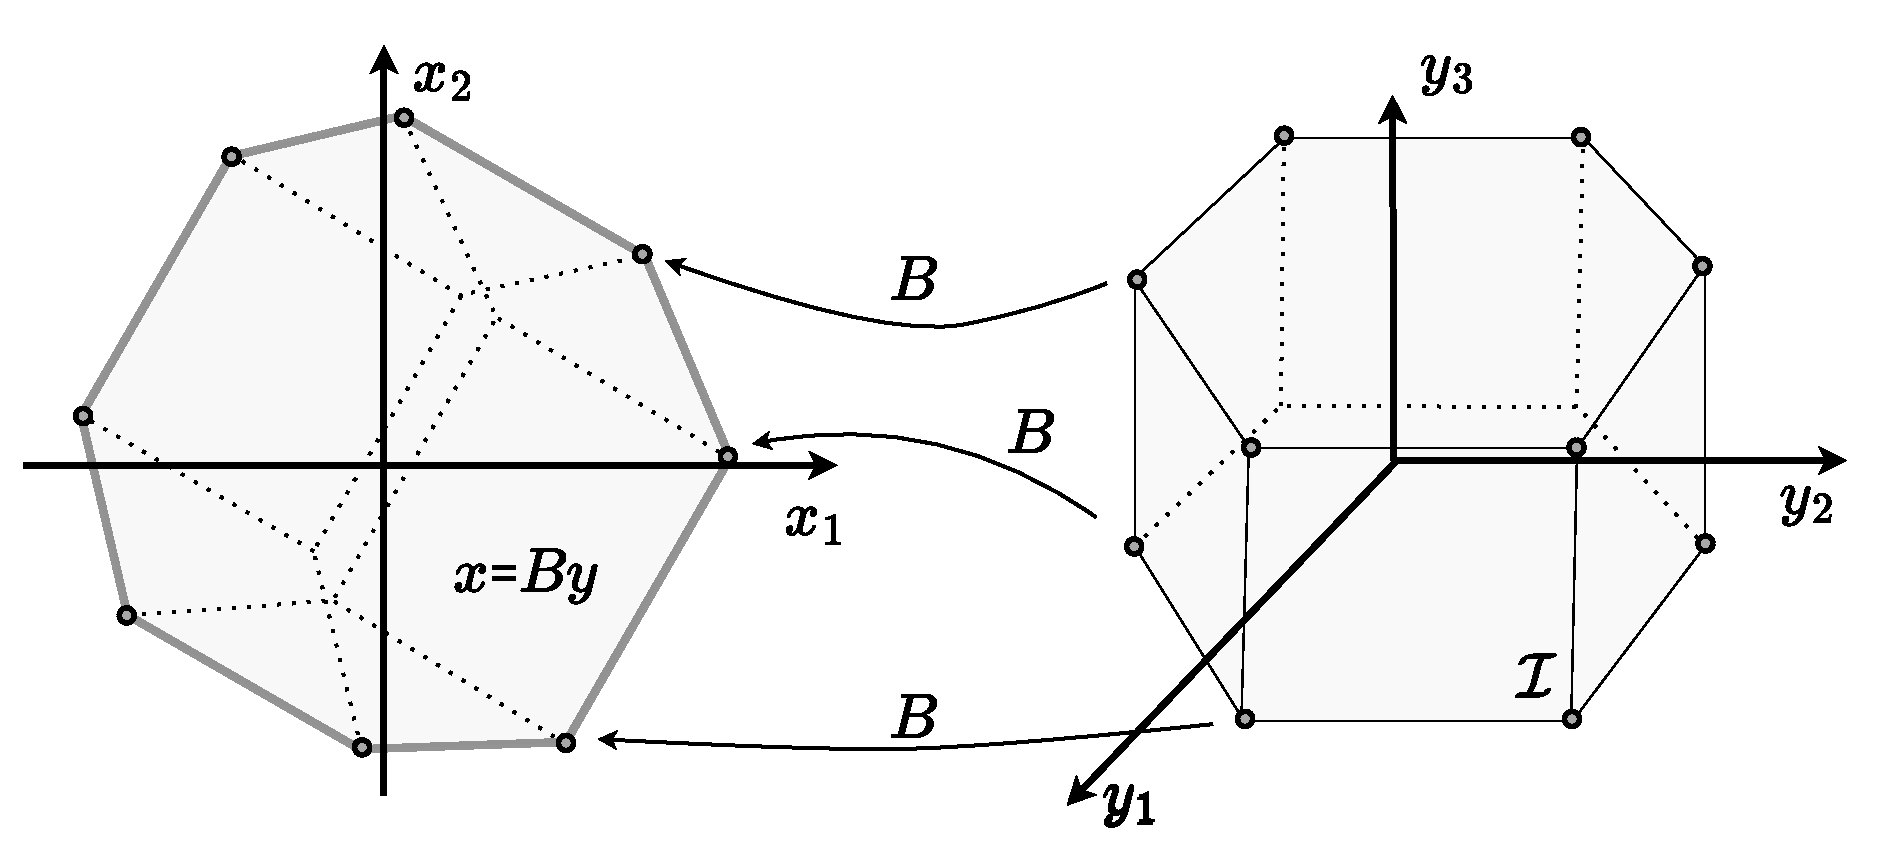
\includegraphics[width=0.7\linewidth]{Chapters/imgs/proj_poly.pdf}
    \caption{An example of the constructing a projection formulation polytope with $m=2$ dimensional output space and $n=3$ dimensional input space, where the input space $\mathcal{P}_y$ has a polytope shape. In this formulation, the whole input space $\mathcal{P}_y$ (grey) is projected using the matrix $B$ to the output space to obtain the polytope $\mathcal{P}_x$ (blue). }
    \label{fig:proj_poly}
\end{figure}

The projection polytope (\ref{eq:proj_poly}) with polytope input set $\mathcal{P}_y$ can be expressed as
\begin{equation}
    \mathcal{P}_x=\{\bm{x}\in\mathbb{R}^m |~ \bm{x} = B\bm{y} + \bm{b}_x,~\bm{y} \in \mathcal{P}_y  \}
    \label{eq:proj_poly_1}
\end{equation}
where $\bm{y}\in\mathbb{R}^n$ is an $n$ dimensional input vector, $\bm{x},\bm{b}_x\in\mathbb{R}^m$ are the $m$ dimensional output vector and bias, while $B\in\mathbb{R}^{m\times n}$ is a transformation matrix from input to the output space.

The geometrical representation of the polytope $\mathcal{P}_x$ defined by (\ref{eq:proj_poly_1}) is shown on \Cref{fig:proj_poly}, for the example of $n=3$ dimensional polytope $\mathcal{P}_y$ and $m=2$ dimensional polytope $\mathcal{P}_x$. The resulting polytope $\mathcal{P}_x$ is an affine projection of the input polytope $\mathcal{P}_y$ into the lower dimensional output space. Furthermore, the vertices and the faces of the polytope $\mathcal{P}_x$ correspond to the subset of the projected vertices and faces of the input polytope $\mathcal{P}_y$. 

Given the structure of the input set $\mathcal{P}_y$ algorithms for finding the $\repr{V}$ and $\repr{H}$-representation vary in complexity. 

\subsubsection{Finding the $\repr{V}$-representation}
\label{ch:proj_algos_v}
If the input set polytope $\mathcal{P}_y$ is expressed using its vertex or $\repr{V}$-representation
\begin{equation}
    \mathcal{P}_y = \conv{ \bm{y}_{v1}, ~ \bm{y}_{v2},~ \ldots}
    \label{eq:proj_v_step1}
\end{equation}
where $\bm{y}_{vi}\in\mathbb{R}^n$ are the vertices of the polytope $\mathcal{P}_y$, the vertices of the projection formulation polytope (\ref{eq:proj_poly_1}) can then be found by projecting the vertices of $\mathcal{P}_y$ to the output space using the matrix $B \in \mathbb{R}^{m\times n}$ and calculating their Convex-Hull $\conv{\cdot}$
\begin{equation}
    \mathcal{P}_x= \conv{ B\bm{y}_{v1}, ~ B\bm{y}_{v2},~ \ldots}
    \label{eq:proj_v_step2}
\end{equation}
The Convex-Hull algorithm finds the $\repr{V}$-representation of the projection polytope directly, as the vertices of the polytope $\mathcal{P}_x$ are a subset of the projected vertices $\bm{y}_{vi}$ of the input polytope $\mathcal{P}_y$, as shown in the example on \Cref{fig:proj_poly}. 

If the input polytope $\mathcal{P}_y$ is expressed using its half-plane or $\repr{H}$-representation, 
\begin{equation}
    \mathcal{P}_y = \{ \bm{y}\in\mathbb{R}^n ~|~H_y\bm{y} \leq \bm{d}_y\}
\end{equation}
there are two main approaches decoupling the problem.

The first and straight-forward approach consists in finding the $\repr{V}$-representation of the input set $\mathcal{P}_y$ first, using the standard representation conversion methods described in \Cref{ch:standard_represtantion_conversion}. Then the above described procedure (\ref{eq:proj_v_step1}-\ref{eq:proj_v_step2}) can be used to find the $\repr{V}$-representation of  $\mathcal{P}_x$. However, in many cases, when the input space dimension $n$ is high or if the geometry of the polytope  $\mathcal{P}_y$ is complex (large number of faces and vertices), finding its $\repr{V}$-representation might be computationally demanding. 

The second approach, more efficient in many cases, consists in finding the $\repr{H}$-representation of the polytope $\mathcal{P}_x$ directly from the input set's $\repr{H}$-representation. One of the most well known algorithms for projecting the $\repr{H}$-representation of polytopes is arguably the \gls{fme} described by \citet{dantzig1973fourier}.  This algorithm uses an iterative inequality elimination method to isolate the set of half-plane equations bounding the final polytope $\mathcal{P}_x$. However, this approach has an exponential complexity with the dimension of the input space $n$ \cite{Talaashrafi2020complexity}, and additionally it does not guarantee a minimal representation \cite{Monniaux2010}. A more efficient algorithm is introduced by \citet{jones2004equality} called \gls{esp}. As opposed to \gls{fme}, this algorithm is \textit{output sensitive}, having its execution time proportional to the complexity of the final polytope $\mathcal{P}_x$ (it number of faces and vertices), making it particularly well suited to the high dimensional input spaces $\mathbb{R}^n$. A more in depth comparison of these methods, as well their comparison to several other polytope projection algorithms, is brought in the work by \citet{Gl_le_2018}. Once the $\repr{H}$-representation of the polytope $\mathcal{P}_x$ is obtained using one of these methods, the standard representation conversion methods can be used to obtain the $\repr{V}$-representation of the polytope $\mathcal{P}_x$ defined in the $m$ dimensional output space.

The same two approaches can be used in the general case, where the input set $\mathcal{P}_y$ does not correspond neither to the $\repr{V}$ nor to the $\repr{H}$-representation. The choice of the more suitable one depends on the efficiency of transforming the input set $\mathcal{P}_y$ into its $\repr{V}$ or $\repr{H}$-representation. 

In remaining part of this section three special cases of the input set formulation are discussed: intersection and projection formulation of the input set $\mathcal{P}_y$, as well as the interval form $\mathcal{I}_y$.

\subsubsection*{Special case: intersection formulation} If the input set $\mathcal{P}_y$ has the intersection formulation, then the formulation of the polytope $\mathcal{P}_x$ corresponds to the projection-intersection formulation, the combined special case  described in \Cref{ch:proj_inter_form}.

The $\repr{H}$ and $\repr{V}$-representations of the input set $\mathcal{P}_y$, with intersection formulation, can be obtained using the strategies discussed in \Cref{ch:intersection_algos}. As discussed in \Cref{ch:intersection_algos}, in general, the $\repr{H}$-representation of intersection polytopes can be found more efficiently than the $\repr{V}$-representation, making the second approach described in \Cref{ch:proj_algos_v} better suited.


\subsubsection*{Special case: projection formulation} 
If the input set $\mathcal{P}_y$ has the projection formulation itself
\begin{equation}
    \mathcal{P}_y=\{\bm{y}\in  \mathbb{R}^n~|~ \bm{y}=D\bm{z} + \bm{b}_y, ~ \bm{z} \in \mathcal{P}_z \}
\end{equation}
where $\bm{z}\in\mathcal{R}^k$ is its $k$ dimensional input vector, bounded within the set $\mathcal{P}_z$, $\bm{b}_y\in\mathbb{R}^n$ is the bias vector, and the matrix $D\in \mathbb{R}^{n\times k}$ is a projection matrix form the $k$ dimensional space to the $n$ dimensional space.

Then the two projection formulations can be combined into the new polytope $\mathcal{P}_x$, by replacing the $\bm{y}$ with $D\bm{z} + \bm{b}_y$ in initial formulation of $\mathcal{P}_x$ (\ref{eq:proj_poly_1}).
\begin{equation}
    \mathcal{P}_x=\{\bm{x}\in  \mathbb{R}^m~|~ \bm{x}=\underbrace{BD}_{B'}\bm{z} + \underbrace{B\bm{b}_z + \bm{b}_x}_{\bm{b}_x'}, ~ \bm{z} \in \mathcal{P}_z \}
\end{equation}
This new formulation corresponds to the projection formulation as well. Therefore, the same approaches described in \Cref{ch:proj_algos_v} can be used to find its $\repr{V}$-representation respectively.

\subsubsection*{Special case: Interval form $\mathcal{I}_y$} 


\begin{figure}
    \centering
    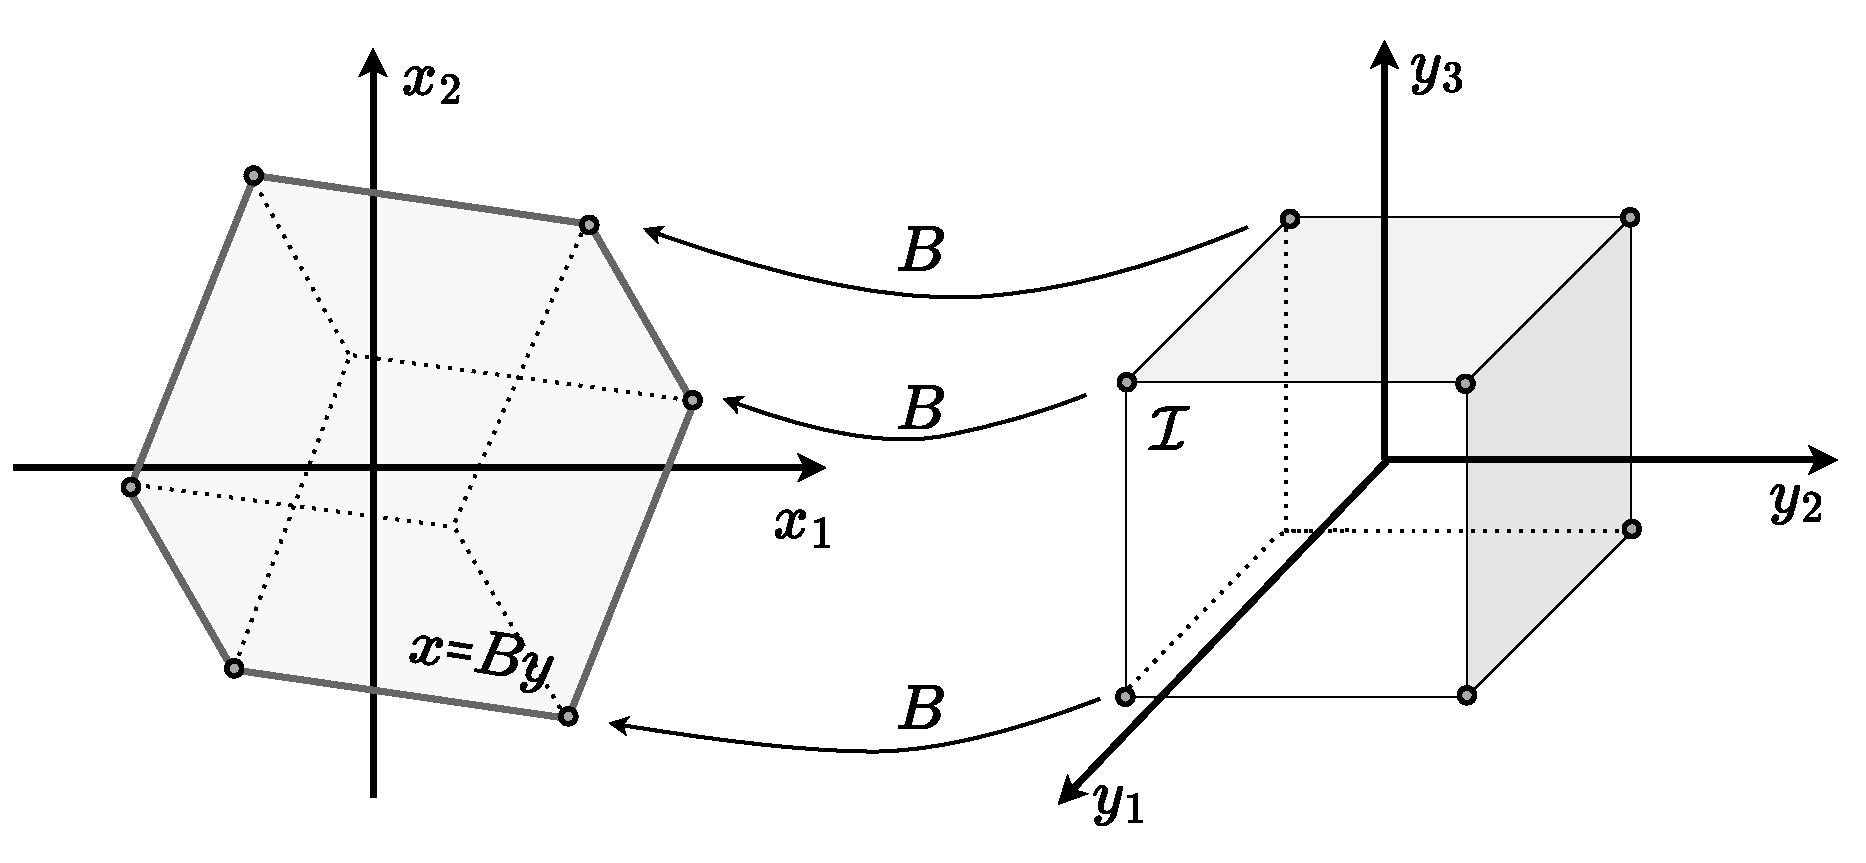
\includegraphics[width=0.8\linewidth]{Chapters/imgs/projection.pdf}
    \caption{An example of the constructing a projection formulation polytope with $m=2$ dimensional output space and $n=3$ dimensional input space, where the input space $\mathcal{I}_y$ has a hyperrectangle (interval) shape. In the projection formulation, the whole input space $\mathcal{I}_y$ (grey) is projected using the matrix $B$ to the output space to obtain the polytope $\mathcal{P}_x$ (blue). }
    \label{fig:proj}
\end{figure}

The projection polytope formulation $\mathcal{P}_x$ with the interval limits $\mathcal{I}_y$
\begin{equation}
    \mathcal{I}_y = \{ \bm{y}\in\mathbb{R}^n ~|~ \bm{y}\in[\bm{y}_{min},\bm{y}_{max}]\}
\end{equation}
is a spacial case of the projection polytope formulation which can be compactly expressed as
\begin{equation}
    \mathcal{P}_x=\{\bm{x}\in\mathbb{R}^m |~ \bm{x} = B\bm{y} + \bm{b}_x,~\bm{y}_{min} \leq  \bm{y} \leq \bm{y}_{max}  \}
    \label{eq:proj_hyp}
\end{equation}
\Cref{fig:proj} graphically represents the construction the polytope $\mathcal{P}_x$ from the input set $\mathcal{I}_y$.

The most straight-forward way of finding the vertices $\bm{x}_{vi}\in\mathbb{R}^m$ of the projection polytope $\mathcal{P}_x$ is by first enumerating the $2^n$ vertices $\bm{y}_{vi}\in\mathbb{R}^n$ of the hyperrectangle  (interval) $\mathcal{I}_y$, by creating a list of all the combinations of the minimal $\bm{y}_{min}$ and maximal $\bm{y}_{max}$ values of $\bm{y}$
\begin{equation}
    \bm{y}_{v1} = \begin{bmatrix}
        y_{1,min}\\
        y_{2,min}\\
        \ldots\\
        y_{n,min}\\
    \end{bmatrix},\quad
    \bm{y}_{v2} = \begin{bmatrix}
        y_{1,max}\\
        y_{2,min}\\
        \ldots\\
        y_{n,min}\\
    \end{bmatrix},\qquad\ldots,\qquad
    \bm{y}_{v2^n} = \begin{bmatrix}
        y_{1,max}\\
        y_{2,max}\\
        \ldots\\
        y_{n,max}\\
    \end{bmatrix} 
\end{equation}
Then these vertices can be projected to the lower dimensional output space $\mathbb{R}^m$ using the projection matrix $B\in \mathbb{R}^{m\times n}$, where the polytope $\mathcal{P}_x$ can be found by calculating the Convex-Hull $\conv{\cdot}$ of the projected points.
\begin{equation}
    \mathcal{P}_x = \conv{B\bm{y}_{v1},B\bm{y}_{v2},~\ldots, ~ B\bm{y}_{v2^n}}
\end{equation}

The complexity of this approach depends on two factors. The dimension of the of the input space $n$ and the dimension of the output space $m$. The number of vertices of the hyperrectangle (interval) grows exponentially ($2^n$) with the dimension of the input space $n$, and constructing a matrix of $2^n \times n$ entries can become impractical. On the other hand, as this approach requires a Convex-Hull algorithms, which are executed in the $m$-dimensional output space, the dimension $m$ might make the Convex-Hull algorithm impractical as their complexity grows significantly with the dimension of the space $m$ \cite{Barber1996}.

Therefore for higher dimensional output spaces (typically $m\geq 4$) and input spaces (causing the memory issues due to  $2^n \times n$ matrix construction) a more efficient approach might be to first calculate the $\repr{H}$-representation of this polytope, using the methods described in the following section, and then use standard representation conversion methods (\Cref{ch:standard_represtantion_conversion}), to find its $\repr{V}$-representation.


\subsubsection{Finding the $\repr{H}$-representation}
\label{ch:proj_algos_h}

If the input polytope $\mathcal{P}_y$ is expressed using its half-plane or $\repr{H}$-representation, 
\begin{equation}
    \mathcal{P}_y = \{ \bm{y}\in\mathbb{R}^n ~|~H_y\bm{y} \leq \bm{d}_y\}
\end{equation}
the straight-forward approach consists in decoupling the problem and find the $\repr{V}$-representation first, using the standard representation conversion methods  described in \Cref{ch:standard_represtantion_conversion}, then follow the above described procedure (\Cref{ch:proj_algos_v}) to find the $\repr{V}$-representation of $\mathcal{P}_x$. 

As described in the previous section, in many cases, when the input space dimension $n$ is high or if the geometry of the polytope  $\mathcal{P}_y$ is complex (large number of faces and vertices), finding its $\repr{V}$-representation might be computationally demanding. In those cases, if the $\repr{H}$-representation of the polytope $\mathcal{P}_y$ is available, the $\repr{H}$-representation of the polytope $\mathcal{P}_x$ can be found directly using the algorithms such as \gls{fme} and \gls{esp}. 

These same two approaches can be used in the general case, where the input set $\mathcal{P}_y$ does not correspond neither to the $\repr{V}$ nor to the $\repr{H}$-representation. The choice of the more suitable one depends on the efficiency of transforming the input set $\mathcal{P}_y$ into its $\repr{V}$ or $\repr{H}$-representation. 

\subsubsection*{Special case: Interval form $\mathcal{I}_y$} 

The projection polytope formulation $\mathcal{P}_x$ with the interval limits $\mathcal{I}_y$ can be compactly expressed
\begin{equation}
    \mathcal{P}_x=\{\bm{x}\in\mathbb{R}^m |~ \bm{x} = B\bm{y} + \bm{b}_x,~\bm{y}_{min} \leq  \bm{y} \leq \bm{y}_{max}  \}
    \label{eq:proj_hyp_1}
\end{equation}

Apart from the two approaches described at the beginning of this section (\Cref{ch:proj_algos_h}), there are several more efficient algorithms introduced in the literature, specific for this formulation and typically exploiting the polytope's zonotope structure.

One such  efficient algorithm, exploiting the geometry of the formulation (\ref{eq:proj_hyp_1}) of the projection polytope $\mathcal{P}_x$ with interval limits $\mathcal{I}_y$, is introduced by \citet{Bouchard2009} and improved by Gouttefarde and Krut \cite{hyper_psm}. It is often referred to as \gls{hpsm}. This algorithm finds the minimal $\repr{H}$-representation of the polytope (\ref{eq:proj_hyp_1}) by efficiently performing the exhaustive search of all the possible half-plane combinations corresponding to the $m-1$ dimensional polytope $\mathcal{P}_x$ faces. Even-though much more efficient than the \glsxtrfull{fme}, this algorithm still has considerable (binomial) complexity, as it relies on the exhaustive search in the $n$ dimensional input space where the number $N_h$ of hyper-planes to be tested equals to 
$$N_h = \binom{n}{m-1}$$

\subsection{Polytope approximation strategies}
\label{ch:approximation_algos}

Exact vertex and facet enumeration methods, such as the standard representation conversion methods described in \Cref{ch:standard_represtantion_conversion} or more specific methods for the projection and the intersection formulation described in \Cref{ch:intersection_algos} and \Cref{ch:projection_algos}, rely on different versions of exhaustive search in the $n$-dimensional input space, which is often higher dimensional than the output space $n> m$. Their execution time is typically exponential, or polynomial in the best case, with respect to the dimension of the input space $n$, the number of vertices and the faces of the input set $\mathcal{P}_y$ and the final polytope $\mathcal{P}_x$ \cite{Dyer1983}. Therefore, in cases where the input space is much higher dimensional than the output space $n\gg m$ or when the polytopes $\mathcal{P}_x$ and $\mathcal{P}_y$ have complex geometries (large number of faces and vertices), such approaches may not be practically viable for interactive, in-the-loop, applications. 

To overcome this issue, various approximate approaches, such as the \gls{rsm} \cite{agarwal1993ray} and the \gls{chm} \cite{lassez1992quantifier} have been developed, reducing the complexity and improving the execution time. 

\begin{wrapfigure}{r}{0.35\linewidth}
% \vspace{-0.5cm}
% \begin{framed}
    \centering
    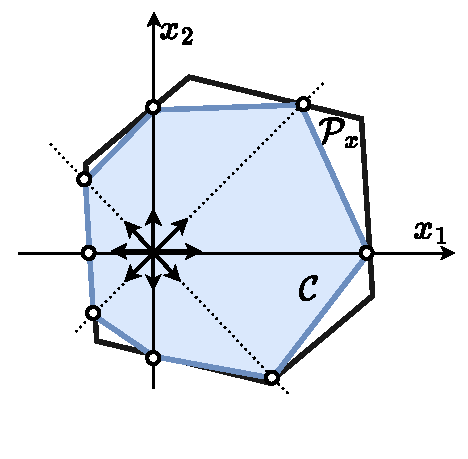
\includegraphics[width=\linewidth]{Papers/images/rsm.pdf}
    \caption{An example of the approximation $\mathcal{C}$ of the 2D ($m\!=\!2$) polytope $\mathcal{P}_x$ using a \gls{rsm} algorithm. The input space is sampled with 8 rays. }
    \label{fig:rsm}
% \end{framed}
\end{wrapfigure}
The \gls{rsm} algorithms are relatively simple to setup as they rely on different forms of sampling (shooting rays) of the polytope $\mathcal{P}_x$, in the low dimensional output space. Their execution time is proportional to the number of sampling directions (rays shot), therefore, by choosing an appropriate sampling strategy, the \gls{rsm} algorithms can provide an efficient approximation of the polytope $\mathcal{P}_x$. However, these algorithms do not provide any bound on their estimation error and rely highly on hand tuned initial parameters. \Cref{fig:rsm} shows a visual example of a \gls{rsm} approximation of a polygon $\mathcal{P}_x$ using uniform sampling in the output space with 8 rays.

The \gls{chm} algorithms, first introduced by \citet{lassez1992quantifier, Huynh2005PracticalIO}, propose an efficient iterative approximation of the polytope $\mathcal{P}_x$, while at the same time avoiding the complexity of the exhaustive search. The CHM algorithms simplify the final polytope $\mathcal{P}_x$ geometry by removing the need to find all the faces and vertices of the polytope. Such algorithms are usually defined in the lower-dimensional output space $\bm{x}\in \mathbb{R}^m$ making them \textit{output sensitive}, having the execution time proportional to the number of vertices and the faces of the output space polytope $\mathcal{P}_x$. In addition to searching in the lower $m$ dimensional output space, they enable finding an efficient inner (or outer) approximation of the polytope $\mathcal{P}_x$, while satisfying a user defined level of accuracy. Finally, they find both the vertices and the faces of the polytope $\mathcal{P}_x$ at the same time, providing both $\repr{V}$ and the $\repr{H}$-representation \cite{Gl_le_2018}.


The execution of a typical \gls{chm} algorithm consists in two phases. In the first phase an initial approximation of the polytope $\mathcal{P}_x$ is constructed finding a subset of $m+1$ vertices forming an initial $m$-dimensional Convex-Hull $\mathcal{C}$ approximation of the polytope $\mathcal{P}_x$. In the second phase, the Convex-Hull approximation $\mathcal{C}$ is refined iteratively until the desired accuracy is reached. The \gls{chm} algorithms use a sequence of \glspl{lp} to find new vertices of the polytope in each iteration, followed by the Convex-Hull algorithm to group them to the faces. An example of the \gls{chm} algorithm iterations for $m=2$ output space is shown on \Cref{fig:chm}.   

The \gls{chm} algorithms have several limitations though. The resolution of the algorithms relies on the iterative application of the Convex-Hull algorithm which complexity grows exponentially for output space dimensions $m > 3$ \cite{Barber1996}. As a result, the applications of these methods have so far been limited to the low-dimensional output spaces $m\leq3$. Additionally, as different polytope formulations require different \gls{lp} formulations, the implementations of these methods are often somewhat specific to their respective applications. 

There are several examples in the literature where the approximation based methods were used for improving the efficiency of different computationally expensive polytope evaluation problems. \citet{Bretl2008} have proposed a \gls{chm} based algorithm for approximating 2D ($m\!=\!2$) polytopes in the context of legged robot locomotion. \citet{DelPrete2016Fast} recently proposed an efficiency improvement of this algorithm, and \citet{Herve2018} extended it to the 3D ($m\!=\!3$) use-cases. This algorithm calculates the inner and outer approximation of the polytope $\mathcal{P}_x$ at the same time, while its accuracy condition can be set a as desired ratio between the inner and outer approximation volumes. \citet{Ponce1995} have introduced a derivative of the \gls{chm} algorithm to calculate the 2D, 3D and 4D ($m\!=\!2,3,4$) polytopes in the context of grasping objects with multiple fingers. While \citet{Xu2008projection} used a \gls{chm} algorithm in the context in the context of information theory. Both of these algorithms find all vertices and faces of the output polytope $\mathcal{P}_x$, without exploiting \gls{chm}'s approximation capacity. Furthermore, \citet{carmichael_estimating_2013,carmichael2011Towards} used an \gls{rsm} algorithm for approximating 2D and 3D ($m\! =\! 2,3$) polytopes in the context of human force capacity estimation, based on a musculoskeletal model. In order to enable real-time execution, their \gls{rsm} implementation relies on the uniform sampling in the output space.

 
\begin{figure}
    \centering
    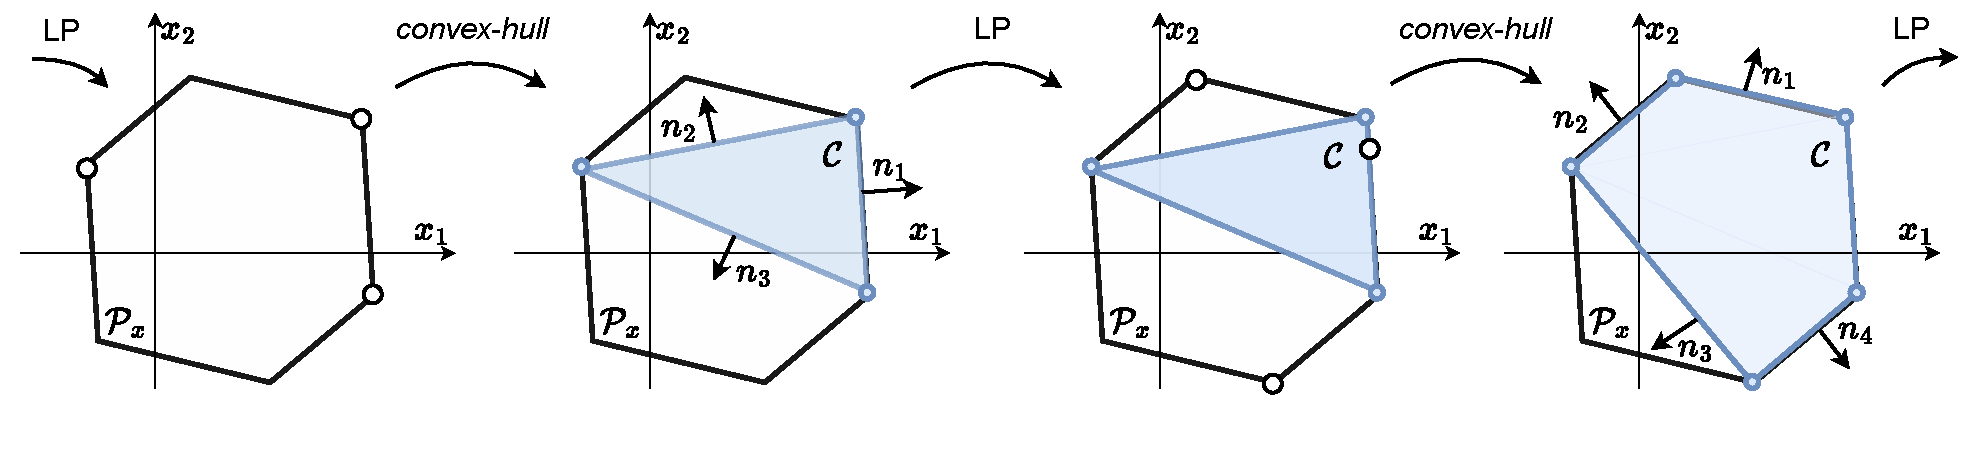
\includegraphics[width=\linewidth]{Papers/images/chm_algo.pdf}
    \caption{This figure shows the procedure of successive approximation of the polytope $\mathcal{P}_x$ using the \gls{chm} algorithm. The face normal vectors $\bm{n}_i$ of the Convex-Hull $\mathcal{C}$ are used with \gls{lp} to find new vertices which are then used to update the Convex-Hull $\mathcal{C}$ and furthermore improve the approximation of the polytope.}
    \label{fig:chm}
\end{figure}

In summary, when the complexity of the polytope $\mathcal{P}_x$ transformation does not permit using standard exact methods in the practical applications, especially when the dimension $n$ of the input space is high while the dimension of the output space $m$ is reasonably low $m\leq3$, polytope approximation methods, such as \gls{rsm} and \gls{chm} algorithms, provide a more efficient solutions. The \gls{rsm} algorithms provide a fast sampling based approximation, however without any guarantees on the approximation error or accuracy. On the other hand, \gls{chm} algorithms use an efficient iterative approach to the polytope approximation, while at the same time being capable of guaranteeing the maximal approximation error.

\subsection{Synthesis of transformation strategies}
\label{ch:overview_algo_synthesis}
\afterpage{
\begin{landscape}
\vspace*{\fill}
\begin{table}[!h]
    \hspace{-2cm}   
    \scalefont{0.85}
    \centering
    \begin{tabular}{|l|c|c|c|c|c|c|c|c|c|c|c|c|c|c|c|c|c|c|}
    \hline
         Formulation & \multicolumn{2}{c|}{ \begin{tabular}{@{}c@{}@{}} Generic (Unified) \\ $A \bm{x}=B\bm{y} + \bm{b}$, $\bm{y}\in \mathcal{P}_y$ \\ \Cref{eq:generic_polyt_view_revisit}\end{tabular}} &\multicolumn{8}{c|}{ \begin{tabular}{@{}c@{}@{}}Projection (Proj.) \\ $ \bm{x}=B\bm{y} + \bm{b}_x$, $\bm{y}\in \mathcal{P}_y$ \\ \Cref{eq:proj_poly}
         \end{tabular}} & \multicolumn{8}{c|}{\begin{tabular}{@{}c@{}@{}}Intersection (Int.)\\ $ A\bm{x}=\bm{y} + \bm{b}_y$, $\bm{y}\in \mathcal{P}_y$ \\ {\Cref{eq:inter_poly}}\end{tabular}} \\
    \hline
         \begin{tabular}{@{}l@{}}Finding \\ representation\end{tabular} &
         \hspace*{0.5cm}$\repr{H}$\hspace*{0.5cm} & $\repr{V}$ & \multicolumn{3}{c|}{$\repr{H}$}& \multicolumn{5}{c|}{$\repr{V}$}& \multicolumn{3}{c|}{$\repr{V}$}& \multicolumn{5}{c|}{$\repr{H}$}\\
    \hline
        \begin{tabular}{@{}l@{}}Input set $\mathcal{P}_y$ \\ special cases \end{tabular} &
        \multicolumn{2}{c|}{-}
        & $\mathcal{I}_y$& $\repr{H}_y$ & other&  $\mathcal{I}_y$& Proj. &   $\repr{V}_y$ & Int. &other & $\mathcal{I}_y$& other & $\repr{H}_y$  & Int. & $\mathcal{I}_y$ & $\mathcal{H}_y$ & Proj. & other \\
    \hline
    \multicolumn{1}{c}{}&\multicolumn{18}{c}{State of the art resolution strategies}\\
    \hline
         \begin{tabular}{@{}l@{}}Overview\\ Section \end{tabular} &
        \multicolumn{2}{c|}{-} &
        \multicolumn{3}{c|}{ \Cref{ch:proj_algos_h} }& \multicolumn{5}{c|}{\Cref{ch:proj_algos_v}}& \multicolumn{3}{c|}{\Cref{ch:inter_v_rep}}& \multicolumn{5}{c|}{\Cref{ch:inter_h_rep}}\\
    \hline
        \begin{tabular}{@{}l@{}}Standard exact \\ Methods\end{tabular} &
        \multicolumn{2}{c|}{N/A}
        &HPSM \cite{hyper_psm}& \begin{tabular}{@{}c@{}}FME \cite{dantzig1973fourier}, \\ ESP \cite{jones2004equality}\end{tabular}
        & N/A & \multicolumn{3}{c|}{ \begin{tabular}{@{}c@{}@{}}\Cref{ch:standard_represtantion_conversion} \\ ex. DDM \cite{fukuda_dd} \end{tabular} } & \multicolumn{2}{c|}{ N/A } & \begin{tabular}{@{}c@{}}Chiacchio \cite{chiacchio_evaluation_1996}, \\Sasaki \cite{sasaki2011vertex}\end{tabular} & N/A &  \multicolumn{4}{c|}{  \begin{tabular}{@{}c@{}@{}}\Cref{ch:standard_represtantion_conversion} \\ ex. DDM \cite{fukuda_dd} \end{tabular} } & \multicolumn{2}{c|}{ N/A } \\
    \hline
         \begin{tabular}{@{}l@{}}Approximation \\ Methods\end{tabular} & \multicolumn{2}{c|}{
         RSM \cite{carmichael_estimating_2013}}
         & \multicolumn{16}{c|}{\Cref{ch:approximation_algos}} \\
    \hline
    \multicolumn{1}{c}{}&\multicolumn{18}{c}{Proposed algorithms}\\
    \hline
         \begin{tabular}{@{}l@{}}VEPOLI$^2$ \\ \Cref{sec:algorithm_vea}\end{tabular} & \multicolumn{10}{c|}{ } 
         & \cellcolor{red!25} VEPOLI$^2$ &
         \multicolumn{7}{c|}{ } \\
    \hline
         \begin{tabular}{@{}l@{}}ICHM \\ \Cref{ch:algorihtm_ichm}\end{tabular} & \multicolumn{18}{c|}{\cellcolor{red!25}ICHM} \\
    \hline
    \end{tabular}
    \caption{This table brings a condensed view of the overview of the standard polytope evaluation methods applicable to different polytope formulations. The table brings methods for projection and intersection formulations and their generic unified form. As described in the overview different standard methods are often defined for finding $\repr{H}$ or $\repr{V}$-representation for one of the polytope formulations. Furthermore, the methods are often specific to one spacial case of the input set $\mathcal{P}_y$: they might require its Interval $\mathcal{I}_y$, Projection (Proj.) or Intersection (Int.) form, or in some cases its half-plane and vertex representation $\repr{H}_y$ or $\repr{V}_y$.
    The table shows that there are several cases where the standard methods are not directly applicable (N/A), but might require a sequence of several methods in order to be evaluated. The table also shows the applicability (red cells) of the algorithms VEPOLI$^2$ and ICHM introduced in \Cref{sec:algorithm_vea} and \Cref{ch:algorihtm_ichm} respectively.}
    \label{tab:algorithms table}
\end{table}
\vspace*{\fill}
\end{landscape}
}


\Cref{ch:polytope_algorithms} brings an overview of the standard polytope evaluation strategies applicable to finding the $\repr{H}$ and $\repr{V}$-representation of polytopes with the projection and the intersection formulation. For each one of the formulations, several special cases of the input space $\mathcal{P}_y$ are considered and the appropriate methods are described. 
The overview proposes both standard exact polytope evaluation methods (\Cref{ch:standard_represtantion_conversion,ch:intersection_algos,ch:projection_algos}) and polytope approximation methods (\Cref{ch:approximation_algos}). Additionally, a brief discussion on their computational complexity is given as well. 

The aim of this overview is to serve as a guide for finding an appropriate polytope evaluation strategy given the polytope $\mathcal{P}_x$ formulation, the shape of the input set $\mathcal{P}_y$ and provide an insight into their time-efficiency. 
As a visual tool, this section proposes a condensed view of the overview in the form of \Cref{tab:algorithms table}. The table groups the discussed state of the art methods with respect to their direct applicability to different evaluation cases. 
If the polytope evaluation case does not have any method directly applicable, it is denoted with N/A (Not Applicable). 

The table demonstrates that there are several polytope evaluation cases where the standard exact methods are not directly applicable, or potentially require several methods used sequentially. On the other hand, the approximation methods are applicable to the transformation of both the intersection and the projection formulations. Moreover, in the case of the generic formulation (\ref{eq:generic_polyt_view_revisit}), to the best of our knowledge, only the \gls{rsm} method by \citet{carmichael_estimating_2013} has been applied.

The following two sections introduce two new polytope evaluation algorithms called VEPOLI$^2$ (\Cref{sec:algorithm_vea}) and ICHM (\Cref{ch:algorihtm_ichm}). Both algorithms are added to \Cref{tab:algorithms table}, showing their applicability to different polytope evaluation problems. 


\section{VEPOLI$^2$: New vertex finding algorithm for intersection formulation}
\label{sec:algorithm_vea}

One typical example of the polytope with the intersection formulation (\ref{eq:inter_poly}) and interval input set (\ref{eq:hypercube_lim}) is the feasible wrench polytope, discussed in \Cref{ch:poly_force},
\begin{equation}
    \mathcal{P}_f(\bm{q},\dot{\bm{q}},\ddot{\bm{q}}) = \left\{ \bm{f} \in \mathbb{R}^m ~|~ \bm{\tau}\in\left[\bm{\tau}_{min}, \bm{\tau}_{max} \right], ~~ J^T(\bm{q})\bm{f} = \bm{\tau} -\bm{\tau}_b(\bm{q},\dot{\bm{q}},\ddot{\bm{q}}) \right\}
    \label{eq:poly_force_rob_revisit_algo}
\end{equation}
where the input space corresponds to the space of applicable joint torques $\bm{\tau}\in\mathbb{R}^n$, the output space is the set feasible \gls{cs} wrenches (forces) $\bm{f}\in\mathbb{R}^m$ and the mapping between the two is given through the Jacobian transpose matrix $J(\bm{q})^T\in\mathbb{R}^{n\times m}$. Additionally, the bias vector $\bm{\tau}_b$ groups the influences of robot's motion and gravity.

Being able to characterise the robot's wrench generation capacity exactly, as in the case of the polytope (\ref{eq:poly_force_rob_revisit_algo}), has a potential to enable more adapted robot control strategies leveraging this fine information about robot's true capacity. 
As the polytope $\mathcal{P}_f$ is state dependant, its shape and the size vary significantly with respect to the robot's state $\{\bm{q},\dot{\bm{q}}\}$ and potentially desired acceleration $\ddot{\bm{q}}$ to be achieved. 
Therefore, when it comes to using the polytope $\mathcal{P}_f$ in real-time robot control applications, where the robot exchanges wrenches with different objects and tools in the environment, the wrench polytope $\mathcal{P}_f$ has to be evaluated in real-time too.


% For example, for applications which might require the robot to exchange wrenches with different objects and tools in the environment, or even with human operators. 
% Therefore, in order to account for the robot's changing wrench generation capacity and ensure that the robot is capable of generating the wrenches in question, requires having real-time capable polytope evaluation algorithms as well.

Typical robot control strategies require the cycle times in the range of a few milliseconds in order to ensure satisfactory results. Therefore, to integrate the wrench polytopes $\mathcal{P}_f$ in the robot control applications, the polytope $\mathcal{P}_f$ needs to be transformed to a suitable representation ($\repr{H}$ or $\repr{V}$) in comparable times as well.


In a generic form a robot's wrench capacity polytope $\mathcal{P}_x$ can be expressed as
\begin{equation}
    \mathcal{P}_x=\{\bm{x}\in\mathbb{R}^m~ |~\bm{y}\in[\bm{y}_{min}, \bm{y}_{max}], ~ A\bm{x} = \bm{y}\}
    \label{eq:inter_hyp_revisit_algo}
\end{equation}
where the matrix $A\in\mathbb{R}^{n\times m}$ corresponds to the Jacobian transpose $J(\bm{q})^T$ and $\bm{x}\in\mathbb{R}^m$ corresponds to the \gls{cs} wrench $\bm{f}$, while $\bm{y}\in\mathbb{R}^n$, without the loss of generality, corresponds to the achievable joint torques $\bm{\tau}$ reduced by the fixed bias $\bm{\tau} - \bm{\tau}_b$.  Additionally, the input set can be expressed in the interval form
\begin{equation}
    \mathcal{I}_y=\{\bm{y}\in\mathbb{R}^n~ |~\bm{y}\in[\bm{y}_{min}, \bm{y}_{max}]~\}
    \label{eq:interval_revisit_algo}
\end{equation}

As discussed in \Cref{par:intersection_interval_algos_h}, the $\repr{H}$-representation of the intersection formulation based polytopes comes directly from their definition and is easy to obtain. Therefore, in this section the accent is put on transforming the polytope $\mathcal{P}_f$ to its $\repr{V}$-representation. As discussed in \Cref{par:intersection_interval_algos_v}, there are several algorithms introduced in the literature that enable efficient vertex enumeration of intersection polytopes $\mathcal{P}_x$  with interval input set $\mathcal{I}_y$. Two of such examples are the algorithms introduced by \citet{chiacchio_evaluation_1996} and \citet{sasaki2011vertex}.

In this section, a new efficient algorithm for finding the $\repr{V}$-representation of this polytope formulation is presented, building upon the findings from the algorithm proposed by \citet{sasaki2011vertex}. The proposed algorithm reduces the complexity of the exhaustive search for the vertices of the polytope $\mathcal{P}_x$ by exploiting the geometry of the problem.  The algorithm is compared, \Cref{sec:complexity}, against the the state of the art algorithms from \citet{chiacchio_evaluation_1996} and \citet{sasaki2011vertex} and shown to have lower complexity and shorter execution time. Furthermore, the results show that the proposed algorithm is capable of finding the $\repr{V}$-representation of this family of polytopes within a few milliseconds, for problem sizes equivalent to those of evaluating the wrench capacity (\ref{eq:poly_force_rob_revisit_algo}) of standard robotic manipulators, opening doors for potential applications in real-time applications.

The algorithm is named VEPOLI$^2$, standing for \textbf{V}ertex \textbf{E}numeration algorithm for \textbf{POL}ytopes with \textbf{I}ntersection formulation and \textbf{I}nterval limits.


\subsection{Problem definition}

\begin{figure}[!h]
    \centering
    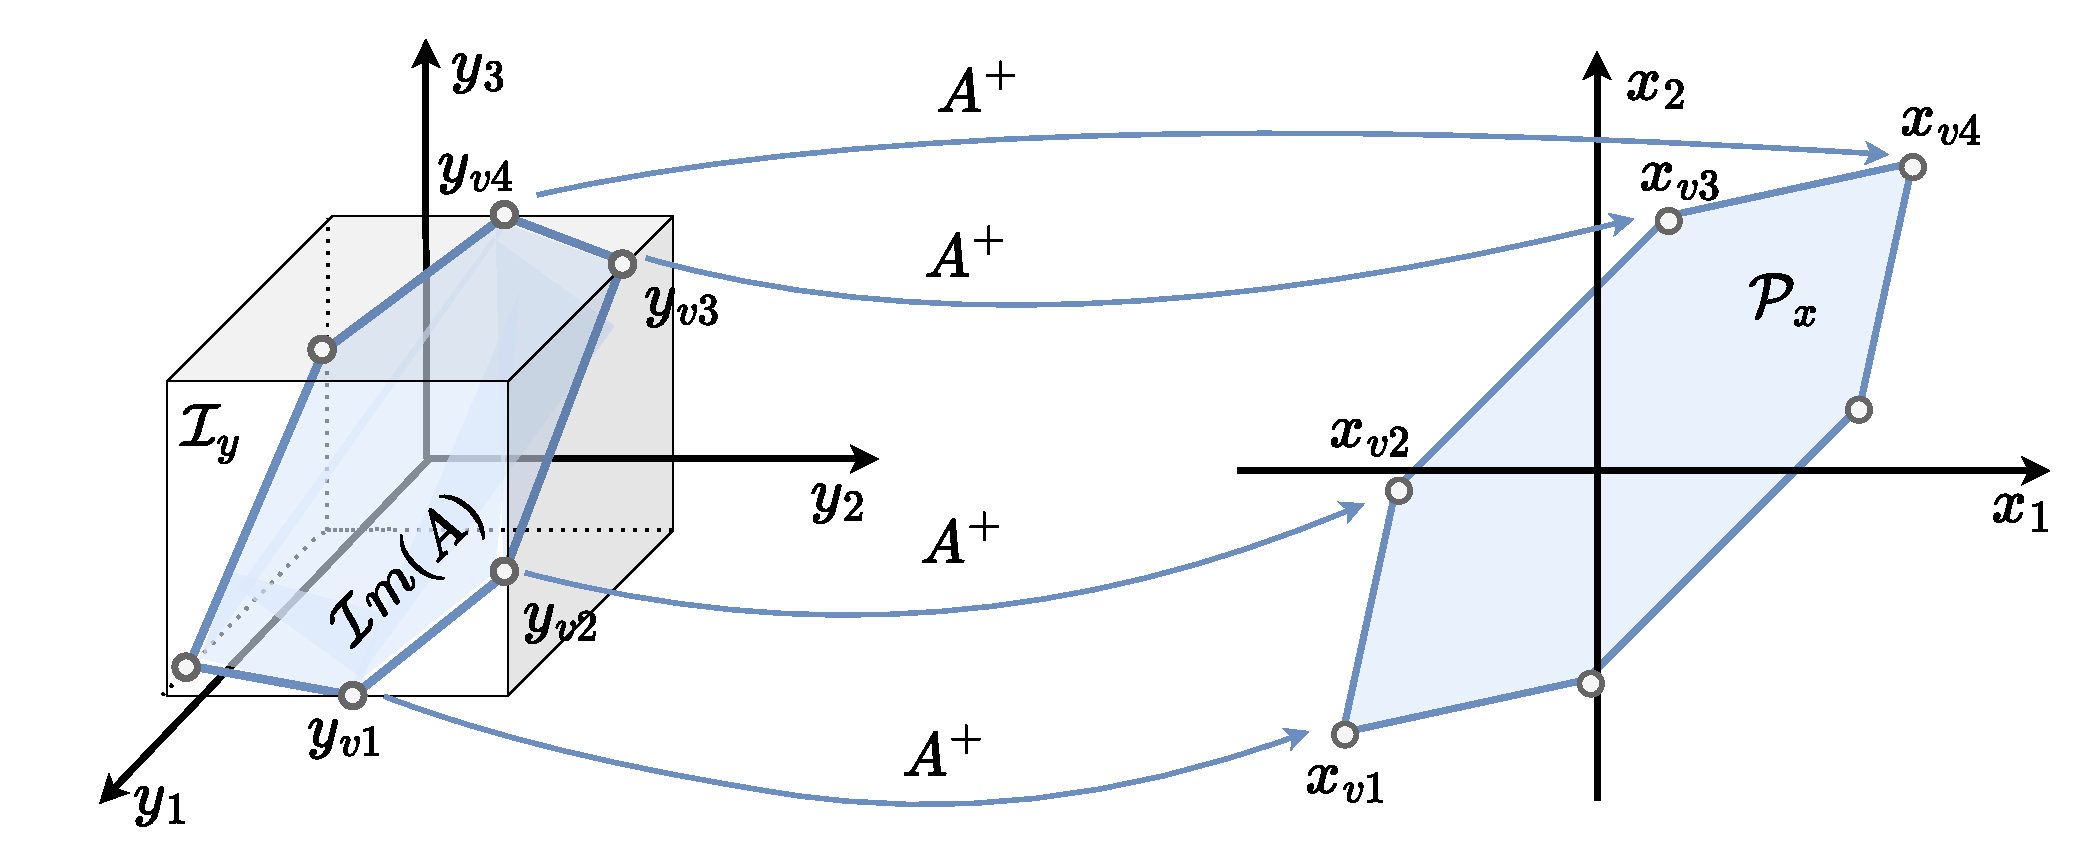
\includegraphics[width=0.8\linewidth]{Papers/images/intersection_algo.pdf}
    \caption{Example intersection polytope $\mathcal{P}_x$ with $n=3$ dimensional interval input set $\mathcal{I}_y$ and $m=2$ dimensional output space. The polytope $\mathcal{P}_x$ vertices $\bm{x}_{vi}$ correspond to the vertices of the intersection $\mathcal{I}_y\cap\img{A}$ denoted as $\bm{y}_{vi}$, through the pseudo-inverse $A^T$ of the matrix $A$.}
    \label{fig:intersection_algo}
\end{figure}

As shown on \Cref{fig:intersection_algo}, the space of all the input vectors $\bm{y}\in\mathbb{R}^n$, bounded within the interval shaped input set $\mathcal{I}_y$, geometrically forms an $n$-dimensional hyperrectangle (orthotope) with $n$ pairs of parallel sides defined by the output limits $\bm{y}\in[\bm{y}_{min},~\bm{y}_{max}]$. The image of the $A$ matrix $\img{A}$ is a $r$-dimensional subspace of the hyperrectangle, where $r$ is the rank of $A$. In  the remainder of this section, the matrix $A$ is, without loss of generality, assumed to be full column rank, i.e. $m$=$r$. 

As discussed in \Cref{ch:inter_formulaiton}, the output space polytope $\mathcal{P}_x$ is the direct affine projection of the intersection between the image $\img{A}$ and the input set $\mathcal{I}_y$ using the pseudo-inverse $A^+$ of the matrix $A$. Therefore this algorithm aims to efficiently find the vertices $\bm{x}_{vi}$ of the polytope $\mathcal{P}_x$, by efficiently finding the vertices $\bm{y}_{vi}$ of the intersection $\mathcal{I}\cap \img{A}$, and project them to the output space using the relationship
\begin{equation}
    \bm{x}_{vi} = A^{+}\bm{y}_{vi}, \qquad \text{where} \quad \bm{y}_{vi}\in\mathcal{I}_y\cap \img{A} \label{eq:compute_vert}
\end{equation}

Therefore the operation of enumerating all the vertices $\bm{x}_{vi}$ of the polytope $\mathcal{P}_x$ can be seen as first finding the $\repr{V}$-representation (the set of vertices $\bm{y}_{vi}$) of the intersection  $\mathcal{I}\cap \img{A}$, followed by its projection to the output space through the pseudo-inverse $A^+$, to obtain the $\repr{V}$-representation of the polytope $\mathcal{P}_x$
\begin{equation}
    \mathcal{P}_x = \conv{A^+\bm{y}_{v1},~A^+\bm{y}_{v1},~\ldots~ }
\end{equation}

\begin{wrapfigure}{r}{0.45\linewidth}
\vspace{-0.5cm}
    \centering
    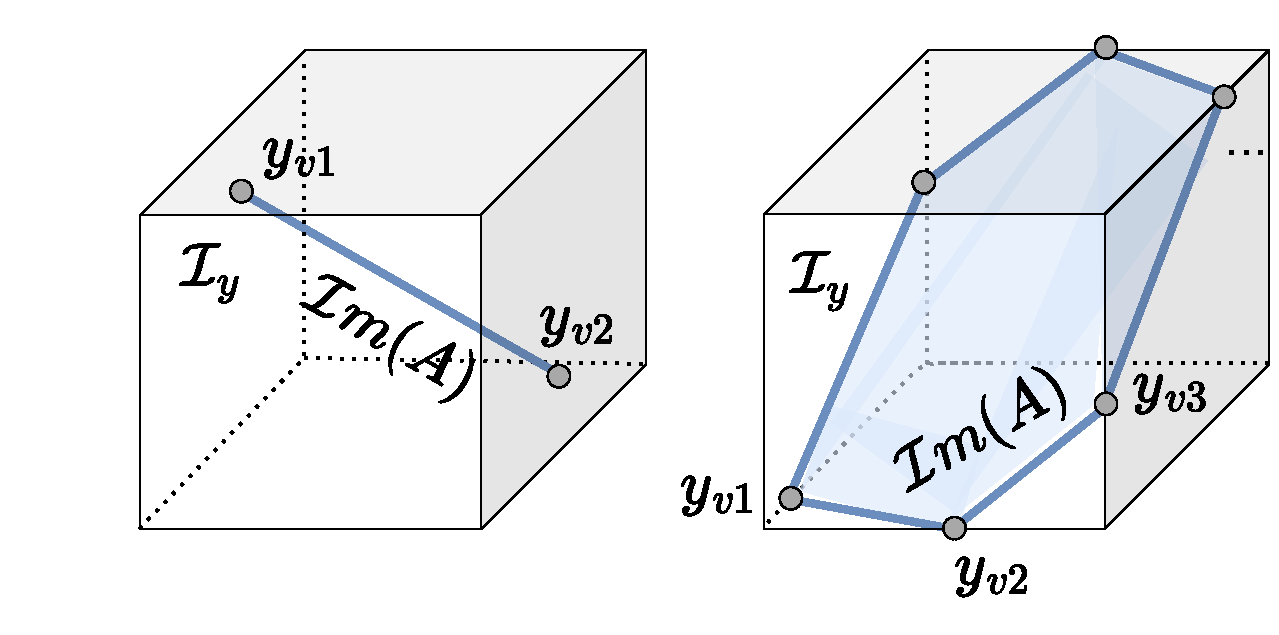
\includegraphics[width=\linewidth]{Papers/images/intersetcion_size.pdf}
    \caption{Example of intersection vertices $\bm{y}_{vi}$ placement on $n\!-\!m$ dimensional faces of hyperrectangle $\mathcal{I}_y$. Left, $m=1$, the vertices $\bm{y}_{vi}$ are on $n\!-\!m\!=\!2$ dimensional faces (sides), while on the right $m=2$ the vertices are on $n\!-\!m\!=\!1$ dimensional faces (edges) }
    \label{fig:size_inter}
\end{wrapfigure}
In their work, \citet{sasaki2011vertex} have shown that, when the input space dimension is $n$ and the image $\img{A}$ dimension is $m$, the extreme values (vertices) of the intersection $\bm{y}_{vi}$ belong to the $n-  m$ dimensional faces of the hyperrectangle $\mathcal{I}_y$. \Cref{fig:size_inter} demonstrates this relationship on an example with the input space dimension $n=3$ and two different output space dimensions $m=1$ and $m=2$. For $m=1$ the vertices $\bm{y}_{vi}$ are on $m-n=2$ dimensional faces of the hyperrectangle corresponding to its sides, and when $m=2$ the vertices  $\bm{y}_{vi}$ are on $m-n=1$ dimensional faces of the hyperrectangle, its edges.

In order to find the  $\repr{V}$-representation of the intersection  $\mathcal{I}\cap \img{A}$, the state-of-the-art algorithms, proposed by \citet{chiacchio_evaluation_1996} and \citet{sasaki2011vertex}, propose an exhaustive search over all the $n$-$m$ dimensional hyperrectangle faces to find the extreme values of $\bm{y}_{vi}$. In this work a new representation of output vector $\bm{y}$ is proposed enabling an efficient navigation of the $n-m$ dimensional hyperrectangle faces. Additionally, an efficient approach to discarding the hyperrectangle faces that cannot contain vertices is integrated in the algorithm, further reducing the complexity of the exhaustive search.

\subsection{Proposed VEPOLI$^2$ algorithm}
Consider an input vector $\bm{y}$ bounded within the input set $\mathcal{I}_y$. It can be defined as
\begin{equation}
    \bm{y} = {\bm{y}}_{min} + \alpha_1 \bm{y}_1+ \alpha_2 \bm{y}_2 + ... + \alpha_n \bm{y}_n
    \label{eq:torque_new}
\end{equation}
where $\alpha_i \in [0,1]$ are scalars weights and vectors $\bm{y}_i$ are orthogonal base vectors in \gls{js}aligned with $i$-th axis of the hyperrectangle $\mathcal{I}_y$, defined as $\bm{y}_i = \begin{bmatrix} 0~\ldots~y_{i,max} - y_{i,min}~\ldots~0 \end{bmatrix}^T$. As shown on the example on \Cref{fig:navigation_y}, the input vector $\bm{y}$ representation (\ref{eq:torque_new}) can be exploited to reach any point within the hyperrectangle $\mathcal{I}_y$, by choosing appropriate scalars $\alpha_i$ in range $[0,1]$. Finding the appropriate values of the scalars $\alpha_i$, for any given $\bm{y}$, can be formulated in a form of linear system
\begin{equation}
\underbrace{\begin{bmatrix}
    \bm{y}_1&\cdots&\bm{y}_n
\end{bmatrix}}_{Y_{n\times n}}\underbrace{\begin{bmatrix}
    \alpha_1\\
    \cdots\\
    \alpha_n
\end{bmatrix}}_{\bm{\alpha}_{n\times 1}} = \bm{y}_{min} - \bm{y}, \qquad  \bm{\alpha} = Y^{-1}(\bm{y}_{min} - \bm{y})
\label{eq:define_Y_Alpha}
\end{equation}
where the matrix $Y$, containing the orthogonal base vectors $\bm{y}_i$, is square and always invertible. 
Furthermore, as the intersection vertices $\bm{y}_{vi}$ belong to the $n$-$m$ dimensional faces of the input hyperrectangle $\mathcal{I}_y$, the representation (\ref{eq:torque_new}) can be further simplified. Any input vector $\bm{y}$, belonging to an $n-m$ dimensional face of the hyperrectangle $\mathcal{I}_y$, can be reached by choosing the appropriate values of $n-m$ scalars $\alpha_i\in[0,1]$, while the other $m$ scalars are fixed to either 0 or 1 ($\alpha_i\in\{0,1\}$).

\begin{figure}
    \centering
    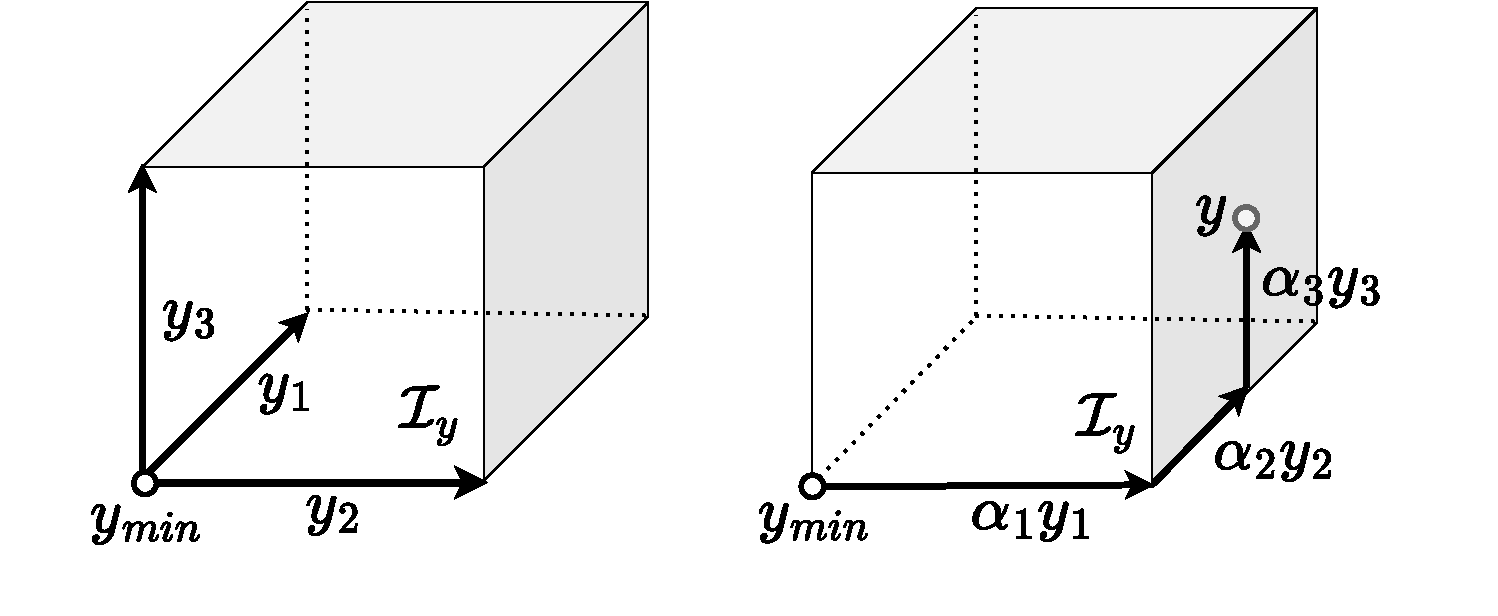
\includegraphics[width=0.6\linewidth]{Papers/images/navigation_y.pdf}
    \caption{Example of the vector representation (\ref{eq:torque_new}) on the $n\!=\!3$ dimensional hyperrectangle $\mathcal{I}_y$. Base vectors $\bm{y}_i$ are shown on the left, and on the right their linear combination using scalars $\alpha_i$ is shown reaching the point $\bm{y}\in\mathcal{I}_y$.}
    \label{fig:navigation_y}
\end{figure}
Furthermore, $n-m$ scalars $\alpha_i\in[0,1]$ can be interpreted as coordinates of the $n-m$ dimensional face, while the remaining $m$ fixed scalars $\alpha_i\in\{0,1\}$, to either 0 or 1, define its origin $\bm{y}_o$
\begin{equation}
    \bm{y}_o = \bm{y}_{min} + \alpha_1 \bm{y}_1+ ... + \alpha_m \bm{y}_m, \qquad \alpha_i \in\{0,1\}
\end{equation} 
Then any $\bm{y}$, belonging to a face of the hyperrectangle, can be expressed using the face's origin $\bm{y}_o$ and its set of $n-m$ scalars $\alpha_i$ 
\begin{equation}
    \bm{y} = \bm{y}_o ~+ ~\alpha_{m+1}\bm{y}_{m+1} +~\cdots~ +\alpha_{n}\bm{y}_{n}, \qquad \alpha_i \in [0,1]
\end{equation}
The vector $\bm{\alpha}\in\mathbb{R}^n$ can be conveniently divided into two components, $\bm{\alpha}_o\in\mathbb{R}^m$ containing $m$ scalars $\alpha_i$ defining the origin of the face and $\bm{\alpha}_x\in\mathbb{R}^{n-m}$ containing $n-m$ scalar coordinates $\alpha_i$ of the face. Additionally, the same can be done with the matrix $Y$, divided in $Y_o\in\mathbb{R}^{n\times m}$ corresponding to $m$ base vectors used to define the origin $\bm{y}_o$, and $Y_x\in\mathbb{R}^{n\times (n-m)}$
 corresponding to the $n\!-\!m$ base vectors $\bm{y}_i$ spanning the face. Then the origin $\bm{y}_o$ and the final vector $\bm{y}$ can be expressed as
 \begin{equation}
    \bm{y}_o = \bm{y}_{min} + Y_o\bm{\alpha}_{o}, \qquad \bm{y} = \bm{y}_o +  Y_x\bm{\alpha}_{x}, \qquad \bm{\alpha}_{o}\in\{\bm{0},\bm{1}\},~~ \bm{\alpha}_{x}\in[\bm{0},\bm{1}]
    \label{eq:matrix_new_y}
\end{equation}
Therefore, in order to find all the vertices $\bm{y}_{vi}$ of the intersection $\mathcal{I}_y\cap\img{A}$, the proposed VEPOLI$^2$ algorithm tests if there exists a point intersection (a vertex) between the $\img{A}$ and every single one of the $n-m$ dimensional faces of the hyperrectangle $\mathcal{I}_y$.

Since all the $\bm{y}$ belonging to the image $\img{A}$ can be expressed as $\bm{y}=A\bm{x}$, this relationship can be further exploited to relate the vertices $\bm{y}_{vi}$ of the intersection $\img{A}\cap\mathcal{I}_y$ and the vertices $\bm{x}_{vi}$ of the final polytope $\mathcal{P}_x$. For each face to be tested, the equations  (\ref{eq:inter_hyp_revisit_algo}) and (\ref{eq:compute_vert}) can be combined
\begin{equation}
    \bm{y}_{vi} = A \bm{x}_{vi} = \bm{y}_{oi} + \alpha_{m+1} \bm{y}_{m+1}+ ~...~ + \alpha_n \bm{y}_n \label{eq:step2}
\end{equation}
where, $\bm{y}_{oi}$ is the origin of the $n\!-\!m$ dimensional face, spanned by the scalar $n\!-\!m$ scalars $\bm{\alpha}_{xi}$. For each face $i$, by fixing the appropriate $m$ scalars $\bm{\alpha}_{oi}$ to 0 or 1, its origin $\bm{y}_{oi}$ can be calculated using (\ref{eq:matrix_new_y}). In order to determine if this face contains the vertex of the intersection $\mathcal{I}_y\cap\img{A}$, a linear system derived from equation~(\ref{eq:step2}) can be solved. This system finds the remaining $n\!-\!m$ scalars $\bm{\alpha}_{xi}$ as well as the corresponding vertex $\bm{x}_{vi}$ at the same time
\begin{equation}
    \underbrace{\begin{bmatrix}A&-\bm{y}_{m+1} \, \dots \, -\bm{y}_{n} \end{bmatrix}}_{Z_{n\times n}} \begin{bmatrix}\bm{x}_{vi}\\ \alpha_{m+1} \\ \vdots\\\alpha_{n} \end{bmatrix} =\begin{bmatrix}A &Y_{xi} \end{bmatrix}\begin{bmatrix}\bm{x}_{vi}\\ \bm{\alpha}_{xi} \end{bmatrix}  = \bm{y}_{oi}, \qquad \begin{bmatrix}\bm{x}_{vi}\\ \bm{\alpha}_{xi} \end{bmatrix} = Z^{-1}\bm{y}_{oi}, 
    \label{eq:linear_system_full}
\end{equation}
Matrix $Z\in\mathbb{R}^{n\times n}$ is a square matrix where each one of the vectors $\bm{y}_i$ is independent. If the matrix $Z$ is singular, geometrically, the image $\img{A}$ is parallel to the face being tested, therefore no intersections exist. If $Z$ is invertible and the $n-m$ scalars $\bm{\alpha}_{xi}$ are obtained, a simple check if $\bm{\alpha}_{xi} \in [\bm{0},\bm{1}]$ can be used to determine if $\bm{x}_{vi}$ is a vertex of the polytope $\mathcal{P}_x$. Geometrically, the condition $\bm{\alpha}_{xi} \in [\bm{0},\bm{1}]$ ensures that the intersection point between the $\img{A}$ and the $n\!-\!m$ dimensional face, is also inside $\mathcal{I}_y$. One of the nice features of this approach is that it does not require an explicit inversion of $A$, as in equation~(\ref{eq:compute_vert}), to obtain the set of vertices composing $\mathcal{P}_x$.

Following three sections bring the approaches further improving the efficiency of the proposed algorithm. First, the dimension of the matrix $Z$ is reduced using the \gls{svd}, then the parallelism of the faces of the hyperrectangle is exported to reduce the number of the computations of the system (\ref{eq:linear_system_full}). Finally, an additional condition is introduced enabling to discard faces and avoid the unnecessary matrix inversions.


\subsubsection{Matrix size reduction using the SVD}

In order to reduce the dimension of the linear system (\ref{eq:linear_system_full}), the \gls{svd} \cite{klema_singular_1980} of $A^T$ is used
\begin{equation}
     A^T =  U  \underbrace{\begin{bmatrix}S & O_{m\times (n-m)}\end{bmatrix}}_{\Sigma}\underbrace{\begin{bmatrix}V_1^T \\ V_2^T \end{bmatrix}}_{V^T}
\end{equation}
where $S= diag( \sigma_1 \dots \sigma_m)$ is a diagonal matrix containing the $m$ singular values of $A^T$. $V_1^T \in \mathbb{R}^{m \times n}$ is the projector from the input space onto the image of $\img{A}$ and $V_2^T \in \mathbb{R}^{n-m \times n}$ is a basis of $\ker{A}$. $V_1^T$ and $V_2^T$ are orthogonal vector subspaces yielding $V_2^T V_1 = 0$ and thus 
\begin{equation}
    V_2^T A\bm{x} = \bm{0}
\end{equation}
Then, multiplying the equation (\ref{eq:linear_system_full}) with $V^T_2$
\begin{equation}
    V_2^T\begin{bmatrix}A &Y_{xi} \end{bmatrix}\begin{bmatrix}\bm{x}_{vi}\\ \bm{\alpha}_{xi} \end{bmatrix}  = \underbrace{V_2^TA\bm{x}_{vi}}_{\bm{0}} + V_2^TY_{xi}\bm{\alpha}_{xi} = V_2^T\bm{y}_{oi} 
\end{equation}
allows to reduce the system (\ref{eq:linear_system_full}) to
\begin{equation}
    \underbrace{V_2^T\begin{bmatrix}-\bm{y}_{m+1} ~\dots~ -\bm{y}_{n} \end{bmatrix}}_{T_{(n-m)\times (n-m)}} \bm{\alpha}_x  = V_2^TY_{xi}\bm{\alpha}_{xi} = V_2^T\bm{y}_{oi}
    \label{eq:linear_system_svd}
\end{equation}
If $T$ is invertible, $\bm{\alpha}_{xi}$ can be computed by
\begin{equation}
\bm{\alpha}_{xi} = T^{-1}V_2^T\bm{y}_{oi}
\label{eq:svd_linear_sys_step1}
\end{equation}
When the computed $\bm{\alpha}_{xi}$ complies with the check $\bm{\alpha}_{xi} \in [\bm{0},\bm{1}]$,  the corresponding polytope vertex can be calculated as
\begin{equation}
    \bm{x}_{vi} = A^{+} \big( \bm{y}_{oi} + Y_{xi}\bm{\alpha}_{xi}\big)
\label{eq:svd_linear_sys_step2}
\end{equation}

This new approach requires the calculation of the \gls{svd} and the pseudo-inverse $A^{+}$. Nevertheless, since the pseudo-inverse can be efficiently calculated from the \gls{svd} as $A^{+} = U\Sigma^{T+}V^T$ and since both the \gls{svd} and pseudo-inverse are calculated once per algorithm run, the computation efficiency is greatly improved due to the matrix dimension reduction from $n$ to $(n-m)$ when inverting $T$ instead of $Z$.

\begin{figure}[!t]
    \centering
    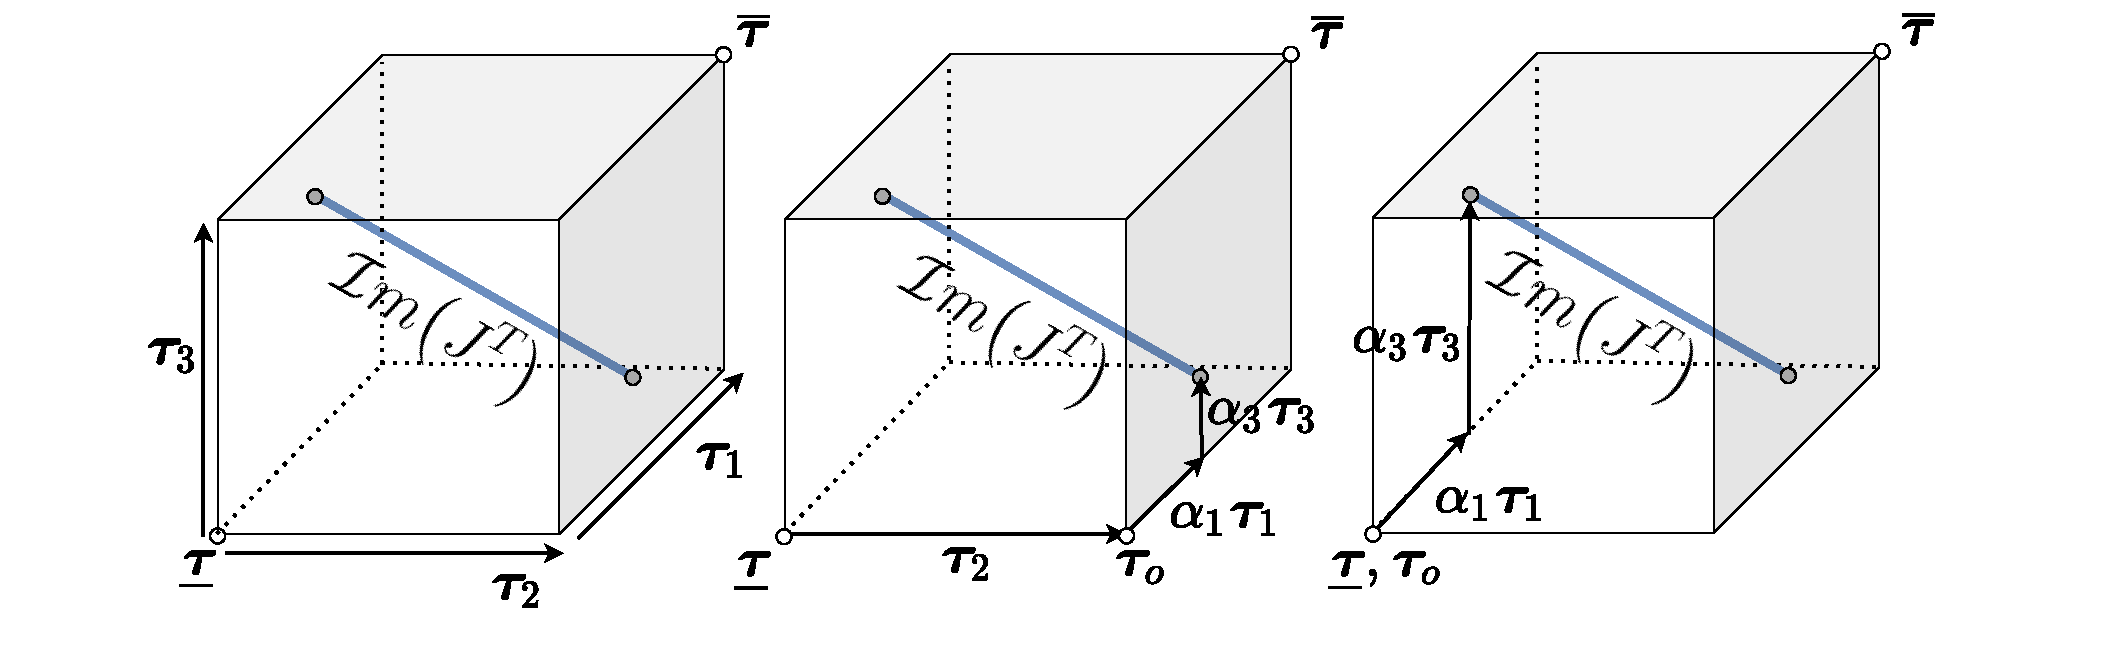
\includegraphics[width=0.9\linewidth]{Papers/images/intersection_example.pdf}
    \caption{Example of input space interpretation of the VEPOLI$^2$ algorithm for the system $n$=$3$ and $m$=$1$. The two vertices of the intersection $\{\bm{y}_{v1},\bm{y}_{v2}\}$ are reached by solving the linear system (\ref{eq:linear_system_full}) or (\ref{eq:linear_system_svd}). The vertices belong to the parallel ($n\!-\!m\!=\!2$ dimensional faces) sides of the hyperrectangle $\mathcal{I}_y$.  }
    \label{fig:intersection_example}
\end{figure}

\begin{wrapfigure}[12]{r}{0.25\linewidth}
\vspace{-0.5cm}
    \centering
    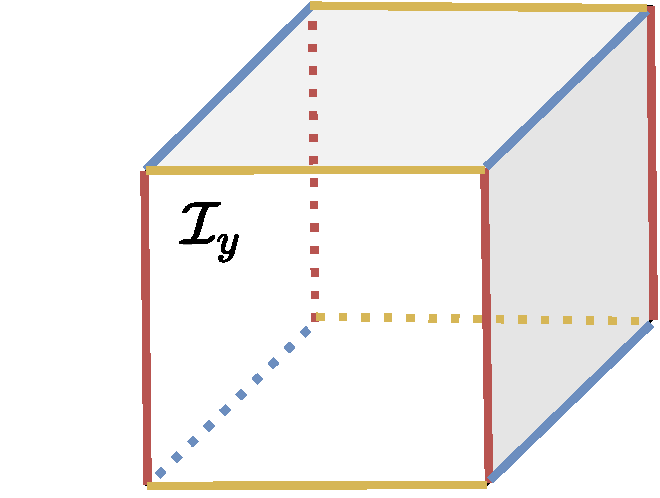
\includegraphics[trim=1.5cm 0 0 0,clip=true,width=\linewidth]{Papers/images/parallel.pdf}
    \caption{All the parallel edges of the 3D hyperrectangle shown in differing colours. It has 3 (red, blue, yellow) sets of 4 parallel edges, 12 edges in total.}
    \label{fig:parallel}
\end{wrapfigure}
\subsubsection{Exploiting the parallelism of the hyperrectangle faces} 
The number of $n-m$ dimensional faces of an $n$ dimensional hyperrectangle $\mathcal{I}_y$ can be calculated using the expression
$$
N_{n,(n-m)}= 2^{n-(n-m)}\binom{n}{n-m} =  2^{m}\binom{n}{m} 
$$
More precisely, an $n$ dimensional hyperrectangle has $\big(\begin{smallmatrix}n\\m\end{smallmatrix}\big)$ sets of $2^m$ parallel faces with the dimension $n\!-\!m$. 
As illustrated on \Cref{fig:parallel}, a 3D ($n\!=\!3$) hyperrectangle has $\big(\begin{smallmatrix}3\\1\end{smallmatrix}\big)\!=\!3$ sets of $2^{2}\!=\!4$ parallel ($n\!-\!m\!=\!1$) edges, as well as $\big(\begin{smallmatrix}3\\2\end{smallmatrix}\big)=3$ sets of $2^1\!=\!2$ parallel ($n\!-\!m\!=\!2$) sides. 

All the parallel $n\!-\!m$ dimensional faces of the hyperrectangle $\mathcal{I}_y$ can be spanned using the same set of $n\!-\!m$ scalars $\bm{\alpha}_{xi}$, while the remaining $m$ scalars $\bm{\alpha}_{oi}$ can be used to find their $2^m$ origins $\bm{y}_{oi}$.

\Cref{fig:intersection_example} illustrates the case where $\img{A}$ is a line ($m=1$) and the input space is $n=3$ dimensional. In this case the intersection vertices $\{\bm{y}_{v1},\bm{y}_{v2}\}$ lie in $n$-$m$=$2$ dimensional hyperrectangle faces. In that example, both vertices $\bm{y}_{vi}$ are placed on two parallel faces, spanned by the two scalars $\alpha_1$ and $\alpha_3$, while the scalar $\alpha_2$, set to $0$ or $1$, is used to find their origins $\bm{y}_{oi}$.

In the linear system (\ref{eq:linear_system_svd}), matrix $T$ has the same content for each parallel face of the hyperrectangle. Therefore, the inverse $T^{-1}$ can be recalculated only once per set of parallel faces. Then, for each of the $2^m$ parallel faces within the set, the vertex $\bm{x}_{vi}$ and the corresponding $\bm{\alpha}_{xi}$, can be obtained by multiplying the $2^n$ origins $\bm{y}_{oi}$ with $T^{-1}$, as described by (\ref{eq:svd_linear_sys_step1}-\ref{eq:svd_linear_sys_step2}).

Overall, in order to test all possible combinations of the $n\!-\!m$ dimensional faces which may contain vertices of the intersection (and in term the final polytope $\mathcal{P}_x$), the total of $\big(\begin{smallmatrix}n\\m\end{smallmatrix}\big)$=$\frac{n!}{m!(n-m)!}$ inversions of the matrix $T$ and  $2^m\big(\begin{smallmatrix}n\\m\end{smallmatrix}\big)$ checks $\bm{\alpha}_{xi} \in [\bm{0},\bm{1}]$ have to be performed.

In the case depicted in \Cref{fig:intersection_example} ($n$=$3$, $m$=$1$), $T$ is inverted only $\big(\begin{smallmatrix}3\\1\end{smallmatrix}\big)$=$3$ times and conditions are evaluated 6 times, which corresponds exactly to the number of sides of the hyperrectangle. In the same example, if the output space would be 2D ($n$=$3$, $m$=$2$) the number of $T$ inversions is 3 and the number of condition evaluation is 12, which corresponds to the number of edges of the hyperrectangle. 

\subsubsection{Matrix inverse condition} 

The most time consuming aspect of the proposed VEPOLI$^2$ algorithm is the relatively high number of matrix $T$ inversions. Therefore this section proposes a necessary condition to discard the sets of faces that cannot contain a vertex and avoid unnecessary matrix $T$ inversions.

\begin{wrapfigure}{r}{0.35\linewidth}
    \centering
    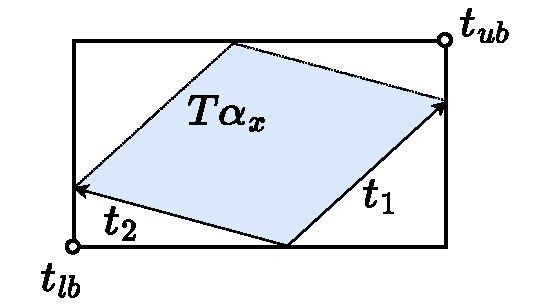
\includegraphics[width=\linewidth]{Papers/images/matrix_condition.pdf}
    \caption{The bounding-box calculated using the equation (\ref{eq:bounds_condition}). The size of the example system is $n\!-\!m\!=\!2$, where $\bm{t}_1,\bm{t}_2$ are column vectors of the matrix $T$.}
    \label{fig:matrix_condition}
\end{wrapfigure}
Due to the constrained nature of the scalars $\bm{\alpha}_{xi}\in[\bm{0},\bm{1}]$, it is possible to efficiently calculate the bounds (${\bm{t}_{ub}}$ and $\bm{t}_{lb}$) on the $T\bm{\alpha}_{xi}$ 
\begin{equation}
    T\bm{\alpha}_{xi}  \in [\bm{t}_{lb}, \bm{t}_{ub}]\label{eq:necesassry_condition1}
\end{equation}
As the column vectors $\bm{t}_i$ within the matrix $T$ are, in the general case not orthogonal, the min-max interval shaped set can not exactly characterise the feasible set of $T\bm{\alpha}_{xi}$. However, an interval that over-approximates it, can be found very efficiently by row-wise summing only positive and only negative elements $t_{ij}$ of  $T$
\begin{equation}
t_{i,lb} = \sum_j \max(t_{ij}, 0), \qquad
t_{i,lb} = \sum_j \min(t_{ij}, 0) 
\label{eq:bounds_condition}
\end{equation}
As shown on \Cref{fig:matrix_condition}, this creates a bounding box around the space defined by  $T\bm{\alpha}_{xi}$.

In order for the system (\ref{eq:linear_system_svd}) to have a solution, the null-space projections of the vectors $\bm{y}_{oi}$ have to respect the same bounds as well
\begin{equation}
    V_2^T\bm{y}_{oi} \in [\bm{t}_{lb}, \bm{t}_{ub}]\label{eq:necesassry_condition}
\end{equation}
Therefore, using this bounding box, the necessary check can be devised for the inversion of the matrix $T$. If all the $2^m$ combinations of $V_2^T\bm{y}_{oi} \notin [\bm{t}_{lb}, \bm{t}_{ub}] $, the system (\ref{eq:linear_system_svd}) cannot have a solution which satisfies $\bm{\alpha}_{xi} \in [\bm{0},\bm{1}]$, and there is no need to invert $T$ to figure it out.

The condition $V_2^T\bm{y}_{oi} \in [\bm{t}_{lb}, \bm{t}_{ub}] $ is a necessary condition, however as the interval $[\bm{t}_{lb}, \bm{t}_{ub}]$ presents an over-approximation of the achievable set $T\bm{\alpha}_x, \bm{\alpha}_x\in[\bm{0}, \bm{1}]$, it is not a sufficient condidion. 

The bounding box (\ref{eq:bounds_condition}), as well as the $2^m$ face origins $\bm{y}_{oi}$ can be calculated efficiently, allowing for a computationally inexpensive reduction in the number of matrix inversions. The upper bound on the number of matrix inversions $N_{inv}$ can be found by studying the worst-case scenario, where all the origins $\bm{y}_{oi}$ pass the condition (\ref{eq:necesassry_condition}). In this case the number of inversion corresponds to the binomial $\binom{n}{m}$. In the general case, the number of matrix inversions $N_i$ is bounded and equals to  
$$N_{inv}\leq\binom{n}{m}=\frac{n!}{m!(n-m)!}$$
The number of checks $N_c$ of the condition $\bm{\alpha}_{xi} \in [\bm{0},\bm{1}]$, per matrix inversion, is bounded as well, as the origin vectors $\bm{y}_{oi}$ that do not comply with the necessary condition (\ref{eq:necesassry_condition}) can be discarded from the these checks as well
$$
N_c\leq2^m
$$

\subsection{Performance and complexity comparison}\label{sec:complexity}
To demonstrate the efficiency of the VEPOLI$^2$ algorithm, it is compared against the polytope vertex search algorithm introduced by \citet{chiacchio_evaluation_1996}. Furthermore the comparison is extended to the algorithm proposed by \citet{sasaki2011vertex} which is, to our knowledge, the only algorithm exploiting the geometric structure of the intersection formulation polytope with interval limits (\ref{eq:inter_hyp_revisit_algo}).

\begin{table}[!h]
    \centering
    \begin{tabular}{|c|c|c|c|}
       \hline
      \textbf{ System size }& \textbf{Chiacchio}\cite{chiacchio_evaluation_1996} & \textbf{Sasaki} \cite{sasaki2011vertex}  &  \textbf{VEPOLI$^2$} \\
       \hline
       $(n,m)$& matrix inversions: $ \frac{2n!}{m!(2n-m)!}$  & $ \frac{n!}{m!(n-m)!} $ & $ \leq \frac{n!}{m!(n-m)!}$ \\
       &  matrix size:  $ 2n \times 2n$ & $m\times m$  & $n$-$m$ $\times$ $n$-$m$\\
       & time[ms]: mean $\pm$ std (max) & & \\
       \hline
       $(4,2)$ &  24 & 6 & 4.2$\pm$1.4 (6) \\ 
       & 8$\times$8 & 2$\times$2 & 2$\times$2 \\ 
       & 2.7$\pm$0.1 (3.6) & 0.93$\pm$0.1 (1.1) & 0.64$\pm$0.1 (1.5) \\ 
       \hline
       $(4,3)$ &  32 & 4 & 2.9$\pm$1.1 (4) \\ 
       & 8$\times$8 & 3$\times$3 & 1$\times$1 \\ 
       & 3.7$\pm$0.3 (6.0) & 0.79$\pm$0.08 (1.4) & 0.54$\pm$0.1 (1.4) \\ 
       \hline
       $(6,3)$ & 220 & 20 & 2.8$\pm$2.5 (10) \\ 
        & 12$\times$12 & 3$\times$3 & 3$\times$3 \\ 
       & 14.2$\pm$0.9 (20) & 2.1$\pm$0.2 (3.4) & 1.5$\pm$0.2 (2.7) \\ 
       \hline
      $(6,6)$&   64 & 1 & 1$\pm$0 (1)\\
        &  12$\times$12 & 6$\times$6 & 6$\times6$\\
       & 34.7$\pm$1 (44.3) & 0.32$\pm$0.07 (0.56) & 0.24$\pm$0.04 (0.46)\\
       \hline
      $(7,3)$&    364 & 35 & 7.3$\pm$4.2 (20)\\
        & 14$\times$14 & 3$\times$3 & 4$\times4$\\
       & 25$\pm$0.5 (27) & 3.5$\pm$0.1 (5.4) & 2.6$\pm$0.2 (4.3)\\
       \hline
      $(7,6)$& 448 & 7 & 6.4$\pm$1 (7)\\
        & 14$\times$14 & 6$\times$6 & 1$\times$1\\
       & 150$\pm$34 (360) & 1.6$\pm$0.5 (4) & 1.2$\pm$0.3 (3.0)\\
       \hline
    \end{tabular}
    \caption{Complexity and execution time (in milliseconds) comparison for three different vertex search algorithms. The comparison provided for the number of matrix inversions, matrix size and time of execution, averaged over 1000 random systems. }
    \label{tab:complexity_results}
\end{table}

The three algorithms have been tested on finding the $\repr{V}$-representation of the three different systems, inspired by the wrench ($\bm{f}\in\mathbb{R}^m$) polytope $\mathcal{P}_f$ enumeration for three different robots: a 4R planar robot ($n$=$4$), the {Universal Robots} UR5 6DoF robot ($n$=$6$) and the {Franka Emika Panda} 7DOF robot ($n$=$7$). The planar 4R robot is used to calculate its planar force ($m=2$) and its planar wrench ($m=3$) polytope, while UR5 and Panda are used to calculate \gls{cs} force ($m=3$) and wrench ($m=6$) polytopes. The results are averaged over 1000 randomly generated matrices $A$ and input sets $\mathcal{I}_y$. All algorithms have been implemented in the programming language Matlab and tested on a laptop equipped with a 1.90GHz Intel i7-8650U processor. The source code of the experiment is publicly available on GitLab\footnote{Gitlab: \url{https://gitlab.inria.fr/auctus-team/people/antunskuric/papers/polytope_vertex_search}}.

\Cref{tab:complexity_results} shows the results of this complexity evaluation. The VEPOLI$^2$ algorithm substantially reduces the number of matrix inversions and thus reduces the processing time considerably: $4$-$10\times$ faster execution than Chiacchio's algorithm and on average 30\% faster than Sasaki's. Results show that, even for the generic cases that correspond to the 6DOF ($n=6$) and 7DOF ($n=7$) industrial robots, the VEPOLI$^2$ algorithm is capable of evaluating both force ($m=3$) and wrench ($m=6$) polytope vertices under $3ms$. Such a low processing time opens numerous opportunities for the online use of polytope based capacity, evaluation especially in the area of robot control. 

\Cref{fig:panda_ur5_force} shows the visualisation of the \gls{cs} force ($m=3$) polytope for the UR5 and Panda robots. Both polytopes are calculated using the VEPOLI$^2$ algorithm.

\begin{figure}
    \centering
    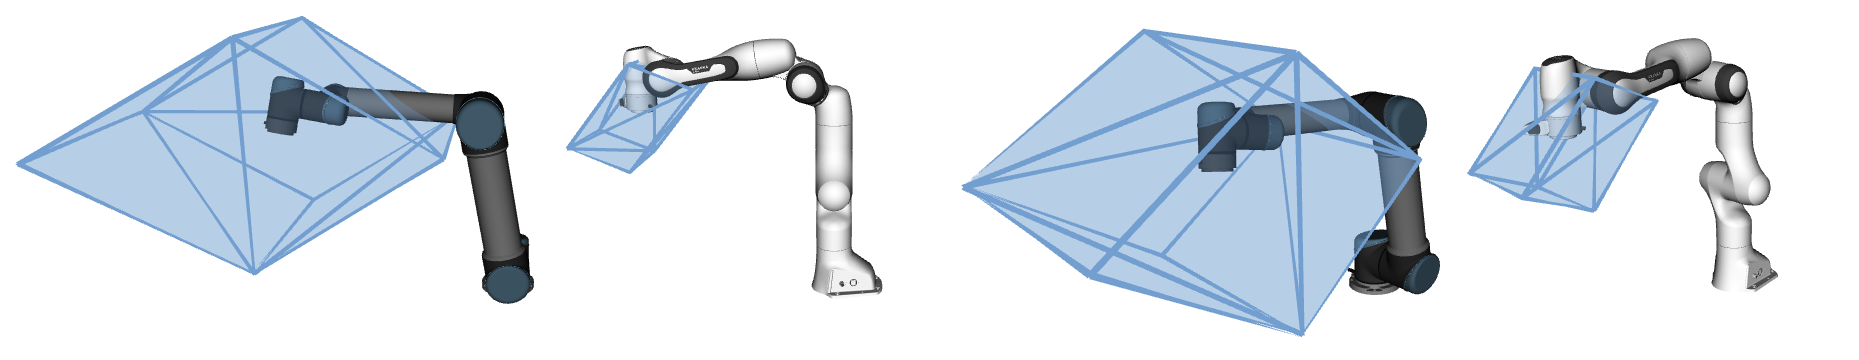
\includegraphics[width=\linewidth]{Papers/images/panda_ur5.png}
    \caption{Two different views of Panda ($n=7$) and UR5 ($n=6$) robot's force polytope ($m=3$) calculated using the VEPOLI$^2$ algorithm. Both robots and polytopes are shown in the same scale (1m : 1000N). The figure shows that the UR5 has much larger polytope than Panda robot. This is due to its larger force capacity, as UR5 is rated for 5kg loads whereas Panda is rated for 3kg loads.}
    \label{fig:panda_ur5_force}
\end{figure}

\subsection{Discussion on limitations}
This algorithm, being based on the algorithm proposed by \citet{sasaki2011vertex}, is still based on the exhaustive search. Even though significantly reducing the complexity of the Sasaki's method, it is not particularly well suited for high dimensions $n$ of the input space, especially if the difference between the input and the output space dimension $n\!-\!m$ is large. 

The algorithm has two computational bottlenecks: the number of matrix $T$ inversions $N_{inv}$ and the number of checks $\bm{\alpha}_{xi} \in [\bm{0},\bm{1}]$ per matrix inversion $N_c$.

If the system has high dimensional input space and low dimensional output space ($n\gg m$) then the number of matrix inversions $N_{inv}=\binom{n}{m}$ will be large, while the number of checks $N_c=2^m$  will be low. 
On the other hand, if the system has both high dimensional input space and high dimensional output space ($n\approx m$ and $n,m\gg0$), then the number of matrix inversions $N_{inv}=\binom{n}{m}$ will be relatively low and will not be the limiting factor, but the number of checks $N_c=2^m$ which will be very high. Therefore, although the algorithm is created in a generic form and can find the $\repr{V}$-representation of any polytope belonging to this family, it is particularly efficient when the dimensions of the input and the output space are relatively low. 

Furthermore, as the VEPOLI$^2$ algorithm exploits the null-space $\ker{A}$ of the matrix $A$ to gain on efficiency, it is not suitable for the systems where the matrix $A$ is square ($m\!=\!n$), as in that case the null-space does not exist $\ker{A}=\{\varnothing\}$. However, as discussed in the \Cref{par:equivalent_proj}, this specific case of interval projection is much easier to work with as it corresponds to the projection formulation, which $\repr{V}$-representation can be determined in a straight-forward manner, as described in \Cref{ch:proj_algos_v}, by projecting the vertices of the hyperrectangle to the output space.


\begin{algorithm}[!t]
\caption{The VEPOLI$^2$ algorithm pseudo-code}
\begin{algorithmic}
\REQUIRE $A$, $\bm{y}_{min}$, $\bm{y}_{max}$ (Eq. \ref{eq:interval_revisit_algo}) 
\STATE $U, \Sigma, V^T \leftarrow svd(A^T)$ 
\STATE $A^{+} = U\Sigma^{T+}V^T$
\STATE $V_1,\, V_2  \leftarrow V $
\STATE calculate $n$ base vectors $\bm{y}_1 \dotsc \bm{y}_n$ (Eq. \ref{eq:torque_new})

\STATE init $\repr{V}$-rep: $X_v$, $Y_v$ $\!\leftarrow\! []$

\FORALL{  $\big(\begin{smallmatrix}n\\m\end{smallmatrix}\big)$ combinations of $m$ fixed $\alpha_i$ } 
\STATE construct matrices $Y_o$ and $Y_x$
\STATE $T = V_2^TY_x$
\IF{matrix T invertible}
\STATE find bounds $\bm{t}_{lb},\bm{t}_{ub}$ (Eq. \ref{eq:bounds_condition})
\STATE init list of origins $\bm{y}_o$ satisfying the condition (Eq. \ref{eq:necesassry_condition}): $L_o$ $\!\leftarrow\! []$ 
\FORALL{   $2^m$ vectors $\bm{\alpha}_o$ }
\STATE $\bm{y}_o = \bm{y}_{min} +  Y_o\bm{\alpha}_o$ 
\IF{$ V_2^T\bm{y}_o \in [\bm{t}_{lb},\bm{t}_{ub}] $}
\STATE update candidates: $L_o \!\leftarrow\! [L_o,~ \bm{y}_o]$
\ENDIF
\ENDFOR

\IF{$L_o$ not empty}
\STATE calculate the inverse $T^{-1}$
\FORALL{   $\bm{y}_o$ in $L_o$ }
\STATE $\bm{\alpha}_x = T^{-1}V_2^T\bm{y}_o $
\IF{$ \bm{\alpha}_x \in [\bm{0},\bm{1}] $}
\STATE $\bm{y}_{v} = \bm{y}_o + Y_x\bm{\alpha}_x$ 
\STATE $\bm{x}_{v} = A^{+}\bm{y}_{v}$ 
\STATE update $\repr{V}$-rep: ${X}_{v} \!\leftarrow\! [{X}_{v},~ \bm{x}_v ]$, ${Y}_{v} \!\leftarrow\! [{Y}_{v},~ \bm{y}_v ]$ 
\ENDIF
\ENDFOR
\ENDIF


\ENDIF

\ENDFOR
\RETURN $\repr{V}$-rep: $X_v$, $Y_v$

\end{algorithmic}
\label{alg:algo_1}
\end{algorithm}

\subsection{Algorithm implementation}
\qrimg{qrcodes/pycapacity.png}{https://auctus-team.github.io/pycapacity/}{\codet{pycapacity}}
The pseudo-code of the proposed algorithm is given in \Cref{alg:algo_1}, while an efficient open-source Python implementation is publicly available within the package \codet{pycapacity}\footnote{\href{https://auctus-team.github.io/pycapacity/}{https://auctus-team.github.io/pycapacity/}}, which is described more in detail in \Cref{ch:software}.\\\\
\Cref{ch:robot_robot_carrying} brings the application of the VEPOLI$^2$ algorithm for the real-time robot control in the human-robot collaboration scenario, where the algorithm is exploited in order to calculate the robot's wrench capacity polytope online. 



\section{ICHM: New algorithm for polytope approximation}
\label{ch:algorihtm_ichm}

This section introduces a new polytope approximation algorithm called \textbf{I}mplicit (or \textbf{I}terative) \textbf{C}onvex-\textbf{H}ull \textbf{M}ethod (ICHM). This algorithm is based \gls{chm}, developed by \citet{lassez1992quantifier}, and tailored specifically for the generic (implicit) polytope formulation 
\begin{equation}
    \mathcal{P}_x = \big\{ \bm{x}\in \mathbb{R}^{m}\, |\,A\bm{x} = B\bm{y} + \bm{b}, \quad  \bm{y}\in\mathcal{P}_y  \big\}
    \label{eq:generic_polyt_view_revisit2}
\end{equation}
where the input set $\mathcal{P}_y$ can be expressed with its $\repr{H}$-representation
\begin{equation}
    \mathcal{P}_y = \big\{ \bm{y}\in \mathbb{R}^{n}\, |\,H_y\bm{y} \leq \bm{d_y}\big\}
    \label{eq:generic_poly_input_set_revisit2}
\end{equation} 
This polytope formulation, as discussed in \Cref{ch:collab_metrics_overview}, unifies the formulations of all the common polytope characterisations of human's and robot's physical abilities. The correspondence of different physical ability polytopes and the formulation (\ref{eq:generic_polyt_view_revisit2}) can be found in \Cref{tab:merged_table}. 

The generic polytope formulation (\ref{eq:generic_polyt_view_revisit2}) has an implicit form $A\bm{x}=B\bm{y}$ which cannot be used directly with standard polytope transformation strategies described in \Cref{ch:polytope_algorithms}. More specifically, its formulation corresponds to the intersection-projection, introduced in \Cref{ch:inter_proj_form}, a special case of the intersection formulation 
\begin{equation}
    \mathcal{P}_x \in \{\bm{x}\in \mathbb{R}^m~|~A \bm{x} = \bm{z} + \bm{b},~ \bm{z} \in \mathcal{P}_z\} 
\end{equation}
where the input set polytope $\mathcal{P}_z\in\mathbb{R}^k$ is defined using the projection formulation
\begin{equation}
    \mathcal{P}_z \in \{\bm{z}\in \mathbb{R}^k~|~z = B\bm{y},~ \bm{y} \in \mathcal{P}_y\} 
\end{equation}
Finding the $\repr{V}$ and $\repr{H}$-representation of the polytope $\mathcal{P}_x$, using the standard methods, requires separating the problem and first transforming the input set $\mathcal{P}_z$ in a suitable representation (usually $\repr{H}$), followed by the second step of transforming the final polytope $\mathcal{P}_x$. 

However, when the input space is high dimensional $n\gg1$, both polytope $\mathcal{P}_z$ and $\mathcal{P}_x$ have complex geometries, consisting in large number of vertices and faces. The high dimensional input space (and low dimensional output spaces $n\gg m$) are very common when it comes to characterising the physical abilities of humans, based on their musculoskeletal modes. The musculoskeletal models often have large number of muscles $n\gg1$, often more than 50, while the output space usually corresponds to the 3D \gls{cs} ($m=3$). In such cases, the exact polytope transformation methods have intractable computation times, as they relay on the exhaustive search in the high dimensional input space.

To overcome the complexity of the exhaustive search, various approximate approaches, such as the \gls{rsm}  \cite{agarwal1993ray} and the \glsxtrfull{chm} \cite{lassez1992quantifier} described in \Cref{ch:approximation_algos}, have been developed, reducing the computation complexity and improving the execution time. 
Although \gls{rsm} algorithms are relatively simple to setup they do not provide any bound on their estimation error and highly rely on hand tuned initial parameters. 
\gls{chm} \cite{lassez1992quantifier} algorithms on the other hand, perform a very efficient iterative approximation,  while at the same time guaranteeing the bound of the user defined approximation error. In each iteration \gls{chm} refines the approximation, by using \glspl{lp} to find new vertices of the polytope and Convex-Hull to group them to faces. Furthermore, \gls{chm} finds the $\repr{V}$ and the $\repr{H}$-representation of the polytope at the same time. However in its standard formulation, the \gls{chm} is not suitable for the family of problems given with equation (\ref{eq:generic_polyt_view_revisit2}). 

Therefore, this section proposes a new algorithm extending the \gls{chm} algorithm to the generic polytope formulation (\ref{eq:generic_polyt_view_revisit2}). \Cref{ch:lp_adapt} introduces the \gls{lp} formulation adapting the \gls{chm} approach to the implicit problem formulation (\ref{eq:generic_polyt_view_revisit2}), while \Cref{ch:method} brings the ICHM algorithm overview, as well as the pseudo-code and the geometrical representation. Finally, \Cref{ch:chm_performance} brings the performance analysis of the ICHM and comparison to the state-of-the-art methods on the example of finding the $\repr{V}$-representation of the human wrench capacity polytope based on the musculoskeletal models, which is particularly challenging both due its implicit formulation and high dimensional input space $n\gg m$.

\begin{wrapfigure}[12]{r}{0.32\linewidth}
% \begin{wrapfigure}{r}{0.32\linewidth}
\vspace{-1.5cm}
    \centering
    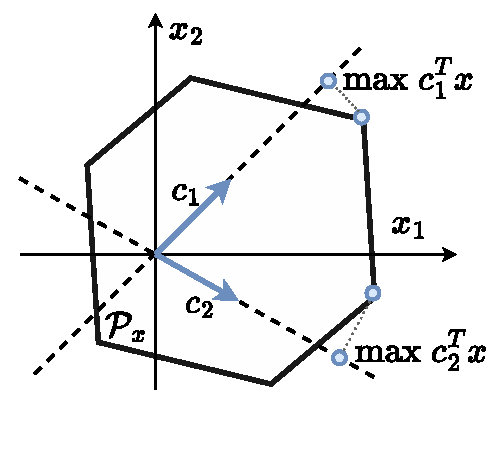
\includegraphics[width=\linewidth]{Papers/images/lp_explication.pdf}
    \caption{The figure demonstrates the \gls{lp} based vertex search by choosing two different vectors $\bm{c}$.}
    \label{fig:lp_explication}
\end{wrapfigure}
\subsection{Linear programming formulation}
\label{ch:lp_adapt}

From a geometrical point of view, solving a \gls{lp} problem boils down to finding a vertex of a polytope \cite{vajda_gass_1964}. 
\begin{equation}
\begin{aligned}
    \bm{x}_v = \text{arg}\max_{\bm{x}} \quad &  \bm{c}^T\bm{x} \\
     \textrm{s.t.} ~~&\bm{x} \in \mathcal{P}_x \\
\end{aligned}
\label{eq:lin_prog_generic}
\end{equation}
However, in order for the polytope $\mathcal{P}_x$ to be suitable for \gls{lp} optimisation in the $m$-dimensional output space, its implicit formulation $A\bm{x}=B\bm{y}$ needs to be expressed in explicit form.

In the general case, the input space is higher dimensional $n\geq m$ and the matrix $A$ is not square. As discussed in \Cref{par:equivalent_proj}, to find an explicit form of equation (\ref{eq:generic_polyt_view_revisit2}), the pseudo-inverse $A^+$ can be used as a solution only if $B\bm{y}+\bm{b}$ belongs to the image $\img{A}$ of $A$ \cite{klema_singular_1980}. Therefore, equation 
\begin{equation}
    A\bm{x} = B\bm{y} + \bm{b}
\end{equation} 
can be transformed to 
\begin{equation}
    \bm{x} = A^{+} (B \bm{y} + \bm{b}), \qquad \text{where} \quad B\bm{y} + \bm{b} \in \mathcal{I}m(A)
    \label{eq:eq_general_red}
\end{equation} 

Using the \gls{svd} \cite{klema_singular_1980} of the matrix $A^T$ produces $A^T = U\Sigma V^T$. The rotation matrix $V \in \mathbb{R}^{n\times n }$ is separated into  $V_1\in \mathbb{R}^{n\times m}$, a projector to the image $\img{A}$ of $A$, and $V_2\in \mathbb{R}^{n\times(n-m)}$, a projector to its null-space $\ker{A}$. As all the vectors belonging to the $\img{A}$ have zero projection to the null-space $\ker{A}$, an equality constraint can be devised for $B\bm{y}+\bm{b}$ to belong to the image $\img{A}$ of $A$. 
\begin{equation}
    V_2^TB\bm{y} +V_2^T\bm{b}  = \bm{0}
    \label{eq:nullspace_gen}
\end{equation}

Finally, combining equations (\ref{eq:nullspace_gen}), (\ref{eq:eq_general_red}), (\ref{eq:generic_poly_input_set_revisit2}) and (\ref{eq:generic_polyt_view_revisit2}), one can create a \glsxtrfull{lp} capable of reaching all vertices of the polytope $\mathcal{P}_x$
\begin{equation}
\begin{aligned}
    \max_{\bm{y}} \quad &  \bm{c}^TA^{+}B\bm{y} + A^{+}\bm{b}\\
     \textrm{s.t.} \quad &  V_2^TB\bm{y} = -V_2^T\bm{b} \\
          & ~~~  H_y \bm{y} \leq \bm{d}_y \\
\end{aligned}
\label{eq:lin_prog}
\end{equation}
by appropriately choosing the projection $\bm{c}$, as demonstrated on \Cref{fig:lp_explication}.



\subsection{Proposed ICHM algorithm overview}
\label{ch:method}

Given the polytope definition (\ref{eq:generic_polyt_view_revisit2}) and the \gls{lp} problem defined in (\ref{eq:lin_prog}), the proposed ICHM algorihtm provides a structured way to choose vectors $\bm{c}$ to find all the vertices ($\repr{V}$-representation) and facets ($\repr{H}$-representation) of the polytope $\mathcal{P}_x$. 
In order to do so, the method leverages the iterative Convex-Hull $\mathcal{C}$ calculation, where each newly found vertex extends $\mathcal{C}$. The normal vectors of the faces of the newly obtained $\mathcal{C}$ are used to decide for the new vectors $\bm{c}$ to use in the \gls{lp} (\ref{eq:lin_prog}). This iterative process is performed until some specified level of accuracy is reached. \Cref{fig:algo_example} visually demonstrates several iterations of the algorithm for the 2-dimensional polytope $\mathcal{P}_x$ example.

\subsubsection{Initial Convex-Hull}More precisely, the first step of the algorithm constructs an initial set of vertices $X_v$ and an initial Convex-Hull $\mathcal{C}$. In a $m$-dimensional space, the minimal number of points to create a volume is $m\!+\!1$.  There are various ways proposed in the literature to obtain the initial set of points in order to start the refinement process, such as starting by a random set of directions $\bm{c}$ proposed by \citet{lassez1992quantifier} in their original paper. Another approach, proposed by \citet{DelPrete2016Fast} proposes to uniformly sample the input space.

The approach proposed in this work exploits the base vectors $\bm{u}_i\in U$ obtained using the \gls{svd} of the matrix $(A^+B) = U\Sigma V^T$. This approach has two benefits. One one hand, the base vectors $\bm{u}_i$ are orthogonal vectors in the output space corresponding to the 
highest variability (amplification) directions, given by the singular values $\sigma_i$ of the matrix $A^+B$.
Therefore, the chances of not obtaining $m-1$ different vertices when projecting the polytope $\mathcal{P}_x$ in these directions is much lower than in random directions. And on the other hand, for any matrix $A$ and $B$, the matrix $U$ is relatively efficient to calculate.

Therefore, the proposed approach to find the initial set of vertices consists in solving two \glspl{lp} (\ref{eq:lin_prog}) for each one of the $m$ base vectors $\bm{u}_i$, one that minimises ($\bm{c} = -\bm{u}_i$) and one that maximises ($\bm{c} = \bm{u}_i$) the projection of the polytope $\mathcal{P}_x$. In the ideal case, this approach obtains $2m$ vertices of the polytope $\mathcal{P}_x$. Once the initial set of vertices $\bm{x}_v$ is found, the initial Convex-Hull $\mathcal{C}$ can be calculated. Its centroid position is given by $\bm{x}_c\!=\!\frac{1}{N}\!\sum\bm{x}_{v,i}$. 



\begin{figure}[!t]
    \centering
    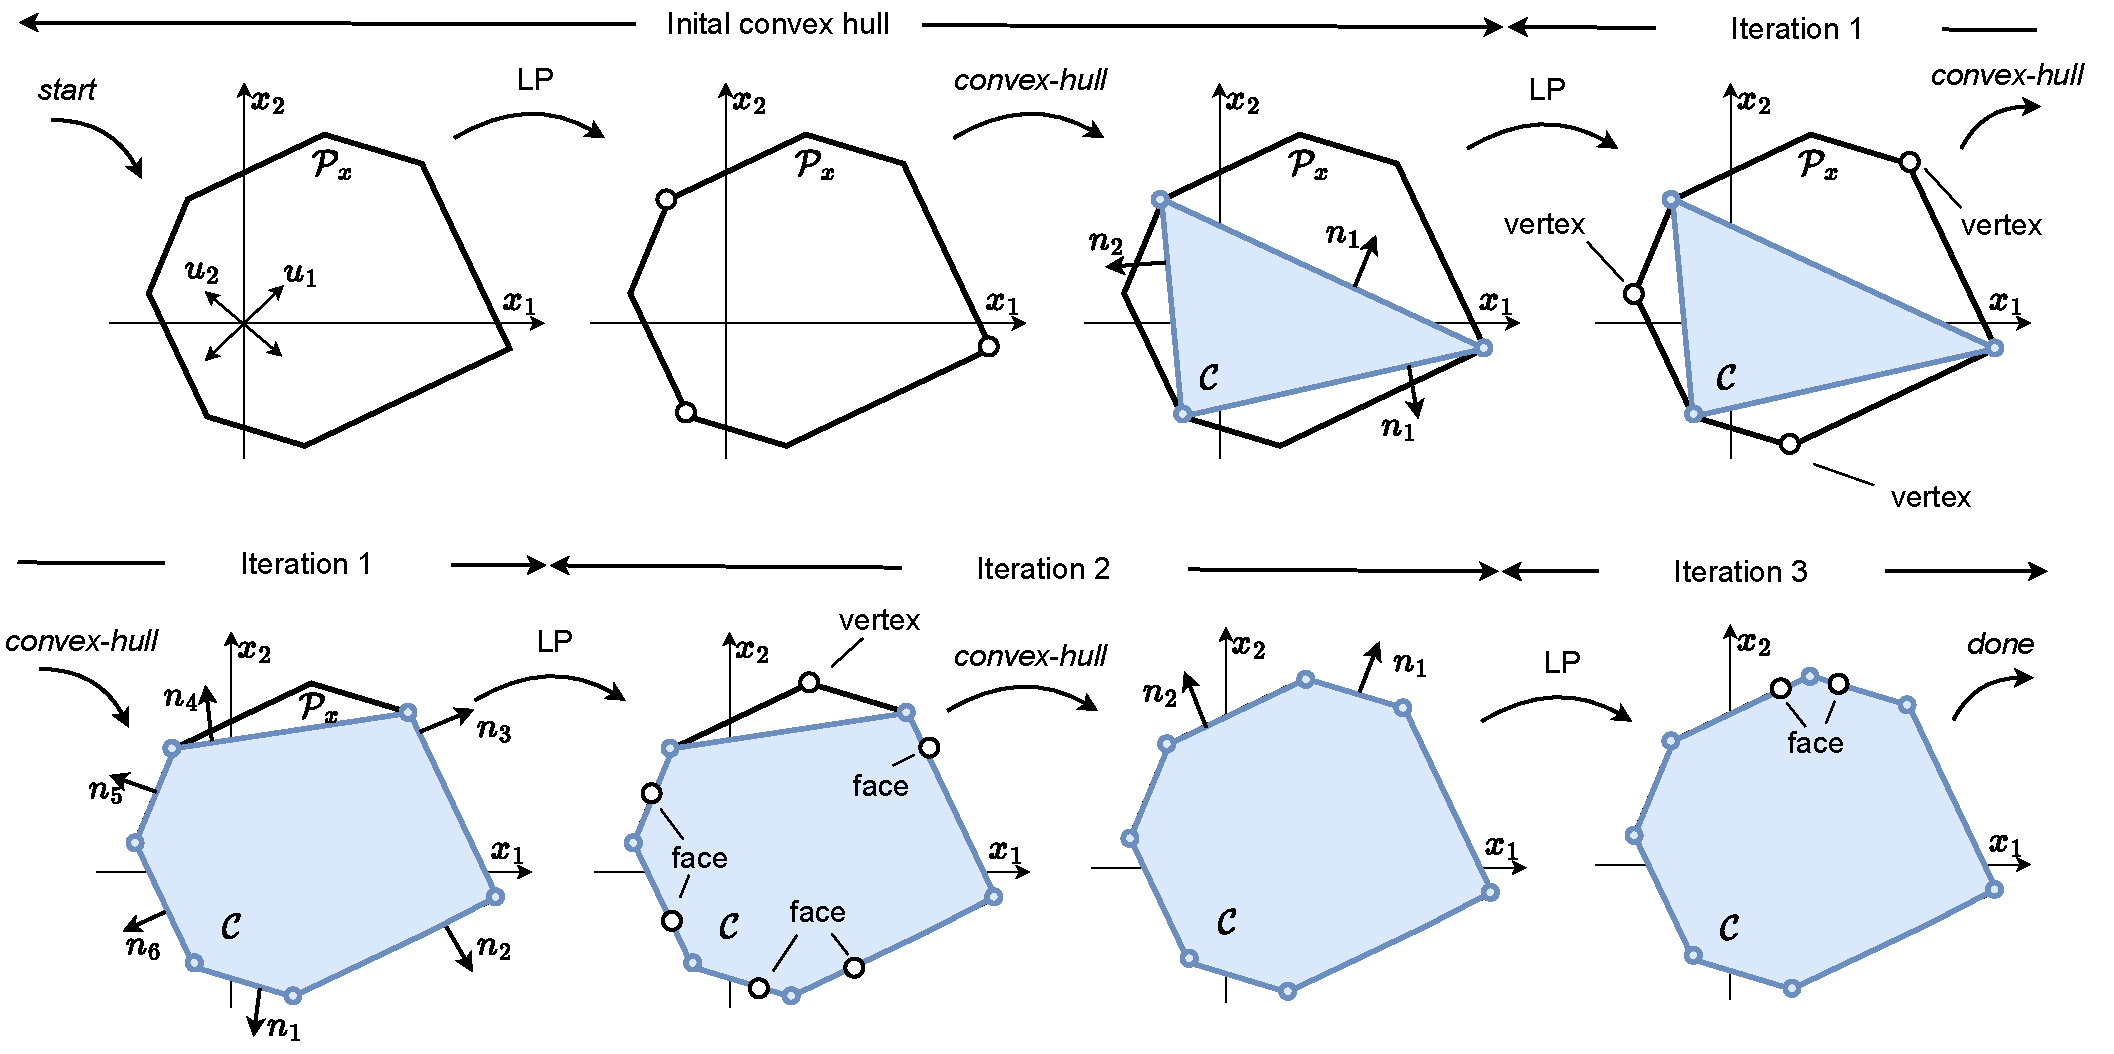
\includegraphics[width=\linewidth]{Papers/images/ichm_full.pdf}
    \vspace{-0.8cm}
    \caption{This figure shows the procedure of the successive approximation of the polytope $\mathcal{P}_x$ using the proposed ICHM algorithm. The approximation starts with the initial Convex-Hull $\mathcal{C}$ construction, using the vectors $\bm{u}_i\in U$. Then the approximation is refined by using the face normal vectors $\bm{n}_i$ of the Convex-Hull $\mathcal{C}$ with the \gls{lp} (\ref{eq:lin_prog}) to find new vertices which are then used to update the Convex-Hull $\mathcal{C}$. The check (\ref{eq:normal_coplanar_test}) is used to determine if the \gls{lp} results belong to the faces or they are new vertices of the polytope. The algorithm stops when no new vertices are found. }
    \label{fig:algo_example}
\end{figure}


\begin{wrapfigure}{r}{0.35\linewidth}
\vspace{-1.5cm}
    \centering
    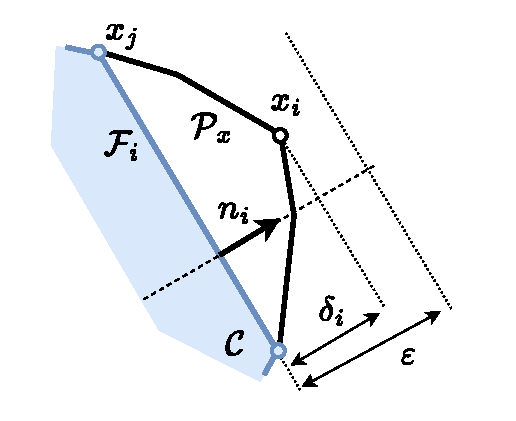
\includegraphics[trim=2.5cm 2cm 0 0,clip=true,width=\linewidth]{Papers/images/espilon_explicaiton.pdf}
    \caption{ The figure shows an example of the polytope face condition from equations (\ref{eq:normal_coplanar_test}) and (\ref{eq:normal_distance}). The face $\mathcal{F}_i$ of the Convex-Hull $\mathcal{C}$ is considered to be the face of $\mathcal{P}_x$, because $\delta_i\! < \!\varepsilon$. }
    \label{fig:expilon_explication}
\end{wrapfigure}
\subsubsection{Incremental refinement} The next step of the algorithm is to iterate over all the faces $\mathcal{F}_i$ of the Convex-Hull $\mathcal{C}$. For each new face $\mathcal{F}_i$, the normal $\bm{n}_i$ is found and used as a candidate $\bm{c}_i$ in the direction pointing out of polytope $\mathcal{P}_x$.
%all the vertices $\bm{x}_{\mathcal{F}j}\! =\! %\bm{x}_v\!\in\!\mathcal{F}_i$. Then the $\bm{c}_i$ is defined %as normal $\bm{n}_i$ in the direction pointing out of the polytope 5$\mathcal{P}_x$.
The normal vector direction is verified by projecting the vector going from the centroid $\bm{x}_c$ to any vertex $\bm{x}_{j}$ of face $\mathcal{F}_i$, onto the normal $\bm{n}_i$ and verifying if the scalar product is positive or negative.\\
\begin{equation}
    \bm{c}_i = \begin{cases}
  \bm{n}_i, & \text{if } \bm{n}_i^T(\bm{x}_{j} - \bm{x}_c) \geq 0, \\
  -\bm{n}_i, & \text{otherwise}.
\end{cases} 
\label{eq:normal_condition}
\end{equation}
Solving equation (\ref{eq:lin_prog}) with $\bm{c}_i$, the obtained $\bm{x}_i$ can be either a vertex of the polytope $\mathcal{P}_x$ or be coplanar with face $\mathcal{F}_i$. To determine if  $\bm{x}_i$ is coplanar with the face, a simple check can be devised, which verifies if the orthogonal (normal) distance from $\bm{x}_i$ to any vertex $\bm{x}_{j}$ of face $\mathcal{F}_i$
\begin{equation}
    \delta_i = \bm{n}_i^T(\bm{x}_{j} - \bm{x}_i)
\label{eq:normal_distance}
\end{equation}
is within a certain user defined accuracy $\varepsilon$
\begin{equation}
    \bm{x}_i = \begin{cases}
   \text{vertex}, & \text{if }  |\delta_i| \geq \varepsilon, \\
    \text{on the face}, & \text{otherwise}.
\end{cases} 
\label{eq:normal_coplanar_test}
\end{equation}
\Cref{fig:expilon_explication} provides a graphical interpretation of this check and of the values $\delta_i$ and $\varepsilon$.

If $\bm{x}_i$ belongs to face $\mathcal{F}_i$ of the Convex-Hull $\mathcal{C}$ then  $\mathcal{F}_i$ is considered to be a face of the polytope $\mathcal{P}_x$. In that case the algorithm updates the $\repr{H}$-representation of $\mathcal{P}_x$ 
\begin{equation}
    H \leftarrow \begin{bmatrix} H \\ \bm{n}_i^T\end{bmatrix}, \quad \bm{d} \leftarrow \begin{bmatrix}  \bm{d} \\ \bm{n}^T_i \bm{x}_{j} \end{bmatrix}
\label{eq:h_rep}
\end{equation}
where $\bm{n}_i$ is the face normal vector and $\bm{n}_i^T \bm{x}_{j}$ is the orthogonal distance from the origin to the face $\mathcal{F}_i$. On the other hand, if $\bm{x}_i$ is a vertex of the polytope it is appended to the $\repr{V}$-representation list $X_v \leftarrow [X_v, ~\bm{x}_i]$.

\subsubsection{Stopping condition} 
Once all the faces of the Convex-Hull $\mathcal{C}$ are evaluated, the Convex-Hull is updated using the new vertex list $X_v$.

One of the algorithm stopping conditions proposed by \citet{Bretl2008}, is to construct the inner and outer approximation of the polytope $\mathcal{P}_x$ at the same time and stop approximating when the ratio $r=\vol{\mathcal{P}_{inner}}/\vol{\mathcal{P}_{outer}}$ between their volumes reaches a certain threshold $r\leq1$.  

However, volume ratio condition is sometimes hard to interpret, as its representation of the approximation error does not have the same units as the physical quantity being represented by the polytope $\mathcal{P}_x$. Therefore, the ICHM algorithm exploits a different stopping condition setting the threshold on the maximal distance $\delta_i$. The algorithm stops iterating if the vertex list $X_v$ has no new elements or, in other words, if the maximal distance $\delta_i$ for all the faces $\mathcal{F}_i$ is lower than the user defined accuracy $\varepsilon$  
\begin{equation}
    \max\{|\delta_{i}|\} \leq \varepsilon
\end{equation}
In this stopping condition, the maximal distance $\delta_i$ corresponds to the maximal error committed by the approximation, expressed with the same units as the units of the physical quantity being represented by the polytope. Provided that the output space has the same units in all the axis. Preserving the same units improves the interpretation of the approximation error and enables the user to intuitively decide on the acceptable approximation error $\varepsilon$ for the application in question. 

Finally, if the user sets the approximation error $\varepsilon\!=\!0$, the ICHM algorithm finds the exact solution, all the vertices and the faces of the polytope $\mathcal{P}_x$.

\subsection{Performance analysis}
\label{ch:chm_performance}

To evaluate the efficiency of the ICHM algorithm, the challenging polytope formulation, corresponding to the generic formulation (\ref{eq:generic_polyt_view_revisit2}), with a high-dimensional input space and a low-dimensional output space ($n\gg m$) is tested. Additionally, the algorithm performance is compared against two state-of-the-art approaches: an approximation approach based on the \gls{rsm} algorithm introduced by \citet{carmichael_towards_2011} and an exact evaluation approach based on the combination of two efficient algorithms \gls{hpsm} \cite{hyper_psm} and \gls{pim} \cite{bremner_fukuda_marzetta_1998}.

\subsubsection{Human wrench capacity polytope}
The polytope in question is the human's wrench capacity polytope, previously discussed in \Cref{ch:force_poly_human}. The polytope $\mathcal{P}_f$ characterising the achievable wrenches $\bm{f}$, the human can generate given its musculoskeletal model, can be expressed as 
\begin{equation}
    \mathcal{P}_f(\bm{q},\dot{\bm{q}},\ddot{\bm{q}}) = \left\{ \bm{f} \in \mathbb{R}^m ~|~ \bm{F}\in\left[\bm{F}_{min}, \bm{F}_{max} \right], ~~ \!J^T(\bm{q})\bm{f} =\! N(\bm{q})\bm{F} -\bm{\tau}_b(\bm{q},\dot{\bm{q}},\ddot{\bm{q}}) \right\}
    \label{eq:human_force_poly_revisit2}
\end{equation}
where $\bm{f}\in\mathbb{R}^m$ is the \gls{cs} wrench, $\bm{F}\in\mathbb{R}^n$ is the vector of muscular forces, while $J(\bm{q})$ and $N(\bm{q})$ are configuration $\bm{q}$ dependant Jacobian and moment arm matrix. Additionally, the bias vector $\bm{\tau}_b$ corresponds to the joint torques corresponding to the effects of the gravity and the movement. 

% \begin{landscape}
\begin{figure}[!t]
    \centering
    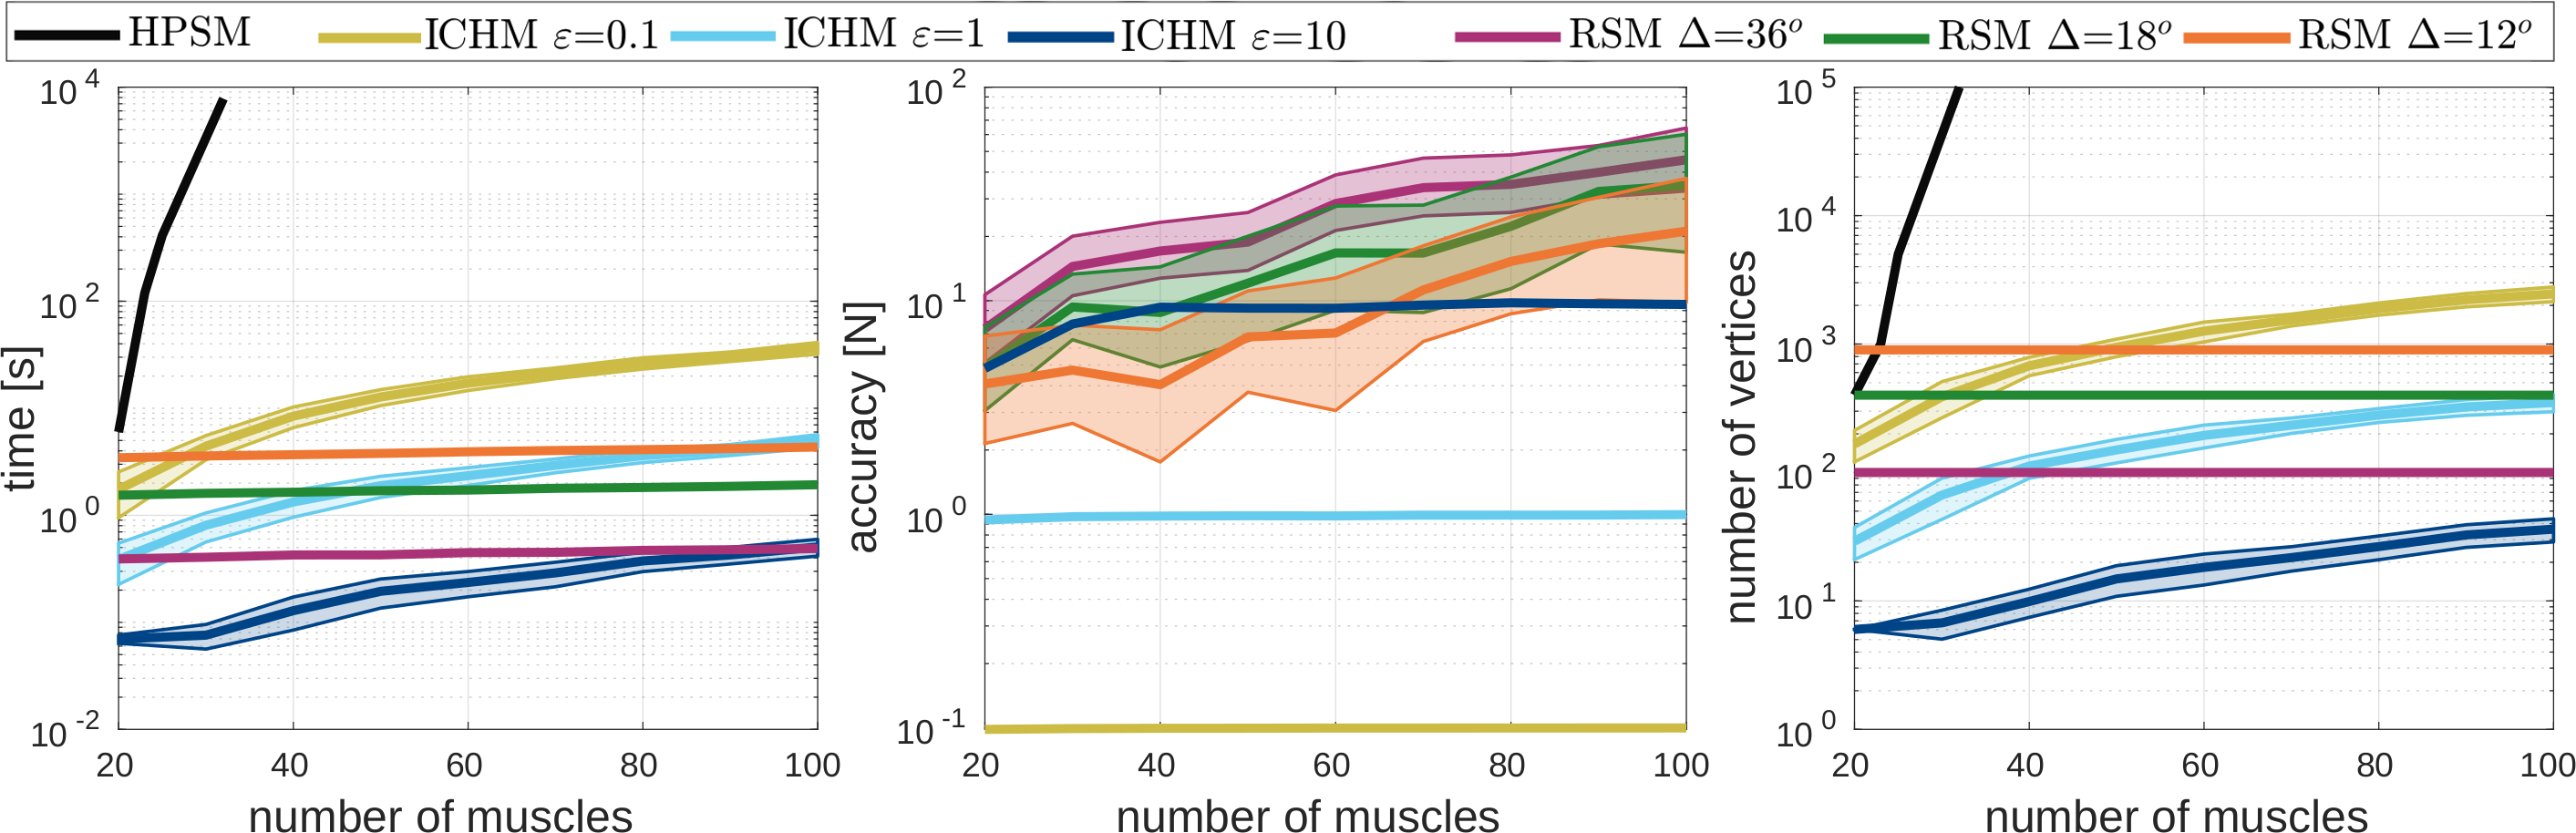
\includegraphics[width=\linewidth]{Papers/images/one_auto_new5_these.png}
    \caption{{Figure presenting the performance analysis results in the logarithmic scale for three different algorithms: \gls{hpsm}, \gls{rsm} and proposed ICHM with respect to different number of muscles. The left figure shows the evolution of the execution time. The middle figure shows the evolution of the underestimation error, the maximal distance in between the polytope $\mathcal{P}_x$ and the acquired polytope, calculated as max$\{|\delta_{i}|\}$. The right figure shows the evolution of the number of vertices found. All the plots show the averaged results, with variances, over 100 runs, where each run corresponds to one randomly generated model.}}
    \label{fig:performance_results}
\end{figure}
% \end{landscape}
This polytope formulation is challenging due to the high dimensional input space (large number of muscles), making the geometry of the polytope $\mathcal{P}_f$ relatively complex, having large number of faces and vertices. In such cases, standard exact methods for polytope transformation have long execution times, preventing this polytope representation to be used in interactive (online) applications. To reduce the computation times of the wrench polytope $\mathcal{P}_f$ evaluation, \citet{carmichael_towards_2011} have proposed an algorithm based on the \gls{rsm}, described in \Cref{ch:approximation_algos}. Although the algorithm enables real-time approximation of the polytope $\mathcal{P}_f$, the obtained approximation is coarse and without any bounds on the approximation accuracy. 


\subsubsection{Experiment and results}
Therefore, to evaluate the performance of the proposed ICHM algorithm, a comparative experiment is
performed, where the ICHM algorithm's performance is compared against the \gls{rsm} method proposed by \citet{carmichael_towards_2011} as well as against the two step exact approach based on the \gls{hpsm} \cite{hyper_psm} and \gls{pim} \cite{bremner_fukuda_marzetta_1998}. The experiment consists in finding the $\repr{V}$-representation of the \gls{cs} force $m=3$ polytope $\mathcal{P}_f$ for a randomised mock-up musculoskeletal model with $k\!=\!7$ degrees of freedom and a number of muscles ranging from $n$ = $20$ to $100$. 

The \gls{rsm} algorithm \cite{carmichael2011Towards} requires uniform sampling of the ray directions in the 3D space. In this experiment the sampling is performed based on a two Euler angles parametrisation. {For this method, three linearly increasing levels of granularity are tested for each Euler angle: $\Delta\!=\!36^o$, $18^o$ and $12^o$;  making for $n_r\!=\!10,20$ and $30$ rays per angle. Overall number of ray directions in 3D space ($N_r\!=\!n_r^2$) is then $100$, $400$ and $900$. For the proposed ICHM algorithm, three exponentially increasing levels of accuracy are tested $\varepsilon\!=\!0.1$, $1$ and $10$ N.} All the algorithms are implemented in Matlab and run on a 1.90GHz Intel i7-8650U processor. The source code of the experiment is publicly available on GitLab\footnote{Gitlab: \url{https://gitlab.inria.fr/auctus-team/people/antunskuric/papers/human_wrench_capacity}}.

Results of the experiments, averaged over 100 algorithm runs, are shown on \Cref{fig:performance_results}. The results confirm that the exact approach using the \gls{hpsm} method has an execution time exponentially related to the number of muscles. Even for only 30 muscles it already takes more than 4.5 h to calculate, therefore this method is not tested on more than 30 muscles, where it finds over $10^4$ vertices.  

\begin{figure}[!t]
    \centering
    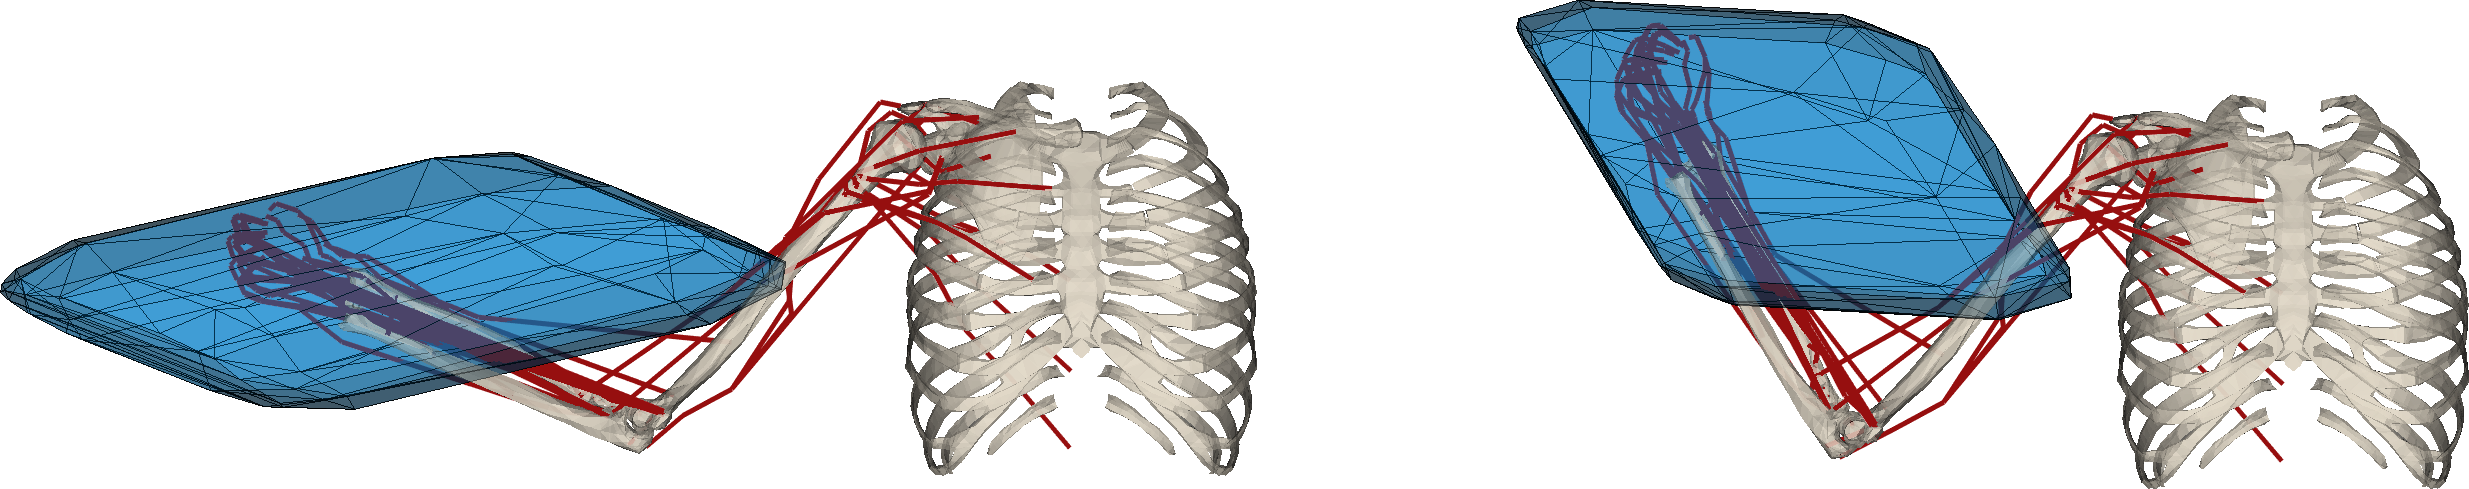
\includegraphics[width=\linewidth]{Papers/images/force.png}
    \caption{\gls{cs} force polytope of a musculoskeletal model of human upper limb  \cite{saul2015benchmarking} with 7DOF and 50 muscles, evaluated for two different configurations using the proposed ICHM algorithm. The visualisation is performed using \codet{bioviz} \cite{Michaud2021} and polytopes are scaled with a ratio 1m : 1000N}
    \label{fig:images_bimanual}
\end{figure}
The \gls{rsm} algorithm shows nearly constant time of execution for the full range of tested muscles and the constant number of vertices found, which is expected. The results show however, that for low muscle numbers $d\!<$25, when using a fine granularity $\Delta$=$12^o$ the \gls{rsm} algorithm finds more vertices than the exact solution found by the \gls{hpsm}. Furthermore, the middle plot of \Cref{fig:performance_results} shows that the \gls{rsm} estimation error increases considerably with the number of muscles $d$, followed by a very
high variance. These results confirm that, as the polytope shape is not spherical, by uniformly covering the space of ray directions, \gls{rsm} based algorithms will necessarily estimate certain areas of the polytope better than the others.

The graphs show that the proposed ICHM method's execution time depends near-linearly of the number of muscles considered $d$ and the estimation error bound parameter $\varepsilon$. The accuracy graph, shown in the middle plot, shows that the proposed ICHM algorithm is capable of limiting the estimation error of the polytope evaluation under desired value $\varepsilon$ regardless of the number of muscles. Furthermore, considering the vertex number found by the algorithms, it can be seen that the number of vertices has a nearly-linear relationship with the number of muscles $d$ and the variable $\varepsilon$. 

The demonstrated efficiency of the ICHM algorithm opens many doors for its applications in real-time systems, providing the user with an easy to understand trade-off between speed and accuracy. 
\Cref{fig:images_bimanual} shows the visualisation of the \gls{cs} force ($m=3$) polytope of a human musculoskeletal model with 50 muscles and 7DOFs, calculated using the ICHM algorithm.


\newpage
\subsection{Algorithm implementation}
\qrimg{qrcodes/pycapacity.png}{https://auctus-team.github.io/pycapacity/}{\codet{pycapacity}}
The pseudo-code of the ICHM algorithm is given in \Cref{alg:algo_2}, while an efficient open-source Python implementation is publicly available within the package \codet{pycapacity}\footnote{\href{https://auctus-team.github.io/pycapacity/}{https://auctus-team.github.io/pycapacity/}}, which is described more in detail in \Cref{ch:software}.

Finally, \Cref{ch:human_robot_carrying} brings the application of the proposed algorithm for the real-time robot control in the human-robot collaboration scenario, where the algorithm is exploited in order to calculate the human's wrench capacity polytope online. 


\begin{algorithm}[!h]
\caption{Proposed ICHM algorithm pseudo-code}
\begin{algorithmic}
\REQUIRE $A$,$B$, $\bm{y}_{min}$, $\bm{y}_{max}$, $\bm{b}$, $\varepsilon$
\STATE $U, \Sigma, V^T \leftarrow svd(A^+)$ 

\STATE init $\repr{H}$-rep: $H,\bm{d} \leftarrow [\,]$ and $\repr{V}$-rep: $\bm{x}_v,\bm{y}_v\leftarrow [\,]$
\STATE \textbf{for all}   {$\bm{u}_i$ in $U$} \textbf{do}

\hspace{0.3cm} $\bm{y}_{i}\leftarrow$ \gls{lp} (Eq. \ref{eq:lin_prog}) with $\bm{c}\! =\! \bm{u}_i$ and $\bm{c}\! =\! -\bm{u}_i$

\hspace{0.3cm} $\bm{x}_{v} \leftarrow [\bm{x}_{v}, ~ A^+B\bm{y}_i + A^+\bm{b}]$

\REPEAT

\STATE calculate the Convex-Hull $\mathcal{C}$ of $\bm{x}_{v}$
\STATE calculate the centroid $\bm{x}_{c} = \frac{1}{N}\sum_i\bm{x}_{v,i}$

\STATE \textbf{for all}   {new face $\mathcal{F}_i$ in $\mathcal{C}$} \textbf{do}
%\FORALL{ new face $\mathcal{F}_i$ in $\mathcal{C}$ } 

\hspace{0.25cm} find normal $\bm{n}_i$ and one vertex $\bm{x}_{j}$ of $\mathcal{F}_i$

\hspace{0.25cm} $\bm{y}_{i}\leftarrow$ \gls{lp} ( Eq. \ref{eq:lin_prog} ) with  $\bm{c}\! =\! \bm{n}_i$ ( Eq. \ref{eq:normal_condition} )

\hspace{0.25cm} $\bm{x}_{i} = A^+B\bm{y}_i+A^+\bm{b}$ 

\hspace{0.25cm}  calculate $\delta_i$ (Eq.\ref{eq:normal_distance})

\hspace{0.25cm}  \textbf{if}   $ |\delta_i| \leq \varepsilon$ \textbf{then} 

\hspace{0.6cm}  new face: update $\repr{H}$-rep  ( Eq. \ref{eq:h_rep} )

\hspace{0.25cm}  \textbf{else}

\hspace{0.6cm} new vertex: update $\repr{V}$-rep: $\bm{x}_{v} \!\leftarrow\! [\bm{x}_{v},~ \bm{x}_i ]$,  $\bm{y}_{v} \!\leftarrow\! [\bm{y}_{v},~ \bm{y}_i ]$ 

%\ENDFOR
\UNTIL{{ $\max\{|\delta_{i}|\}\leq \varepsilon$}}
\RETURN  $\repr{V}$-rep: $\bm{x}_v$, $\bm{y}_v$ and  $\repr{H}$-rep: $H$, $\bm{d}$ 
\end{algorithmic}
\label{alg:algo_2}
\end{algorithm}

\section{Conclusion}

This chapter aims to provide a set of tools for efficient transforming of polytopes representing the physical abilities of humans and robots into more standardised forms suitable for practical applications. The focus is put on the two widely used polytope representations: vertex or $\repr{V}$ and half-plane or $\repr{H}$-representations. These representations offer various advantages, including compatibility with visualisation tools, in a for triangulated meshes, and optimisation-based applications like robot control and trajectory planning. Additionally, they enable efficient operations like Minkowski sums and intersections over multiple polytopes.

While the literature presents numerous algorithms for transforming polytope formulations into their $\repr{H}$ or $\repr{V}$-representation, these algorithms are often tailored to specific sets of polytope formulations. \Cref{ch:phisical_ability_metrics} proposes a generic view on different common polytope representation of humans' and robots' physical abilities and proposed a unifying polytope formulation describing all the proposed metrics, introduced in \Cref{ch:collab_metrics_overview}. However, this unified formulation is not directly suitable for the standard polytope transformation algorithms. Hence, \Cref{ch:generic_view} proposes a structured view on different polytope formulation families derived from the proposed generic unified formulation namely intersection and projection formulation, as well as some special cases.

\Cref{ch:polytope_algorithms} further provides an overview of applicable techniques for transforming these families into their $\repr{V}$ or $\repr{H}$-representation. The chapter briefly introduces the standard generic methods for mutual transformation between $\repr{V}$ and $\repr{H}$-representation, followed by the polytope formulation specific methods that are capable of better exploiting the geometry of the formulation families. Finally, several polytope approximation methods are discussed as a means of improving the efficiency of polytope transformation for high-dimensional problems. 
The aim of this overview is to provide a brief introduction into the applicable state-of-the-art methods when it comes to transforming different polytope formulations as well as to discuss their limitations and computational efficiency.

The final two sections of this chapter introduce two contributions of this thesis in the domain of polytope transformations. The \Cref{sec:algorithm_vea} introduces an efficient vertex enumeration algorithm for the intersection polytope formulation with the interval input set. This algorithm is based on the work by \citet{sasaki2011vertex}, exploiting the geometry of the hyperrectangle input set in order to improve its computational complexity of its exhaustive search and reduce the execution time. The algorithm is particularly well suited for low dimensional polytope evaluation, that are common when it comes to polytope characterisations of physical abilities of robotic manipulators. The performance of the proposed algorithm is compared to the state-of-the-art methods on finding the $\repr{V}$-representation of the force capacity polytope for redundant robotic manipulators, introduced in \Cref{ch:poly_force}. The results show that the algorithm has significantly lower computational complexity and hence shorter execution time, in the order of magnitude of several milliseconds for standard robotic manipulators, implemented in Pyhton. Such short execution time opens doors for using these polytopes in real time applications, such as robot control. This algorithm has been published in the context of the scientific paper \citet{skuric2021robot}.

\Cref{ch:algorihtm_ichm} brings a new polytope approximation algorithm based on the \gls{chm} by \citet{lassez1992quantifier}. The algorithm is developed for the generic polytope formulation directly and can therefore be used with all the common polytope formulation introduced in previous chapter. This algorithm performs an iterative approximation of the final polytope by using sequences of \glspl{lp} to find new vertices of the polytope and Convex-Hull to group the to faces. The algorithm improves the approximation accuracy in each iteration and continues iterating when desired user defined approximation accuracy is reached. The execution time of the algorithm depends directly of the complexity of the polytope being transformed (number of faces and verteices), therefore by appropriately setting the desired accuracy, the algorithm is capable of simplifying the final geometry of the polytope and lowering the execution time. This is particularly useful when it comes to the high-dimensional problems, where the input space dimension is much higher than the output space $n\!\gg \!m$, where the standard exact methods have intractable execution times, as they are based on different forms of the exhaustive search. Such high-dimensional problems are very common when it comes to characterising physical abilities of humans based on their musculoskeletal models, as they often have large number of muscles $n$, while their capacities are characterised in the \gls{cs} $m=3$. The performance of the proposed method is therefore tested on the challenging polytope formulation of the human's wrench capacity polytope, described in \Cref{ch:force_poly_human}. The results of the proposed methods in comparison to the state-of-the-art methods show that it has significantly shorter computation time while at the same time guaranteeing the user defined approximation accuracy. Furthermore, the results show that the proposed algorithm, in the case of human's wrench capacity polytope, has execution time under half of a seconds for musculoskeletal models up to 100 muscles, opening many doors for using this polytope formulation in the real time applications. The ICHM algorithm has been published in the context of the scientific paper \citet{Skuric2022human} and later refined within \citet{skuric2023dynamics}.

Following chapter leverages the proposed algorithms and formulations to propose several use-cases of the polytope based physical ability characterisations in the context of the real-time robot control in different human robot physical collaboration scenarios. 
\Cref{ch:physical_interaction} proposes uses the real-time polytope evaluation for creating more adapted robot control strategies in the context of the physical human-robot interaction. 
\Cref{ch:informaiton_polytopes} explores the possibilities of using polytopes for the real-time visual feedback to the operators. Moreover, \Cref{ch:topca} proposes a new \gls{cs} trajectory planning strategy exploiting the polytope algebra. Finally, \Cref{ch:software} presents the publicly available open-source software package implementing several algorithms introduced in this section and enabling an efficient, real-time compatible, evaluation of polytope based physical abilities for humans and robots.
